\subsection{Step Response}
After completing a simulation of the system's step response, the plot shown
in Figure~\ref{f:stepSim} was produced by PSpice.
%
\begin{figure}[H]
	\centering
	\begin{tikzpicture}[gnuplot]
%% generated with GNUPLOT 4.4p2 (Lua 5.1.4; terminal rev. 97, script rev. 96a)
%% Sun 27 Nov 2011 03:28:34 PM EST
\gpsolidlines
\gpcolor{gp lt color axes}
\gpsetlinetype{gp lt axes}
\gpsetlinewidth{1.00}
\draw[gp path] (1.136,0.985)--(7.854,0.985);
\gpcolor{gp lt color border}
\gpsetlinetype{gp lt border}
\draw[gp path] (1.136,0.985)--(1.316,0.985);
\node[gp node right] at (0.952,0.985) {-1};
\gpcolor{gp lt color axes}
\gpsetlinetype{gp lt axes}
\draw[gp path] (1.136,1.529)--(7.854,1.529);
\gpcolor{gp lt color border}
\gpsetlinetype{gp lt border}
\draw[gp path] (1.136,1.529)--(1.316,1.529);
\node[gp node right] at (0.952,1.529) { 0};
\gpcolor{gp lt color axes}
\gpsetlinetype{gp lt axes}
\draw[gp path] (1.136,2.072)--(7.854,2.072);
\gpcolor{gp lt color border}
\gpsetlinetype{gp lt border}
\draw[gp path] (1.136,2.072)--(1.316,2.072);
\node[gp node right] at (0.952,2.072) { 1};
\gpcolor{gp lt color axes}
\gpsetlinetype{gp lt axes}
\draw[gp path] (1.136,2.616)--(7.854,2.616);
\gpcolor{gp lt color border}
\gpsetlinetype{gp lt border}
\draw[gp path] (1.136,2.616)--(1.316,2.616);
\node[gp node right] at (0.952,2.616) { 2};
\gpcolor{gp lt color axes}
\gpsetlinetype{gp lt axes}
\draw[gp path] (1.136,3.159)--(7.854,3.159);
\gpcolor{gp lt color border}
\gpsetlinetype{gp lt border}
\draw[gp path] (1.136,3.159)--(1.316,3.159);
\node[gp node right] at (0.952,3.159) { 3};
\gpcolor{gp lt color axes}
\gpsetlinetype{gp lt axes}
\draw[gp path] (1.136,3.703)--(7.854,3.703);
\gpcolor{gp lt color border}
\gpsetlinetype{gp lt border}
\draw[gp path] (1.136,3.703)--(1.316,3.703);
\node[gp node right] at (0.952,3.703) { 4};
\gpcolor{gp lt color axes}
\gpsetlinetype{gp lt axes}
\draw[gp path] (1.136,4.246)--(7.854,4.246);
\gpcolor{gp lt color border}
\gpsetlinetype{gp lt border}
\draw[gp path] (1.136,4.246)--(1.316,4.246);
\node[gp node right] at (0.952,4.246) { 5};
\gpcolor{gp lt color axes}
\gpsetlinetype{gp lt axes}
\draw[gp path] (1.136,4.790)--(7.854,4.790);
\gpcolor{gp lt color border}
\gpsetlinetype{gp lt border}
\draw[gp path] (1.136,4.790)--(1.316,4.790);
\node[gp node right] at (0.952,4.790) { 6};
\gpcolor{gp lt color axes}
\gpsetlinetype{gp lt axes}
\draw[gp path] (1.136,0.985)--(1.136,4.790);
\gpcolor{gp lt color border}
\gpsetlinetype{gp lt border}
\draw[gp path] (1.136,0.985)--(1.136,1.165);
\node[gp node center] at (1.136,0.677) { 0};
\gpcolor{gp lt color axes}
\gpsetlinetype{gp lt axes}
\draw[gp path] (2.480,0.985)--(2.480,4.790);
\gpcolor{gp lt color border}
\gpsetlinetype{gp lt border}
\draw[gp path] (2.480,0.985)--(2.480,1.165);
\node[gp node center] at (2.480,0.677) { 2};
\gpcolor{gp lt color axes}
\gpsetlinetype{gp lt axes}
\draw[gp path] (3.823,0.985)--(3.823,4.790);
\gpcolor{gp lt color border}
\gpsetlinetype{gp lt border}
\draw[gp path] (3.823,0.985)--(3.823,1.165);
\node[gp node center] at (3.823,0.677) { 4};
\gpcolor{gp lt color axes}
\gpsetlinetype{gp lt axes}
\draw[gp path] (5.167,0.985)--(5.167,4.790);
\gpcolor{gp lt color border}
\gpsetlinetype{gp lt border}
\draw[gp path] (5.167,0.985)--(5.167,1.165);
\node[gp node center] at (5.167,0.677) { 6};
\gpcolor{gp lt color axes}
\gpsetlinetype{gp lt axes}
\draw[gp path] (6.510,0.985)--(6.510,4.790);
\gpcolor{gp lt color border}
\gpsetlinetype{gp lt border}
\draw[gp path] (6.510,0.985)--(6.510,1.165);
\node[gp node center] at (6.510,0.677) { 8};
\gpcolor{gp lt color axes}
\gpsetlinetype{gp lt axes}
\draw[gp path] (7.854,0.985)--(7.854,4.790);
\gpcolor{gp lt color border}
\gpsetlinetype{gp lt border}
\draw[gp path] (7.854,0.985)--(7.854,1.165);
\node[gp node center] at (7.854,0.677) { 10};
\draw[gp path] (1.136,4.790)--(1.136,0.985)--(7.854,0.985)--(7.854,4.790)--cycle;
\node[gp node center,rotate=-270] at (0.246,2.887) {Voltage (\si{\volt})};
\node[gp node center] at (4.495,0.215) {Time (\si{\milli\second})};
\node[gp node center] at (4.495,5.252) {Simulated Impulse Response of Third-order Low Pass Filter};
\draw[gp path] (8.222,2.579)--(8.222,3.195)--(10.610,3.195)--(10.610,2.579)--cycle;
\draw[gp path] (8.222,3.195)--(10.610,3.195);
\node[gp node right] at (9.326,3.041) {Input};
\gpcolor{gp lt color 0}
\gpsetlinetype{gp lt plot 0}
\gpsetlinewidth{2.00}
\draw[gp path] (9.510,3.041)--(10.426,3.041);
\draw[gp path] (1.136,1.529)--(1.136,1.583)--(1.136,1.637)--(1.136,1.746)--(1.136,1.963)%
  --(1.136,2.398)--(1.136,3.268)--(1.136,4.246)--(1.137,4.246)--(1.138,4.246)--(1.139,4.246)%
  --(1.141,4.246)--(1.144,4.246)--(1.148,4.246)--(1.155,4.246)--(1.167,4.246)--(1.186,4.246)%
  --(1.220,4.246)--(1.273,4.246)--(1.333,4.246)--(1.404,4.246)--(1.491,4.246)--(1.575,4.246)%
  --(1.669,4.246)--(1.778,4.246)--(1.838,4.246)--(1.914,4.246)--(1.989,4.246)--(2.041,4.246)%
  --(2.043,4.246)--(2.046,4.246)--(2.052,4.246)--(2.056,4.192)--(2.056,3.926)--(2.056,3.393)%
  --(2.056,2.328)--(2.056,1.529)--(2.057,1.529)--(2.058,1.529)--(2.060,1.529)--(2.063,1.529)%
  --(2.071,1.529)--(2.084,1.529)--(2.109,1.529)--(2.146,1.529)--(2.192,1.529)--(2.237,1.529)%
  --(2.302,1.529)--(2.383,1.529)--(2.468,1.529)--(2.566,1.529)--(2.628,1.529)--(2.709,1.529)%
  --(2.758,1.529)--(2.816,1.529)--(2.868,1.529)--(2.929,1.529)--(2.983,1.583)--(2.983,1.849)%
  --(2.983,2.382)--(2.983,3.447)--(2.983,4.246)--(2.984,4.246)--(2.985,4.246)--(2.987,4.246)%
  --(2.991,4.246)--(2.998,4.246)--(3.012,4.246)--(3.034,4.246)--(3.069,4.246)--(3.122,4.246)%
  --(3.182,4.246)--(3.253,4.246)--(3.342,4.246)--(3.426,4.246)--(3.520,4.246)--(3.629,4.246)%
  --(3.687,4.246)--(3.762,4.246)--(3.837,4.246)--(3.890,4.246)--(3.891,4.246)--(3.894,4.246)%
  --(3.900,4.246)--(3.904,4.192)--(3.904,3.926)--(3.904,3.393)--(3.904,2.328)--(3.904,1.529)%
  --(3.905,1.529)--(3.906,1.529)--(3.907,1.529)--(3.911,1.529)--(3.918,1.529)--(3.931,1.529)%
  --(3.957,1.529)--(3.994,1.529)--(4.039,1.529)--(4.085,1.529)--(4.149,1.529)--(4.231,1.529)%
  --(4.315,1.529)--(4.414,1.529)--(4.475,1.529)--(4.556,1.529)--(4.605,1.529)--(4.663,1.529)%
  --(4.716,1.529)--(4.777,1.529)--(4.831,1.583)--(4.831,1.849)--(4.831,2.382)--(4.831,3.447)%
  --(4.831,4.246)--(4.832,4.246)--(4.833,4.246)--(4.834,4.246)--(4.838,4.246)--(4.845,4.246)%
  --(4.859,4.246)--(4.881,4.246)--(4.916,4.246)--(4.969,4.246)--(5.029,4.246)--(5.101,4.246)%
  --(5.189,4.246)--(5.274,4.246)--(5.367,4.246)--(5.476,4.246)--(5.535,4.246)--(5.609,4.246)%
  --(5.685,4.246)--(5.737,4.246)--(5.739,4.246)--(5.742,4.246)--(5.747,4.246)--(5.751,4.192)%
  --(5.751,3.926)--(5.751,3.393)--(5.751,2.328)--(5.751,1.529)--(5.752,1.529)--(5.753,1.529)%
  --(5.755,1.529)--(5.758,1.529)--(5.765,1.529)--(5.779,1.529)--(5.804,1.529)--(5.841,1.529)%
  --(5.886,1.529)--(5.932,1.529)--(5.997,1.529)--(6.078,1.529)--(6.163,1.529)--(6.261,1.529)%
  --(6.323,1.529)--(6.403,1.529)--(6.452,1.529)--(6.511,1.529)--(6.563,1.529)--(6.624,1.529)%
  --(6.678,1.583)--(6.678,1.849)--(6.678,2.382)--(6.678,3.447)--(6.678,4.246)--(6.679,4.246)%
  --(6.680,4.246)--(6.682,4.246)--(6.685,4.246)--(6.692,4.246)--(6.707,4.246)--(6.729,4.246)%
  --(6.764,4.246)--(6.817,4.246)--(6.877,4.246)--(6.948,4.246)--(7.037,4.246)--(7.121,4.246)%
  --(7.215,4.246)--(7.323,4.246)--(7.382,4.246)--(7.457,4.246)--(7.532,4.246)--(7.585,4.246)%
  --(7.586,4.246)--(7.589,4.246)--(7.595,4.246)--(7.599,4.192)--(7.599,3.926)--(7.599,3.393)%
  --(7.599,2.328)--(7.599,1.529)--(7.600,1.529)--(7.602,1.529)--(7.606,1.529)--(7.613,1.529)%
  --(7.626,1.529)--(7.652,1.529)--(7.689,1.529)--(7.734,1.529)--(7.780,1.529)--(7.844,1.529)%
  --(7.854,1.529);
\gpcolor{gp lt color border}
\node[gp node right] at (9.326,2.733) {Output};
\gpcolor{gp lt color 1}
\gpsetlinetype{gp lt plot 1}
\draw[gp path] (9.510,2.733)--(10.426,2.733);
\draw[gp path] (1.136,1.529)--(1.137,1.529)--(1.138,1.529)--(1.139,1.529)--(1.141,1.529)%
  --(1.144,1.529)--(1.148,1.529)--(1.155,1.532)--(1.167,1.541)--(1.186,1.575)--(1.220,1.708)%
  --(1.273,2.084)--(1.333,2.663)--(1.404,3.358)--(1.491,3.976)--(1.575,4.280)--(1.669,4.353)%
  --(1.778,4.291)--(1.838,4.256)--(1.914,4.228)--(1.989,4.221)--(2.041,4.225)--(2.043,4.225)%
  --(2.046,4.225)--(2.052,4.226)--(2.056,4.227)--(2.057,4.227)--(2.058,4.227)--(2.060,4.228)%
  --(2.063,4.228)--(2.071,4.228)--(2.084,4.222)--(2.109,4.180)--(2.146,4.027)--(2.192,3.701)%
  --(2.237,3.265)--(2.302,2.623)--(2.383,1.964)--(2.468,1.568)--(2.566,1.424)--(2.628,1.430)%
  --(2.709,1.490)--(2.758,1.519)--(2.816,1.543)--(2.868,1.552)--(2.929,1.550)--(2.983,1.545)%
  --(2.984,1.545)--(2.984,1.544)--(2.985,1.544)--(2.987,1.544)--(2.991,1.544)--(2.998,1.544)%
  --(3.012,1.552)--(3.034,1.588)--(3.069,1.726)--(3.122,2.103)--(3.182,2.683)--(3.253,3.378)%
  --(3.342,3.995)--(3.426,4.288)--(3.520,4.353)--(3.629,4.289)--(3.687,4.255)--(3.762,4.228)%
  --(3.837,4.221)--(3.890,4.225)--(3.891,4.225)--(3.894,4.226)--(3.900,4.226)--(3.904,4.227)%
  --(3.905,4.227)--(3.906,4.227)--(3.907,4.228)--(3.911,4.228)--(3.918,4.228)--(3.931,4.222)%
  --(3.957,4.180)--(3.994,4.027)--(4.039,3.701)--(4.085,3.265)--(4.149,2.623)--(4.231,1.964)%
  --(4.315,1.568)--(4.414,1.424)--(4.475,1.430)--(4.556,1.490)--(4.605,1.519)--(4.663,1.543)%
  --(4.716,1.552)--(4.777,1.550)--(4.831,1.545)--(4.831,1.544)--(4.832,1.544)--(4.833,1.544)%
  --(4.834,1.544)--(4.838,1.544)--(4.845,1.544)--(4.859,1.552)--(4.881,1.588)--(4.916,1.726)%
  --(4.969,2.103)--(5.029,2.683)--(5.101,3.378)--(5.189,3.995)--(5.274,4.288)--(5.367,4.353)%
  --(5.476,4.289)--(5.535,4.255)--(5.609,4.228)--(5.685,4.221)--(5.737,4.225)--(5.739,4.225)%
  --(5.742,4.226)--(5.747,4.226)--(5.751,4.227)--(5.752,4.227)--(5.753,4.227)--(5.755,4.228)%
  --(5.758,4.228)--(5.765,4.228)--(5.779,4.222)--(5.804,4.180)--(5.841,4.027)--(5.886,3.701)%
  --(5.932,3.265)--(5.997,2.623)--(6.078,1.964)--(6.163,1.568)--(6.261,1.424)--(6.323,1.430)%
  --(6.403,1.490)--(6.452,1.519)--(6.511,1.543)--(6.563,1.552)--(6.624,1.550)--(6.678,1.545)%
  --(6.679,1.544)--(6.680,1.544)--(6.682,1.544)--(6.685,1.544)--(6.692,1.544)--(6.707,1.552)%
  --(6.729,1.588)--(6.764,1.726)--(6.817,2.103)--(6.877,2.683)--(6.948,3.378)--(7.037,3.995)%
  --(7.121,4.288)--(7.215,4.353)--(7.323,4.289)--(7.382,4.255)--(7.457,4.228)--(7.532,4.221)%
  --(7.585,4.225)--(7.586,4.225)--(7.589,4.226)--(7.595,4.226)--(7.599,4.227)--(7.600,4.227)%
  --(7.602,4.228)--(7.606,4.228)--(7.613,4.228)--(7.626,4.222)--(7.652,4.180)--(7.689,4.027)%
  --(7.734,3.701)--(7.780,3.265)--(7.844,2.623)--(7.854,2.527);
\gpcolor{gp lt color border}
\gpsetlinetype{gp lt border}
\gpsetlinewidth{1.00}
\draw[gp path] (1.136,4.790)--(1.136,0.985)--(7.854,0.985)--(7.854,4.790)--cycle;
%% coordinates of the plot area
\gpdefrectangularnode{gp plot 1}{\pgfpoint{1.136cm}{0.985cm}}{\pgfpoint{7.854cm}{4.790cm}}
\end{tikzpicture}
%% gnuplot variables

	\parbox{.6\textwidth}{
	\caption[Simulated Step Response]{PSpice representation of the step
	response for the circuit shown in Figure~\ref{f:pspiceSchem}.  Note that
	the square signal in red is the input to the system, whereas the green
	curved signal is the output.}
	\label{f:stepSim}}
\end{figure}
%
This same test was repeated for the constructed circuit shown in
Figure~\ref{f:realSchem}, while measuring the output on the in-lab
oscilloscope.  The resulting waveforms are shown in Figure~\ref{f:stepReal}.
%
\begin{figure}[H]
	\centering
	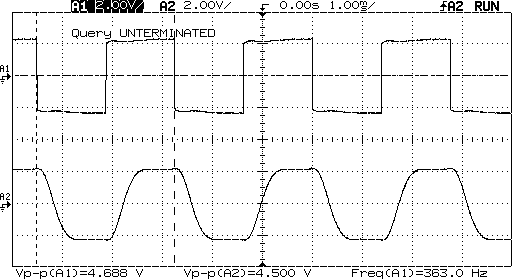
\includegraphics[width=.8\textwidth]{img/shot/squareWaveShot.png}
	\parbox{.6\textwidth}{
	\caption[Measured Step Response]{Results of the step response for a
	square wave input, as measured by an oscilloscope.  In this screenshot, the
	upper signal~(A1) is the input, while the lower~(A2) is the output.}
	\label{f:stepReal}}
\end{figure}
%
While there are similarities between the two resulting output signals, it is
significant to note that the simulated response exhibits Gibbs phenomena on the
leading transition of every wave, while the measured output does not show any
effects of Gibbs' phenomena, in fact failing to exceed the amplitude of the
input.

\subsection{Frequency Response}
\begin{figure}[H]
	\centering
	\begin{tikzpicture}[gnuplot]
%% generated with GNUPLOT 4.4p2 (Lua 5.1.4; terminal rev. 97, script rev. 96a)
%% Mon 28 Nov 2011 10:15:02 AM EST
\gpsolidlines
\gpcolor{gp lt color axes}
\gpsetlinetype{gp lt axes}
\gpsetlinewidth{1.00}
\draw[gp path] (1.504,0.985)--(10.242,0.985);
\gpcolor{gp lt color border}
\gpsetlinetype{gp lt border}
\draw[gp path] (1.504,0.985)--(1.684,0.985);
\node[gp node right] at (1.320,0.985) {-120};
\gpcolor{gp lt color axes}
\gpsetlinetype{gp lt axes}
\draw[gp path] (1.504,1.302)--(10.242,1.302);
\gpcolor{gp lt color border}
\gpsetlinetype{gp lt border}
\draw[gp path] (1.504,1.302)--(1.684,1.302);
\node[gp node right] at (1.320,1.302) {-110};
\gpcolor{gp lt color axes}
\gpsetlinetype{gp lt axes}
\draw[gp path] (1.504,1.619)--(10.242,1.619);
\gpcolor{gp lt color border}
\gpsetlinetype{gp lt border}
\draw[gp path] (1.504,1.619)--(1.684,1.619);
\node[gp node right] at (1.320,1.619) {-100};
\gpcolor{gp lt color axes}
\gpsetlinetype{gp lt axes}
\draw[gp path] (1.504,1.936)--(10.242,1.936);
\gpcolor{gp lt color border}
\gpsetlinetype{gp lt border}
\draw[gp path] (1.504,1.936)--(1.684,1.936);
\node[gp node right] at (1.320,1.936) {-90};
\gpcolor{gp lt color axes}
\gpsetlinetype{gp lt axes}
\draw[gp path] (1.504,2.253)--(10.242,2.253);
\gpcolor{gp lt color border}
\gpsetlinetype{gp lt border}
\draw[gp path] (1.504,2.253)--(1.684,2.253);
\node[gp node right] at (1.320,2.253) {-80};
\gpcolor{gp lt color axes}
\gpsetlinetype{gp lt axes}
\draw[gp path] (1.504,2.570)--(10.242,2.570);
\gpcolor{gp lt color border}
\gpsetlinetype{gp lt border}
\draw[gp path] (1.504,2.570)--(1.684,2.570);
\node[gp node right] at (1.320,2.570) {-70};
\gpcolor{gp lt color axes}
\gpsetlinetype{gp lt axes}
\draw[gp path] (1.504,2.888)--(10.242,2.888);
\gpcolor{gp lt color border}
\gpsetlinetype{gp lt border}
\draw[gp path] (1.504,2.888)--(1.684,2.888);
\node[gp node right] at (1.320,2.888) {-60};
\gpcolor{gp lt color axes}
\gpsetlinetype{gp lt axes}
\draw[gp path] (1.504,3.205)--(10.242,3.205);
\gpcolor{gp lt color border}
\gpsetlinetype{gp lt border}
\draw[gp path] (1.504,3.205)--(1.684,3.205);
\node[gp node right] at (1.320,3.205) {-50};
\gpcolor{gp lt color axes}
\gpsetlinetype{gp lt axes}
\draw[gp path] (1.504,3.522)--(10.242,3.522);
\gpcolor{gp lt color border}
\gpsetlinetype{gp lt border}
\draw[gp path] (1.504,3.522)--(1.684,3.522);
\node[gp node right] at (1.320,3.522) {-40};
\gpcolor{gp lt color axes}
\gpsetlinetype{gp lt axes}
\draw[gp path] (1.504,3.839)--(10.242,3.839);
\gpcolor{gp lt color border}
\gpsetlinetype{gp lt border}
\draw[gp path] (1.504,3.839)--(1.684,3.839);
\node[gp node right] at (1.320,3.839) {-30};
\gpcolor{gp lt color axes}
\gpsetlinetype{gp lt axes}
\draw[gp path] (1.504,4.156)--(10.242,4.156);
\gpcolor{gp lt color border}
\gpsetlinetype{gp lt border}
\draw[gp path] (1.504,4.156)--(1.684,4.156);
\node[gp node right] at (1.320,4.156) {-20};
\gpcolor{gp lt color axes}
\gpsetlinetype{gp lt axes}
\draw[gp path] (1.504,4.473)--(10.242,4.473);
\gpcolor{gp lt color border}
\gpsetlinetype{gp lt border}
\draw[gp path] (1.504,4.473)--(1.684,4.473);
\node[gp node right] at (1.320,4.473) {-10};
\gpcolor{gp lt color axes}
\gpsetlinetype{gp lt axes}
\draw[gp path] (1.504,4.790)--(10.242,4.790);
\gpcolor{gp lt color border}
\gpsetlinetype{gp lt border}
\draw[gp path] (1.504,4.790)--(1.684,4.790);
\node[gp node right] at (1.320,4.790) { 0};
\gpcolor{gp lt color axes}
\gpsetlinetype{gp lt axes}
\draw[gp path] (1.504,0.985)--(1.504,4.790);
\gpcolor{gp lt color border}
\gpsetlinetype{gp lt border}
\draw[gp path] (1.504,0.985)--(1.504,1.165);
\node[gp node center] at (1.504,0.677) { 1};
\gpcolor{gp lt color axes}
\gpsetlinetype{gp lt axes}
\draw[gp path] (2.338,0.985)--(2.338,4.790);
\gpcolor{gp lt color border}
\gpsetlinetype{gp lt border}
\draw[gp path] (2.338,0.985)--(2.338,1.165);
\node[gp node center] at (2.338,0.677) { 3};
\gpcolor{gp lt color axes}
\gpsetlinetype{gp lt axes}
\draw[gp path] (3.252,0.985)--(3.252,4.790);
\gpcolor{gp lt color border}
\gpsetlinetype{gp lt border}
\draw[gp path] (3.252,0.985)--(3.252,1.165);
\node[gp node center] at (3.252,0.677) { 10};
\gpcolor{gp lt color axes}
\gpsetlinetype{gp lt axes}
\draw[gp path] (4.085,0.985)--(4.085,4.790);
\gpcolor{gp lt color border}
\gpsetlinetype{gp lt border}
\draw[gp path] (4.085,0.985)--(4.085,1.165);
\node[gp node center] at (4.085,0.677) { 30};
\gpcolor{gp lt color axes}
\gpsetlinetype{gp lt axes}
\draw[gp path] (4.999,0.985)--(4.999,4.790);
\gpcolor{gp lt color border}
\gpsetlinetype{gp lt border}
\draw[gp path] (4.999,0.985)--(4.999,1.165);
\node[gp node center] at (4.999,0.677) { 100};
\gpcolor{gp lt color axes}
\gpsetlinetype{gp lt axes}
\draw[gp path] (5.833,0.985)--(5.833,4.790);
\gpcolor{gp lt color border}
\gpsetlinetype{gp lt border}
\draw[gp path] (5.833,0.985)--(5.833,1.165);
\node[gp node center] at (5.833,0.677) { 300};
\gpcolor{gp lt color axes}
\gpsetlinetype{gp lt axes}
\draw[gp path] (6.747,0.985)--(6.747,4.790);
\gpcolor{gp lt color border}
\gpsetlinetype{gp lt border}
\draw[gp path] (6.747,0.985)--(6.747,1.165);
\node[gp node center] at (6.747,0.677) { 1000};
\gpcolor{gp lt color axes}
\gpsetlinetype{gp lt axes}
\draw[gp path] (7.581,0.985)--(7.581,4.790);
\gpcolor{gp lt color border}
\gpsetlinetype{gp lt border}
\draw[gp path] (7.581,0.985)--(7.581,1.165);
\node[gp node center] at (7.581,0.677) { 3000};
\gpcolor{gp lt color axes}
\gpsetlinetype{gp lt axes}
\draw[gp path] (8.494,0.985)--(8.494,4.790);
\gpcolor{gp lt color border}
\gpsetlinetype{gp lt border}
\draw[gp path] (8.494,0.985)--(8.494,1.165);
\node[gp node center] at (8.494,0.677) { 10000};
\gpcolor{gp lt color axes}
\gpsetlinetype{gp lt axes}
\draw[gp path] (9.328,0.985)--(9.328,4.790);
\gpcolor{gp lt color border}
\gpsetlinetype{gp lt border}
\draw[gp path] (9.328,0.985)--(9.328,1.165);
\node[gp node center] at (9.328,0.677) { 30000};
\gpcolor{gp lt color axes}
\gpsetlinetype{gp lt axes}
\draw[gp path] (10.242,0.985)--(10.242,4.790);
\gpcolor{gp lt color border}
\gpsetlinetype{gp lt border}
\draw[gp path] (10.242,0.985)--(10.242,1.165);
\node[gp node center] at (10.242,0.677) { 100000};
\draw[gp path] (1.504,4.790)--(1.504,0.985)--(10.242,0.985)--(10.242,4.790)--cycle;
\node[gp node center,rotate=-270] at (0.246,2.887) {Output Gain, $A$, (\si{\decibel})};
\node[gp node center] at (5.873,0.215) {Input Frequency, $f$ (\si{\hertz})};
\node[gp node center] at (5.873,5.252) {Simulated Frequency Response of Third-order Low Pass Filter};
\gpcolor{gp lt color 0}
\gpsetlinetype{gp lt plot 0}
\gpsetlinewidth{3.00}
\draw[gp path] (1.504,4.790)--(1.511,4.790)--(1.518,4.790)--(1.525,4.790)--(1.532,4.790)%
  --(1.539,4.790)--(1.546,4.790)--(1.553,4.790)--(1.560,4.790)--(1.567,4.790)--(1.574,4.790)%
  --(1.581,4.790)--(1.588,4.790)--(1.595,4.790)--(1.602,4.790)--(1.609,4.790)--(1.616,4.790)%
  --(1.623,4.790)--(1.630,4.790)--(1.637,4.790)--(1.644,4.790)--(1.651,4.790)--(1.658,4.790)%
  --(1.665,4.790)--(1.672,4.790)--(1.679,4.790)--(1.686,4.790)--(1.693,4.790)--(1.700,4.790)%
  --(1.707,4.790)--(1.714,4.790)--(1.721,4.790)--(1.728,4.790)--(1.735,4.790)--(1.742,4.790)%
  --(1.749,4.790)--(1.756,4.790)--(1.763,4.790)--(1.770,4.790)--(1.777,4.790)--(1.784,4.790)%
  --(1.791,4.790)--(1.798,4.790)--(1.805,4.790)--(1.812,4.790)--(1.819,4.790)--(1.826,4.790)%
  --(1.833,4.790)--(1.840,4.790)--(1.847,4.790)--(1.854,4.790)--(1.861,4.790)--(1.868,4.790)%
  --(1.874,4.790)--(1.881,4.790)--(1.888,4.790)--(1.895,4.790)--(1.902,4.790)--(1.909,4.790)%
  --(1.916,4.790)--(1.923,4.790)--(1.930,4.790)--(1.937,4.790)--(1.944,4.790)--(1.951,4.790)%
  --(1.958,4.790)--(1.965,4.790)--(1.972,4.790)--(1.979,4.790)--(1.986,4.790)--(1.993,4.790)%
  --(2.000,4.790)--(2.007,4.790)--(2.014,4.790)--(2.021,4.790)--(2.028,4.790)--(2.035,4.790)%
  --(2.042,4.790)--(2.049,4.790)--(2.056,4.790)--(2.063,4.790)--(2.070,4.790)--(2.077,4.790)%
  --(2.084,4.790)--(2.091,4.790)--(2.098,4.790)--(2.105,4.790)--(2.112,4.790)--(2.119,4.790)%
  --(2.126,4.790)--(2.133,4.790)--(2.140,4.790)--(2.147,4.790)--(2.154,4.790)--(2.161,4.790)%
  --(2.168,4.790)--(2.175,4.790)--(2.182,4.790)--(2.189,4.790)--(2.196,4.790)--(2.203,4.790)%
  --(2.210,4.790)--(2.217,4.790)--(2.224,4.790)--(2.231,4.790)--(2.238,4.790)--(2.245,4.790)%
  --(2.252,4.790)--(2.259,4.790)--(2.266,4.790)--(2.273,4.790)--(2.280,4.790)--(2.287,4.790)%
  --(2.294,4.790)--(2.301,4.790)--(2.308,4.790)--(2.315,4.790)--(2.322,4.790)--(2.329,4.790)%
  --(2.336,4.790)--(2.343,4.790)--(2.350,4.790)--(2.357,4.790)--(2.364,4.790)--(2.371,4.790)%
  --(2.378,4.790)--(2.385,4.790)--(2.392,4.790)--(2.399,4.790)--(2.406,4.790)--(2.413,4.790)%
  --(2.420,4.790)--(2.427,4.790)--(2.434,4.790)--(2.441,4.790)--(2.448,4.790)--(2.455,4.790)%
  --(2.462,4.790)--(2.469,4.790)--(2.476,4.790)--(2.483,4.790)--(2.490,4.790)--(2.497,4.790)%
  --(2.504,4.790)--(2.511,4.790)--(2.518,4.790)--(2.525,4.790)--(2.532,4.790)--(2.539,4.790)%
  --(2.546,4.790)--(2.553,4.790)--(2.560,4.790)--(2.567,4.790)--(2.574,4.790)--(2.581,4.790)%
  --(2.588,4.790)--(2.595,4.790)--(2.601,4.790)--(2.608,4.790)--(2.615,4.790)--(2.622,4.790)%
  --(2.629,4.790)--(2.636,4.790)--(2.643,4.790)--(2.650,4.790)--(2.657,4.790)--(2.664,4.790)%
  --(2.671,4.790)--(2.678,4.790)--(2.685,4.790)--(2.692,4.790)--(2.699,4.790)--(2.706,4.790)%
  --(2.713,4.790)--(2.720,4.790)--(2.727,4.790)--(2.734,4.790)--(2.741,4.790)--(2.748,4.790)%
  --(2.755,4.790)--(2.762,4.790)--(2.769,4.790)--(2.776,4.790)--(2.783,4.790)--(2.790,4.790)%
  --(2.797,4.790)--(2.804,4.790)--(2.811,4.790)--(2.818,4.790)--(2.825,4.790)--(2.832,4.790)%
  --(2.839,4.790)--(2.846,4.790)--(2.853,4.790)--(2.860,4.790)--(2.867,4.790)--(2.874,4.790)%
  --(2.881,4.790)--(2.888,4.790)--(2.895,4.790)--(2.902,4.790)--(2.909,4.790)--(2.916,4.790)%
  --(2.923,4.790)--(2.930,4.790)--(2.937,4.790)--(2.944,4.790)--(2.951,4.790)--(2.958,4.790)%
  --(2.965,4.790)--(2.972,4.790)--(2.979,4.790)--(2.986,4.790)--(2.993,4.790)--(3.000,4.790)%
  --(3.007,4.790)--(3.014,4.790)--(3.021,4.790)--(3.028,4.790)--(3.035,4.790)--(3.042,4.790)%
  --(3.049,4.790)--(3.056,4.790)--(3.063,4.790)--(3.070,4.790)--(3.077,4.790)--(3.084,4.790)%
  --(3.091,4.790)--(3.098,4.790)--(3.105,4.790)--(3.112,4.790)--(3.119,4.790)--(3.126,4.790)%
  --(3.133,4.790)--(3.140,4.790)--(3.147,4.790)--(3.154,4.790)--(3.161,4.790)--(3.168,4.790)%
  --(3.175,4.790)--(3.182,4.790)--(3.189,4.790)--(3.196,4.790)--(3.203,4.790)--(3.210,4.790)%
  --(3.217,4.790)--(3.224,4.790)--(3.231,4.790)--(3.238,4.790)--(3.245,4.790)--(3.252,4.790)%
  --(3.259,4.790)--(3.266,4.790)--(3.273,4.790)--(3.280,4.790)--(3.287,4.790)--(3.294,4.790)%
  --(3.301,4.790)--(3.308,4.790)--(3.315,4.790)--(3.322,4.790)--(3.328,4.790)--(3.335,4.790)%
  --(3.342,4.790)--(3.349,4.790)--(3.356,4.790)--(3.363,4.790)--(3.370,4.790)--(3.377,4.790)%
  --(3.384,4.790)--(3.391,4.790)--(3.398,4.790)--(3.405,4.790)--(3.412,4.790)--(3.419,4.790)%
  --(3.426,4.790)--(3.433,4.790)--(3.440,4.790)--(3.447,4.790)--(3.454,4.790)--(3.461,4.790)%
  --(3.468,4.790)--(3.475,4.790)--(3.482,4.790)--(3.489,4.790)--(3.496,4.790)--(3.503,4.790)%
  --(3.510,4.790)--(3.517,4.790)--(3.524,4.790)--(3.531,4.790)--(3.538,4.790)--(3.545,4.790)%
  --(3.552,4.790)--(3.559,4.790)--(3.566,4.790)--(3.573,4.790)--(3.580,4.790)--(3.587,4.790)%
  --(3.594,4.790)--(3.601,4.790)--(3.608,4.790)--(3.615,4.790)--(3.622,4.790)--(3.629,4.790)%
  --(3.636,4.790)--(3.643,4.790)--(3.650,4.790)--(3.657,4.790)--(3.664,4.790)--(3.671,4.790)%
  --(3.678,4.790)--(3.685,4.790)--(3.692,4.790)--(3.699,4.790)--(3.706,4.790)--(3.713,4.790)%
  --(3.720,4.790)--(3.727,4.790)--(3.734,4.790)--(3.741,4.790)--(3.748,4.790)--(3.755,4.790)%
  --(3.762,4.790)--(3.769,4.790)--(3.776,4.790)--(3.783,4.790)--(3.790,4.790)--(3.797,4.790)%
  --(3.804,4.790)--(3.811,4.790)--(3.818,4.790)--(3.825,4.790)--(3.832,4.790)--(3.839,4.790)%
  --(3.846,4.790)--(3.853,4.790)--(3.860,4.790)--(3.867,4.790)--(3.874,4.790)--(3.881,4.790)%
  --(3.888,4.790)--(3.895,4.790)--(3.902,4.790)--(3.909,4.790)--(3.916,4.790)--(3.923,4.790)%
  --(3.930,4.790)--(3.937,4.790)--(3.944,4.790)--(3.951,4.790)--(3.958,4.790)--(3.965,4.790)%
  --(3.972,4.790)--(3.979,4.790)--(3.986,4.790)--(3.993,4.790)--(4.000,4.790)--(4.007,4.790)%
  --(4.014,4.790)--(4.021,4.790)--(4.028,4.790)--(4.035,4.790)--(4.042,4.790)--(4.049,4.790)%
  --(4.055,4.790)--(4.062,4.790)--(4.069,4.790)--(4.076,4.790)--(4.083,4.790)--(4.090,4.790)%
  --(4.097,4.790)--(4.104,4.790)--(4.111,4.790)--(4.118,4.790)--(4.125,4.790)--(4.132,4.790)%
  --(4.139,4.790)--(4.146,4.790)--(4.153,4.790)--(4.160,4.790)--(4.167,4.790)--(4.174,4.790)%
  --(4.181,4.790)--(4.188,4.790)--(4.195,4.790)--(4.202,4.790)--(4.209,4.790)--(4.216,4.790)%
  --(4.223,4.790)--(4.230,4.790)--(4.237,4.790)--(4.244,4.790)--(4.251,4.790)--(4.258,4.790)%
  --(4.265,4.790)--(4.272,4.790)--(4.279,4.790)--(4.286,4.790)--(4.293,4.790)--(4.300,4.790)%
  --(4.307,4.790)--(4.314,4.790)--(4.321,4.790)--(4.328,4.790)--(4.335,4.790)--(4.342,4.790)%
  --(4.349,4.790)--(4.356,4.790)--(4.363,4.790)--(4.370,4.790)--(4.377,4.790)--(4.384,4.790)%
  --(4.391,4.790)--(4.398,4.790)--(4.405,4.790)--(4.412,4.790)--(4.419,4.790)--(4.426,4.790)%
  --(4.433,4.790)--(4.440,4.790)--(4.447,4.790)--(4.454,4.790)--(4.461,4.790)--(4.468,4.790)%
  --(4.475,4.790)--(4.482,4.790)--(4.489,4.790)--(4.496,4.790)--(4.503,4.790)--(4.510,4.790)%
  --(4.517,4.790)--(4.524,4.790)--(4.531,4.790)--(4.538,4.790)--(4.545,4.790)--(4.552,4.790)%
  --(4.559,4.790)--(4.566,4.790)--(4.573,4.790)--(4.580,4.790)--(4.587,4.790)--(4.594,4.790)%
  --(4.601,4.790)--(4.608,4.790)--(4.615,4.790)--(4.622,4.790)--(4.629,4.790)--(4.636,4.790)%
  --(4.643,4.790)--(4.650,4.790)--(4.657,4.790)--(4.664,4.790)--(4.671,4.790)--(4.678,4.790)%
  --(4.685,4.790)--(4.692,4.790)--(4.699,4.790)--(4.706,4.790)--(4.713,4.790)--(4.720,4.789)%
  --(4.727,4.789)--(4.734,4.789)--(4.741,4.789)--(4.748,4.789)--(4.755,4.789)--(4.762,4.789)%
  --(4.769,4.789)--(4.776,4.789)--(4.782,4.789)--(4.789,4.789)--(4.796,4.789)--(4.803,4.789)%
  --(4.810,4.789)--(4.817,4.789)--(4.824,4.789)--(4.831,4.789)--(4.838,4.789)--(4.845,4.789)%
  --(4.852,4.789)--(4.859,4.789)--(4.866,4.789)--(4.873,4.789)--(4.880,4.789)--(4.887,4.789)%
  --(4.894,4.789)--(4.901,4.789)--(4.908,4.789)--(4.915,4.789)--(4.922,4.789)--(4.929,4.789)%
  --(4.936,4.789)--(4.943,4.789)--(4.950,4.789)--(4.957,4.789)--(4.964,4.789)--(4.971,4.789)%
  --(4.978,4.789)--(4.985,4.789)--(4.992,4.789)--(4.999,4.789)--(5.006,4.789)--(5.013,4.789)%
  --(5.020,4.789)--(5.027,4.789)--(5.034,4.789)--(5.041,4.789)--(5.048,4.789)--(5.055,4.789)%
  --(5.062,4.789)--(5.069,4.789)--(5.076,4.789)--(5.083,4.789)--(5.090,4.789)--(5.097,4.789)%
  --(5.104,4.789)--(5.111,4.789)--(5.118,4.789)--(5.125,4.789)--(5.132,4.789)--(5.139,4.788)%
  --(5.146,4.788)--(5.153,4.788)--(5.160,4.788)--(5.167,4.788)--(5.174,4.788)--(5.181,4.788)%
  --(5.188,4.788)--(5.195,4.788)--(5.202,4.788)--(5.209,4.788)--(5.216,4.788)--(5.223,4.788)%
  --(5.230,4.788)--(5.237,4.788)--(5.244,4.788)--(5.251,4.788)--(5.258,4.788)--(5.265,4.788)%
  --(5.272,4.788)--(5.279,4.788)--(5.286,4.788)--(5.293,4.788)--(5.300,4.788)--(5.307,4.788)%
  --(5.314,4.788)--(5.321,4.788)--(5.328,4.787)--(5.335,4.787)--(5.342,4.787)--(5.349,4.787)%
  --(5.356,4.787)--(5.363,4.787)--(5.370,4.787)--(5.377,4.787)--(5.384,4.787)--(5.391,4.787)%
  --(5.398,4.787)--(5.405,4.787)--(5.412,4.787)--(5.419,4.787)--(5.426,4.787)--(5.433,4.787)%
  --(5.440,4.787)--(5.447,4.787)--(5.454,4.787)--(5.461,4.786)--(5.468,4.786)--(5.475,4.786)%
  --(5.482,4.786)--(5.489,4.786)--(5.496,4.786)--(5.503,4.786)--(5.509,4.786)--(5.516,4.786)%
  --(5.523,4.786)--(5.530,4.786)--(5.537,4.786)--(5.544,4.786)--(5.551,4.786)--(5.558,4.785)%
  --(5.565,4.785)--(5.572,4.785)--(5.579,4.785)--(5.586,4.785)--(5.593,4.785)--(5.600,4.785)%
  --(5.607,4.785)--(5.614,4.785)--(5.621,4.785)--(5.628,4.785)--(5.635,4.784)--(5.642,4.784)%
  --(5.649,4.784)--(5.656,4.784)--(5.663,4.784)--(5.670,4.784)--(5.677,4.784)--(5.684,4.784)%
  --(5.691,4.784)--(5.698,4.783)--(5.705,4.783)--(5.712,4.783)--(5.719,4.783)--(5.726,4.783)%
  --(5.733,4.783)--(5.740,4.783)--(5.747,4.783)--(5.754,4.782)--(5.761,4.782)--(5.768,4.782)%
  --(5.775,4.782)--(5.782,4.782)--(5.789,4.782)--(5.796,4.782)--(5.803,4.781)--(5.810,4.781)%
  --(5.817,4.781)--(5.824,4.781)--(5.831,4.781)--(5.838,4.781)--(5.845,4.780)--(5.852,4.780)%
  --(5.859,4.780)--(5.866,4.780)--(5.873,4.780)--(5.880,4.780)--(5.887,4.779)--(5.894,4.779)%
  --(5.901,4.779)--(5.908,4.779)--(5.915,4.779)--(5.922,4.778)--(5.929,4.778)--(5.936,4.778)%
  --(5.943,4.778)--(5.950,4.778)--(5.957,4.777)--(5.964,4.777)--(5.971,4.777)--(5.978,4.777)%
  --(5.985,4.776)--(5.992,4.776)--(5.999,4.776)--(6.006,4.776)--(6.013,4.775)--(6.020,4.775)%
  --(6.027,4.775)--(6.034,4.775)--(6.041,4.774)--(6.048,4.774)--(6.055,4.774)--(6.062,4.773)%
  --(6.069,4.773)--(6.076,4.773)--(6.083,4.773)--(6.090,4.772)--(6.097,4.772)--(6.104,4.772)%
  --(6.111,4.771)--(6.118,4.771)--(6.125,4.771)--(6.132,4.770)--(6.139,4.770)--(6.146,4.769)%
  --(6.153,4.769)--(6.160,4.769)--(6.167,4.768)--(6.174,4.768)--(6.181,4.768)--(6.188,4.767)%
  --(6.195,4.767)--(6.202,4.766)--(6.209,4.766)--(6.216,4.765)--(6.223,4.765)--(6.230,4.764)%
  --(6.237,4.764)--(6.243,4.764)--(6.250,4.763)--(6.257,4.763)--(6.264,4.762)--(6.271,4.762)%
  --(6.278,4.761)--(6.285,4.761)--(6.292,4.760)--(6.299,4.759)--(6.306,4.759)--(6.313,4.758)%
  --(6.320,4.758)--(6.327,4.757)--(6.334,4.756)--(6.341,4.756)--(6.348,4.755)--(6.355,4.755)%
  --(6.362,4.754)--(6.369,4.753)--(6.376,4.752)--(6.383,4.752)--(6.390,4.751)--(6.397,4.750)%
  --(6.404,4.750)--(6.411,4.749)--(6.418,4.748)--(6.425,4.747)--(6.432,4.746)--(6.439,4.745)%
  --(6.446,4.745)--(6.453,4.744)--(6.460,4.743)--(6.467,4.742)--(6.474,4.741)--(6.481,4.740)%
  --(6.488,4.739)--(6.495,4.738)--(6.502,4.737)--(6.509,4.736)--(6.516,4.735)--(6.523,4.733)%
  --(6.530,4.732)--(6.537,4.731)--(6.544,4.730)--(6.551,4.729)--(6.558,4.727)--(6.565,4.726)%
  --(6.572,4.725)--(6.579,4.723)--(6.586,4.722)--(6.593,4.720)--(6.600,4.719)--(6.607,4.717)%
  --(6.614,4.716)--(6.621,4.714)--(6.628,4.712)--(6.635,4.711)--(6.642,4.709)--(6.649,4.707)%
  --(6.656,4.705)--(6.663,4.703)--(6.670,4.701)--(6.677,4.699)--(6.684,4.697)--(6.691,4.695)%
  --(6.698,4.693)--(6.705,4.691)--(6.712,4.689)--(6.719,4.686)--(6.726,4.684)--(6.733,4.681)%
  --(6.740,4.679)--(6.747,4.676)--(6.754,4.674)--(6.761,4.671)--(6.768,4.668)--(6.775,4.665)%
  --(6.782,4.662)--(6.789,4.659)--(6.796,4.656)--(6.803,4.653)--(6.810,4.650)--(6.817,4.647)%
  --(6.824,4.643)--(6.831,4.640)--(6.838,4.636)--(6.845,4.633)--(6.852,4.629)--(6.859,4.625)%
  --(6.866,4.621)--(6.873,4.617)--(6.880,4.614)--(6.887,4.609)--(6.894,4.605)--(6.901,4.601)%
  --(6.908,4.597)--(6.915,4.592)--(6.922,4.588)--(6.929,4.583)--(6.936,4.579)--(6.943,4.574)%
  --(6.950,4.569)--(6.957,4.564)--(6.964,4.559)--(6.970,4.554)--(6.977,4.549)--(6.984,4.544)%
  --(6.991,4.539)--(6.998,4.534)--(7.005,4.528)--(7.012,4.523)--(7.019,4.517)--(7.026,4.512)%
  --(7.033,4.506)--(7.040,4.501)--(7.047,4.495)--(7.054,4.489)--(7.061,4.483)--(7.068,4.477)%
  --(7.075,4.471)--(7.082,4.465)--(7.089,4.459)--(7.096,4.453)--(7.103,4.447)--(7.110,4.441)%
  --(7.117,4.434)--(7.124,4.428)--(7.131,4.421)--(7.138,4.415)--(7.145,4.409)--(7.152,4.402)%
  --(7.159,4.395)--(7.166,4.389)--(7.173,4.382)--(7.180,4.376)--(7.187,4.369)--(7.194,4.362)%
  --(7.201,4.355)--(7.208,4.348)--(7.215,4.342)--(7.222,4.335)--(7.229,4.328)--(7.236,4.321)%
  --(7.243,4.314)--(7.250,4.307)--(7.257,4.300)--(7.264,4.293)--(7.271,4.286)--(7.278,4.279)%
  --(7.285,4.272)--(7.292,4.265)--(7.299,4.257)--(7.306,4.250)--(7.313,4.243)--(7.320,4.236)%
  --(7.327,4.229)--(7.334,4.221)--(7.341,4.214)--(7.348,4.207)--(7.355,4.200)--(7.362,4.192)%
  --(7.369,4.185)--(7.376,4.178)--(7.383,4.170)--(7.390,4.163)--(7.397,4.156)--(7.404,4.148)%
  --(7.411,4.141)--(7.418,4.134)--(7.425,4.126)--(7.432,4.119)--(7.439,4.111)--(7.446,4.104)%
  --(7.453,4.097)--(7.460,4.089)--(7.467,4.082)--(7.474,4.074)--(7.481,4.067)--(7.488,4.059)%
  --(7.495,4.052)--(7.502,4.044)--(7.509,4.037)--(7.516,4.029)--(7.523,4.022)--(7.530,4.014)%
  --(7.537,4.007)--(7.544,3.999)--(7.551,3.992)--(7.558,3.984)--(7.565,3.977)--(7.572,3.969)%
  --(7.579,3.962)--(7.586,3.954)--(7.593,3.947)--(7.600,3.939)--(7.607,3.932)--(7.614,3.924)%
  --(7.621,3.916)--(7.628,3.909)--(7.635,3.901)--(7.642,3.894)--(7.649,3.886)--(7.656,3.879)%
  --(7.663,3.871)--(7.670,3.864)--(7.677,3.856)--(7.684,3.848)--(7.691,3.841)--(7.697,3.833)%
  --(7.704,3.826)--(7.711,3.818)--(7.718,3.811)--(7.725,3.803)--(7.732,3.795)--(7.739,3.788)%
  --(7.746,3.780)--(7.753,3.773)--(7.760,3.765)--(7.767,3.757)--(7.774,3.750)--(7.781,3.742)%
  --(7.788,3.735)--(7.795,3.727)--(7.802,3.719)--(7.809,3.712)--(7.816,3.704)--(7.823,3.697)%
  --(7.830,3.689)--(7.837,3.681)--(7.844,3.674)--(7.851,3.666)--(7.858,3.659)--(7.865,3.651)%
  --(7.872,3.643)--(7.879,3.636)--(7.886,3.628)--(7.893,3.621)--(7.900,3.613)--(7.907,3.605)%
  --(7.914,3.598)--(7.921,3.590)--(7.928,3.583)--(7.935,3.575)--(7.942,3.567)--(7.949,3.560)%
  --(7.956,3.552)--(7.963,3.545)--(7.970,3.537)--(7.977,3.529)--(7.984,3.522)--(7.991,3.514)%
  --(7.998,3.507)--(8.005,3.499)--(8.012,3.491)--(8.019,3.484)--(8.026,3.476)--(8.033,3.469)%
  --(8.040,3.461)--(8.047,3.453)--(8.054,3.446)--(8.061,3.438)--(8.068,3.430)--(8.075,3.423)%
  --(8.082,3.415)--(8.089,3.408)--(8.096,3.400)--(8.103,3.392)--(8.110,3.385)--(8.117,3.377)%
  --(8.124,3.370)--(8.131,3.362)--(8.138,3.354)--(8.145,3.347)--(8.152,3.339)--(8.159,3.332)%
  --(8.166,3.324)--(8.173,3.316)--(8.180,3.309)--(8.187,3.301)--(8.194,3.293)--(8.201,3.286)%
  --(8.208,3.278)--(8.215,3.271)--(8.222,3.263)--(8.229,3.255)--(8.236,3.248)--(8.243,3.240)%
  --(8.250,3.233)--(8.257,3.225)--(8.264,3.217)--(8.271,3.210)--(8.278,3.202)--(8.285,3.194)%
  --(8.292,3.187)--(8.299,3.179)--(8.306,3.172)--(8.313,3.164)--(8.320,3.156)--(8.327,3.149)%
  --(8.334,3.141)--(8.341,3.134)--(8.348,3.126)--(8.355,3.118)--(8.362,3.111)--(8.369,3.103)%
  --(8.376,3.096)--(8.383,3.088)--(8.390,3.080)--(8.397,3.073)--(8.404,3.065)--(8.411,3.057)%
  --(8.418,3.050)--(8.424,3.042)--(8.431,3.035)--(8.438,3.027)--(8.445,3.019)--(8.452,3.012)%
  --(8.459,3.004)--(8.466,2.997)--(8.473,2.989)--(8.480,2.981)--(8.487,2.974)--(8.494,2.966)%
  --(8.501,2.959)--(8.508,2.951)--(8.515,2.943)--(8.522,2.936)--(8.529,2.928)--(8.536,2.920)%
  --(8.543,2.913)--(8.550,2.905)--(8.557,2.898)--(8.564,2.890)--(8.571,2.882)--(8.578,2.875)%
  --(8.585,2.867)--(8.592,2.860)--(8.599,2.852)--(8.606,2.844)--(8.613,2.837)--(8.620,2.829)%
  --(8.627,2.822)--(8.634,2.814)--(8.641,2.806)--(8.648,2.799)--(8.655,2.791)--(8.662,2.783)%
  --(8.669,2.776)--(8.676,2.768)--(8.683,2.761)--(8.690,2.753)--(8.697,2.745)--(8.704,2.738)%
  --(8.711,2.730)--(8.718,2.723)--(8.725,2.715)--(8.732,2.707)--(8.739,2.700)--(8.746,2.692)%
  --(8.753,2.685)--(8.760,2.677)--(8.767,2.669)--(8.774,2.662)--(8.781,2.654)--(8.788,2.646)%
  --(8.795,2.639)--(8.802,2.631)--(8.809,2.624)--(8.816,2.616)--(8.823,2.608)--(8.830,2.601)%
  --(8.837,2.593)--(8.844,2.586)--(8.851,2.578)--(8.858,2.570)--(8.865,2.563)--(8.872,2.555)%
  --(8.879,2.548)--(8.886,2.540)--(8.893,2.532)--(8.900,2.525)--(8.907,2.517)--(8.914,2.509)%
  --(8.921,2.502)--(8.928,2.494)--(8.935,2.487)--(8.942,2.479)--(8.949,2.471)--(8.956,2.464)%
  --(8.963,2.456)--(8.970,2.449)--(8.977,2.441)--(8.984,2.433)--(8.991,2.426)--(8.998,2.418)%
  --(9.005,2.411)--(9.012,2.403)--(9.019,2.395)--(9.026,2.388)--(9.033,2.380)--(9.040,2.372)%
  --(9.047,2.365)--(9.054,2.357)--(9.061,2.350)--(9.068,2.342)--(9.075,2.334)--(9.082,2.327)%
  --(9.089,2.319)--(9.096,2.312)--(9.103,2.304)--(9.110,2.296)--(9.117,2.289)--(9.124,2.281)%
  --(9.131,2.274)--(9.138,2.266)--(9.145,2.258)--(9.151,2.251)--(9.158,2.243)--(9.165,2.235)%
  --(9.172,2.228)--(9.179,2.220)--(9.186,2.213)--(9.193,2.205)--(9.200,2.197)--(9.207,2.190)%
  --(9.214,2.182)--(9.221,2.175)--(9.228,2.167)--(9.235,2.159)--(9.242,2.152)--(9.249,2.144)%
  --(9.256,2.137)--(9.263,2.129)--(9.270,2.121)--(9.277,2.114)--(9.284,2.106)--(9.291,2.099)%
  --(9.298,2.091)--(9.305,2.083)--(9.312,2.076)--(9.319,2.068)--(9.326,2.060)--(9.333,2.053)%
  --(9.340,2.045)--(9.347,2.038)--(9.354,2.030)--(9.361,2.022)--(9.368,2.015)--(9.375,2.007)%
  --(9.382,2.000)--(9.389,1.992)--(9.396,1.984)--(9.403,1.977)--(9.410,1.969)--(9.417,1.962)%
  --(9.424,1.954)--(9.431,1.946)--(9.438,1.939)--(9.445,1.931)--(9.452,1.923)--(9.459,1.916)%
  --(9.466,1.908)--(9.473,1.901)--(9.480,1.893)--(9.487,1.885)--(9.494,1.878)--(9.501,1.870)%
  --(9.508,1.863)--(9.515,1.855)--(9.522,1.847)--(9.529,1.840)--(9.536,1.832)--(9.543,1.825)%
  --(9.550,1.817)--(9.557,1.809)--(9.564,1.802)--(9.571,1.794)--(9.578,1.786)--(9.585,1.779)%
  --(9.592,1.771)--(9.599,1.764)--(9.606,1.756)--(9.613,1.748)--(9.620,1.741)--(9.627,1.733)%
  --(9.634,1.726)--(9.641,1.718)--(9.648,1.710)--(9.655,1.703)--(9.662,1.695)--(9.669,1.688)%
  --(9.676,1.680)--(9.683,1.672)--(9.690,1.665)--(9.697,1.657)--(9.704,1.650)--(9.711,1.642)%
  --(9.718,1.634)--(9.725,1.627)--(9.732,1.619)--(9.739,1.611)--(9.746,1.604)--(9.753,1.596)%
  --(9.760,1.589)--(9.767,1.581)--(9.774,1.573)--(9.781,1.566)--(9.788,1.558)--(9.795,1.551)%
  --(9.802,1.543)--(9.809,1.535)--(9.816,1.528)--(9.823,1.520)--(9.830,1.513)--(9.837,1.505)%
  --(9.844,1.497)--(9.851,1.490)--(9.858,1.482)--(9.865,1.474)--(9.872,1.467)--(9.878,1.459)%
  --(9.885,1.452)--(9.892,1.444)--(9.899,1.436)--(9.906,1.429)--(9.913,1.421)--(9.920,1.414)%
  --(9.927,1.406)--(9.934,1.398)--(9.941,1.391)--(9.948,1.383)--(9.955,1.376)--(9.962,1.368)%
  --(9.969,1.360)--(9.976,1.353)--(9.983,1.345)--(9.990,1.337)--(9.997,1.330)--(10.004,1.322)%
  --(10.011,1.315)--(10.018,1.307)--(10.025,1.299)--(10.032,1.292)--(10.039,1.284)--(10.046,1.277)%
  --(10.053,1.269)--(10.060,1.261)--(10.067,1.254)--(10.074,1.246)--(10.081,1.239)--(10.088,1.231)%
  --(10.095,1.223)--(10.102,1.216)--(10.109,1.208)--(10.116,1.201)--(10.123,1.193)--(10.130,1.185)%
  --(10.137,1.178)--(10.144,1.170)--(10.151,1.162)--(10.158,1.155)--(10.165,1.147)--(10.172,1.140)%
  --(10.179,1.132)--(10.186,1.124)--(10.193,1.117)--(10.200,1.109)--(10.207,1.102)--(10.214,1.094)%
  --(10.221,1.086)--(10.228,1.079)--(10.235,1.071)--(10.242,1.064);
\gpcolor{gp lt color border}
\gpsetlinetype{gp lt border}
\gpsetlinewidth{1.00}
\draw[gp path] (1.504,4.790)--(1.504,0.985)--(10.242,0.985)--(10.242,4.790)--cycle;
%% coordinates of the plot area
\gpdefrectangularnode{gp plot 1}{\pgfpoint{1.504cm}{0.985cm}}{\pgfpoint{10.242cm}{4.790cm}}
\end{tikzpicture}
%% gnuplot variables

\end{figure}

\begin{figure}[H]
	\centering
	\begin{tikzpicture}[gnuplot]
%% generated with GNUPLOT 4.4p2 (Lua 5.1.4; terminal rev. 97, script rev. 96a)
%% Mon 28 Nov 2011 10:15:02 AM EST
\gpsolidlines
\gpcolor{gp lt color axes}
\gpsetlinetype{gp lt axes}
\gpsetlinewidth{1.00}
\draw[gp path] (1.320,0.985)--(10.242,0.985);
\gpcolor{gp lt color border}
\gpsetlinetype{gp lt border}
\draw[gp path] (1.320,0.985)--(1.500,0.985);
\node[gp node right] at (1.136,0.985) {-40};
\gpcolor{gp lt color axes}
\gpsetlinetype{gp lt axes}
\draw[gp path] (1.320,1.936)--(10.242,1.936);
\gpcolor{gp lt color border}
\gpsetlinetype{gp lt border}
\draw[gp path] (1.320,1.936)--(1.500,1.936);
\node[gp node right] at (1.136,1.936) {-30};
\gpcolor{gp lt color axes}
\gpsetlinetype{gp lt axes}
\draw[gp path] (1.320,2.888)--(10.242,2.888);
\gpcolor{gp lt color border}
\gpsetlinetype{gp lt border}
\draw[gp path] (1.320,2.888)--(1.500,2.888);
\node[gp node right] at (1.136,2.888) {-20};
\gpcolor{gp lt color axes}
\gpsetlinetype{gp lt axes}
\draw[gp path] (1.320,3.839)--(10.242,3.839);
\gpcolor{gp lt color border}
\gpsetlinetype{gp lt border}
\draw[gp path] (1.320,3.839)--(1.500,3.839);
\node[gp node right] at (1.136,3.839) {-10};
\gpcolor{gp lt color axes}
\gpsetlinetype{gp lt axes}
\draw[gp path] (1.320,4.790)--(10.242,4.790);
\gpcolor{gp lt color border}
\gpsetlinetype{gp lt border}
\draw[gp path] (1.320,4.790)--(1.500,4.790);
\node[gp node right] at (1.136,4.790) { 0};
\gpcolor{gp lt color axes}
\gpsetlinetype{gp lt axes}
\draw[gp path] (2.458,0.985)--(2.458,4.790);
\gpcolor{gp lt color border}
\gpsetlinetype{gp lt border}
\draw[gp path] (2.458,0.985)--(2.458,1.165);
\node[gp node center] at (2.458,0.677) { 100};
\gpcolor{gp lt color axes}
\gpsetlinetype{gp lt axes}
\draw[gp path] (4.315,0.985)--(4.315,4.790);
\gpcolor{gp lt color border}
\gpsetlinetype{gp lt border}
\draw[gp path] (4.315,0.985)--(4.315,1.165);
\node[gp node center] at (4.315,0.677) { 300};
\gpcolor{gp lt color axes}
\gpsetlinetype{gp lt axes}
\draw[gp path] (6.350,0.985)--(6.350,4.790);
\gpcolor{gp lt color border}
\gpsetlinetype{gp lt border}
\draw[gp path] (6.350,0.985)--(6.350,1.165);
\node[gp node center] at (6.350,0.677) { 1000};
\gpcolor{gp lt color axes}
\gpsetlinetype{gp lt axes}
\draw[gp path] (8.207,0.985)--(8.207,4.790);
\gpcolor{gp lt color border}
\gpsetlinetype{gp lt border}
\draw[gp path] (8.207,0.985)--(8.207,1.165);
\node[gp node center] at (8.207,0.677) { 3000};
\gpcolor{gp lt color axes}
\gpsetlinetype{gp lt axes}
\draw[gp path] (10.242,0.985)--(10.242,4.790);
\gpcolor{gp lt color border}
\gpsetlinetype{gp lt border}
\draw[gp path] (10.242,0.985)--(10.242,1.165);
\node[gp node center] at (10.242,0.677) { 10000};
\draw[gp path] (1.320,4.790)--(1.320,0.985)--(10.242,0.985)--(10.242,4.790)--cycle;
\node[gp node center,rotate=-270] at (0.246,2.887) {Output Gain, $A$, (\si{\decibel})};
\node[gp node center] at (5.781,0.215) {Input Frequency, $f$ (\si{\hertz})};
\node[gp node center] at (5.781,5.252) {Measured Frequency Response of Third-order Low Pass Filter};
\gpcolor{gp lt color 0}
\gpsetlinetype{gp lt plot 0}
\gpsetlinewidth{3.00}
\draw[gp path] (1.320,4.779)--(1.502,4.768)--(1.684,4.779)--(1.866,4.769)--(2.048,4.768)%
  --(2.230,4.779)--(2.412,4.758)--(2.595,4.768)--(2.777,4.768)--(2.959,4.758)--(3.141,4.768)%
  --(3.323,4.757)--(3.505,4.768)--(3.687,4.747)--(3.869,4.768)--(4.051,4.745)--(4.233,4.745)%
  --(4.415,4.722)--(4.597,4.710)--(4.780,4.709)--(4.962,4.695)--(5.144,4.695)--(5.326,4.659)%
  --(5.508,4.644)--(5.690,4.628)--(5.872,4.589)--(6.054,4.541)--(6.236,4.486)--(6.418,4.377)%
  --(6.600,4.271)--(6.782,4.124)--(6.965,3.935)--(7.147,3.727)--(7.329,3.505)--(7.511,3.293)%
  --(7.693,3.038)--(7.875,2.854)--(8.057,2.585)--(8.239,2.400)--(8.421,2.220)--(8.603,2.117)%
  --(8.785,1.818)--(8.967,1.836)--(9.150,1.775)--(9.332,2.007)--(9.514,1.786)--(9.696,1.858)%
  --(9.878,1.818)--(10.060,1.731)--(10.242,1.818);
\gpcolor{gp lt color border}
\gpsetlinetype{gp lt border}
\gpsetlinewidth{1.00}
\draw[gp path] (1.320,4.790)--(1.320,0.985)--(10.242,0.985)--(10.242,4.790)--cycle;
%% coordinates of the plot area
\gpdefrectangularnode{gp plot 1}{\pgfpoint{1.320cm}{0.985cm}}{\pgfpoint{10.242cm}{4.790cm}}
\end{tikzpicture}
%% gnuplot variables

\end{figure}

\begin{figure}[H]
	\centering
	\begin{tikzpicture}[gnuplot]
%% generated with GNUPLOT 4.4p2 (Lua 5.1.4; terminal rev. 97, script rev. 96a)
%% Thu 24 Nov 2011 11:30:02 PM EST
\gpsolidlines
\gpcolor{gp lt color axes}
\gpsetlinetype{gp lt axes}
\gpsetlinewidth{1.00}
\draw[gp path] (1.320,0.985)--(10.242,0.985);
\gpcolor{gp lt color border}
\gpsetlinetype{gp lt border}
\draw[gp path] (1.320,0.985)--(1.500,0.985);
\node[gp node right] at (1.136,0.985) {-60};
\gpcolor{gp lt color axes}
\gpsetlinetype{gp lt axes}
\draw[gp path] (1.320,1.619)--(10.242,1.619);
\gpcolor{gp lt color border}
\gpsetlinetype{gp lt border}
\draw[gp path] (1.320,1.619)--(1.500,1.619);
\node[gp node right] at (1.136,1.619) {-50};
\gpcolor{gp lt color axes}
\gpsetlinetype{gp lt axes}
\draw[gp path] (1.320,2.253)--(10.242,2.253);
\gpcolor{gp lt color border}
\gpsetlinetype{gp lt border}
\draw[gp path] (1.320,2.253)--(1.500,2.253);
\node[gp node right] at (1.136,2.253) {-40};
\gpcolor{gp lt color axes}
\gpsetlinetype{gp lt axes}
\draw[gp path] (1.320,2.888)--(10.242,2.888);
\gpcolor{gp lt color border}
\gpsetlinetype{gp lt border}
\draw[gp path] (1.320,2.888)--(1.500,2.888);
\node[gp node right] at (1.136,2.888) {-30};
\gpcolor{gp lt color axes}
\gpsetlinetype{gp lt axes}
\draw[gp path] (1.320,3.522)--(10.242,3.522);
\gpcolor{gp lt color border}
\gpsetlinetype{gp lt border}
\draw[gp path] (1.320,3.522)--(1.500,3.522);
\node[gp node right] at (1.136,3.522) {-20};
\gpcolor{gp lt color axes}
\gpsetlinetype{gp lt axes}
\draw[gp path] (1.320,4.156)--(10.242,4.156);
\gpcolor{gp lt color border}
\gpsetlinetype{gp lt border}
\draw[gp path] (1.320,4.156)--(1.500,4.156);
\node[gp node right] at (1.136,4.156) {-10};
\gpcolor{gp lt color axes}
\gpsetlinetype{gp lt axes}
\draw[gp path] (1.320,4.790)--(10.242,4.790);
\gpcolor{gp lt color border}
\gpsetlinetype{gp lt border}
\draw[gp path] (1.320,4.790)--(1.500,4.790);
\node[gp node right] at (1.136,4.790) { 0};
\gpcolor{gp lt color axes}
\gpsetlinetype{gp lt axes}
\draw[gp path] (2.487,0.985)--(2.487,4.790);
\gpcolor{gp lt color border}
\gpsetlinetype{gp lt border}
\draw[gp path] (2.487,0.985)--(2.487,1.165);
\node[gp node center] at (2.487,0.677) { 100};
\gpcolor{gp lt color axes}
\gpsetlinetype{gp lt axes}
\draw[gp path] (4.337,0.985)--(4.337,4.790);
\gpcolor{gp lt color border}
\gpsetlinetype{gp lt border}
\draw[gp path] (4.337,0.985)--(4.337,1.165);
\node[gp node center] at (4.337,0.677) { 300};
\gpcolor{gp lt color axes}
\gpsetlinetype{gp lt axes}
\draw[gp path] (6.365,0.985)--(6.365,4.790);
\gpcolor{gp lt color border}
\gpsetlinetype{gp lt border}
\draw[gp path] (6.365,0.985)--(6.365,1.165);
\node[gp node center] at (6.365,0.677) { 1000};
\gpcolor{gp lt color axes}
\gpsetlinetype{gp lt axes}
\draw[gp path] (8.215,0.985)--(8.215,4.790);
\gpcolor{gp lt color border}
\gpsetlinetype{gp lt border}
\draw[gp path] (8.215,0.985)--(8.215,1.165);
\node[gp node center] at (8.215,0.677) { 3000};
\gpcolor{gp lt color axes}
\gpsetlinetype{gp lt axes}
\draw[gp path] (10.242,0.985)--(10.242,4.790);
\gpcolor{gp lt color border}
\gpsetlinetype{gp lt border}
\draw[gp path] (10.242,0.985)--(10.242,1.165);
\node[gp node center] at (10.242,0.677) { 10000};
\draw[gp path] (1.320,4.790)--(1.320,0.985)--(10.242,0.985)--(10.242,4.790)--cycle;
\node[gp node center,rotate=-270] at (0.246,2.887) {Output Gain, $A$, (\si{\decibel})};
\node[gp node center] at (5.781,0.215) {Input Frequency, $f$ (\si{\hertz})};
\node[gp node center] at (5.781,5.252) {Calculated Frequency Response of Third-order Low Pass Filter};
\gpcolor{gp lt color 0}
\gpsetlinetype{gp lt plot 0}
\gpsetlinewidth{3.00}
\draw[gp path] (1.320,4.790)--(1.322,4.790)--(1.326,4.790)--(1.330,4.790)--(1.334,4.790)%
  --(1.337,4.790)--(1.341,4.790)--(1.345,4.790)--(1.349,4.790)--(1.353,4.790)--(1.357,4.790)%
  --(1.361,4.790)--(1.365,4.790)--(1.369,4.790)--(1.372,4.790)--(1.376,4.790)--(1.380,4.790)%
  --(1.384,4.790)--(1.388,4.790)--(1.392,4.790)--(1.396,4.790)--(1.400,4.790)--(1.403,4.790)%
  --(1.407,4.790)--(1.411,4.790)--(1.415,4.790)--(1.419,4.790)--(1.423,4.790)--(1.427,4.790)%
  --(1.431,4.790)--(1.434,4.790)--(1.438,4.790)--(1.442,4.790)--(1.446,4.790)--(1.450,4.790)%
  --(1.454,4.790)--(1.458,4.790)--(1.462,4.790)--(1.465,4.790)--(1.469,4.790)--(1.473,4.790)%
  --(1.477,4.790)--(1.481,4.790)--(1.485,4.790)--(1.489,4.790)--(1.493,4.790)--(1.496,4.790)%
  --(1.500,4.790)--(1.504,4.790)--(1.508,4.790)--(1.512,4.790)--(1.516,4.790)--(1.520,4.790)%
  --(1.524,4.790)--(1.528,4.790)--(1.531,4.790)--(1.535,4.790)--(1.539,4.790)--(1.543,4.790)%
  --(1.547,4.790)--(1.551,4.790)--(1.555,4.790)--(1.559,4.790)--(1.562,4.790)--(1.566,4.790)%
  --(1.570,4.790)--(1.574,4.790)--(1.578,4.790)--(1.582,4.790)--(1.586,4.790)--(1.590,4.790)%
  --(1.593,4.790)--(1.597,4.790)--(1.601,4.790)--(1.605,4.790)--(1.609,4.790)--(1.613,4.790)%
  --(1.617,4.790)--(1.621,4.790)--(1.624,4.790)--(1.628,4.790)--(1.632,4.790)--(1.636,4.790)%
  --(1.640,4.790)--(1.644,4.790)--(1.648,4.790)--(1.652,4.790)--(1.656,4.790)--(1.659,4.790)%
  --(1.663,4.790)--(1.667,4.790)--(1.671,4.790)--(1.675,4.790)--(1.679,4.790)--(1.683,4.790)%
  --(1.687,4.790)--(1.690,4.790)--(1.694,4.790)--(1.698,4.790)--(1.702,4.790)--(1.706,4.790)%
  --(1.710,4.790)--(1.714,4.790)--(1.718,4.790)--(1.721,4.790)--(1.725,4.790)--(1.729,4.790)%
  --(1.733,4.790)--(1.737,4.790)--(1.741,4.790)--(1.745,4.790)--(1.749,4.790)--(1.752,4.790)%
  --(1.756,4.790)--(1.760,4.790)--(1.764,4.790)--(1.768,4.790)--(1.772,4.790)--(1.776,4.790)%
  --(1.780,4.790)--(1.783,4.790)--(1.787,4.790)--(1.791,4.790)--(1.795,4.790)--(1.799,4.790)%
  --(1.803,4.790)--(1.807,4.790)--(1.811,4.790)--(1.815,4.790)--(1.818,4.790)--(1.822,4.790)%
  --(1.826,4.790)--(1.830,4.790)--(1.834,4.790)--(1.838,4.790)--(1.842,4.790)--(1.846,4.790)%
  --(1.849,4.790)--(1.853,4.790)--(1.857,4.790)--(1.861,4.790)--(1.865,4.790)--(1.869,4.790)%
  --(1.873,4.790)--(1.877,4.790)--(1.880,4.790)--(1.884,4.790)--(1.888,4.790)--(1.892,4.790)%
  --(1.896,4.790)--(1.900,4.790)--(1.904,4.790)--(1.908,4.790)--(1.911,4.790)--(1.915,4.790)%
  --(1.919,4.790)--(1.923,4.790)--(1.927,4.790)--(1.931,4.790)--(1.935,4.790)--(1.939,4.790)%
  --(1.943,4.790)--(1.946,4.790)--(1.950,4.790)--(1.954,4.790)--(1.958,4.790)--(1.962,4.790)%
  --(1.966,4.790)--(1.970,4.790)--(1.974,4.790)--(1.977,4.790)--(1.981,4.790)--(1.985,4.790)%
  --(1.989,4.790)--(1.993,4.790)--(1.997,4.790)--(2.001,4.790)--(2.005,4.790)--(2.008,4.790)%
  --(2.012,4.790)--(2.016,4.790)--(2.020,4.790)--(2.024,4.790)--(2.028,4.790)--(2.032,4.790)%
  --(2.036,4.790)--(2.039,4.790)--(2.043,4.790)--(2.047,4.790)--(2.051,4.790)--(2.055,4.790)%
  --(2.059,4.790)--(2.063,4.790)--(2.067,4.790)--(2.070,4.790)--(2.074,4.790)--(2.078,4.790)%
  --(2.082,4.790)--(2.086,4.790)--(2.090,4.790)--(2.094,4.790)--(2.098,4.790)--(2.102,4.790)%
  --(2.105,4.790)--(2.109,4.790)--(2.113,4.790)--(2.117,4.790)--(2.121,4.790)--(2.125,4.790)%
  --(2.129,4.790)--(2.133,4.790)--(2.136,4.790)--(2.140,4.790)--(2.144,4.790)--(2.148,4.790)%
  --(2.152,4.790)--(2.156,4.790)--(2.160,4.790)--(2.164,4.790)--(2.167,4.790)--(2.171,4.790)%
  --(2.175,4.790)--(2.179,4.790)--(2.183,4.790)--(2.187,4.790)--(2.191,4.790)--(2.195,4.790)%
  --(2.198,4.790)--(2.202,4.790)--(2.206,4.790)--(2.210,4.790)--(2.214,4.790)--(2.218,4.790)%
  --(2.222,4.790)--(2.226,4.790)--(2.229,4.790)--(2.233,4.790)--(2.237,4.790)--(2.241,4.790)%
  --(2.245,4.790)--(2.249,4.790)--(2.253,4.790)--(2.257,4.790)--(2.261,4.790)--(2.264,4.790)%
  --(2.268,4.790)--(2.272,4.790)--(2.276,4.790)--(2.280,4.790)--(2.284,4.790)--(2.288,4.790)%
  --(2.292,4.790)--(2.295,4.790)--(2.299,4.790)--(2.303,4.790)--(2.307,4.790)--(2.311,4.790)%
  --(2.315,4.790)--(2.319,4.790)--(2.323,4.790)--(2.326,4.790)--(2.330,4.790)--(2.334,4.790)%
  --(2.338,4.790)--(2.342,4.790)--(2.346,4.790)--(2.350,4.790)--(2.354,4.790)--(2.357,4.790)%
  --(2.361,4.790)--(2.365,4.790)--(2.369,4.790)--(2.373,4.790)--(2.377,4.790)--(2.381,4.790)%
  --(2.385,4.790)--(2.389,4.790)--(2.392,4.790)--(2.396,4.790)--(2.400,4.790)--(2.404,4.790)%
  --(2.408,4.790)--(2.412,4.790)--(2.416,4.790)--(2.420,4.790)--(2.423,4.790)--(2.427,4.790)%
  --(2.431,4.790)--(2.435,4.790)--(2.439,4.790)--(2.443,4.790)--(2.447,4.790)--(2.451,4.790)%
  --(2.454,4.790)--(2.458,4.790)--(2.462,4.790)--(2.466,4.790)--(2.470,4.790)--(2.474,4.790)%
  --(2.478,4.790)--(2.482,4.790)--(2.485,4.790)--(2.489,4.790)--(2.493,4.790)--(2.497,4.790)%
  --(2.501,4.790)--(2.505,4.790)--(2.509,4.790)--(2.513,4.790)--(2.516,4.790)--(2.520,4.790)%
  --(2.524,4.790)--(2.528,4.790)--(2.532,4.790)--(2.536,4.790)--(2.540,4.790)--(2.544,4.790)%
  --(2.548,4.790)--(2.551,4.790)--(2.555,4.790)--(2.559,4.790)--(2.563,4.790)--(2.567,4.790)%
  --(2.571,4.790)--(2.575,4.790)--(2.579,4.790)--(2.582,4.790)--(2.586,4.790)--(2.590,4.790)%
  --(2.594,4.790)--(2.598,4.790)--(2.602,4.790)--(2.606,4.790)--(2.610,4.790)--(2.613,4.790)%
  --(2.617,4.790)--(2.621,4.790)--(2.625,4.790)--(2.629,4.790)--(2.633,4.790)--(2.637,4.790)%
  --(2.641,4.790)--(2.644,4.790)--(2.648,4.790)--(2.652,4.790)--(2.656,4.790)--(2.660,4.790)%
  --(2.664,4.790)--(2.668,4.790)--(2.672,4.790)--(2.676,4.790)--(2.679,4.790)--(2.683,4.790)%
  --(2.687,4.790)--(2.691,4.790)--(2.695,4.790)--(2.699,4.790)--(2.703,4.790)--(2.707,4.790)%
  --(2.710,4.790)--(2.714,4.790)--(2.718,4.790)--(2.722,4.790)--(2.726,4.790)--(2.730,4.790)%
  --(2.734,4.790)--(2.738,4.790)--(2.741,4.790)--(2.745,4.790)--(2.749,4.790)--(2.753,4.790)%
  --(2.757,4.790)--(2.761,4.790)--(2.765,4.790)--(2.769,4.790)--(2.772,4.790)--(2.776,4.790)%
  --(2.780,4.790)--(2.784,4.790)--(2.788,4.790)--(2.792,4.790)--(2.796,4.790)--(2.800,4.790)%
  --(2.803,4.790)--(2.807,4.790)--(2.811,4.790)--(2.815,4.790)--(2.819,4.790)--(2.823,4.790)%
  --(2.827,4.790)--(2.831,4.790)--(2.835,4.790)--(2.838,4.790)--(2.842,4.790)--(2.846,4.790)%
  --(2.850,4.790)--(2.854,4.790)--(2.858,4.790)--(2.862,4.790)--(2.866,4.790)--(2.869,4.790)%
  --(2.873,4.790)--(2.877,4.790)--(2.881,4.790)--(2.885,4.790)--(2.889,4.790)--(2.893,4.790)%
  --(2.897,4.790)--(2.900,4.790)--(2.904,4.790)--(2.908,4.790)--(2.912,4.790)--(2.916,4.790)%
  --(2.920,4.790)--(2.924,4.790)--(2.928,4.790)--(2.931,4.790)--(2.935,4.790)--(2.939,4.790)%
  --(2.943,4.790)--(2.947,4.790)--(2.951,4.790)--(2.955,4.790)--(2.959,4.790)--(2.963,4.790)%
  --(2.966,4.790)--(2.970,4.790)--(2.974,4.790)--(2.978,4.790)--(2.982,4.790)--(2.986,4.790)%
  --(2.990,4.790)--(2.994,4.790)--(2.997,4.790)--(3.001,4.790)--(3.005,4.790)--(3.009,4.790)%
  --(3.013,4.790)--(3.017,4.790)--(3.021,4.790)--(3.025,4.790)--(3.028,4.790)--(3.032,4.790)%
  --(3.036,4.790)--(3.040,4.790)--(3.044,4.790)--(3.048,4.790)--(3.052,4.790)--(3.056,4.790)%
  --(3.059,4.790)--(3.063,4.790)--(3.067,4.790)--(3.071,4.790)--(3.075,4.790)--(3.079,4.790)%
  --(3.083,4.790)--(3.087,4.790)--(3.090,4.790)--(3.094,4.790)--(3.098,4.790)--(3.102,4.790)%
  --(3.106,4.790)--(3.110,4.790)--(3.114,4.790)--(3.118,4.790)--(3.122,4.790)--(3.125,4.790)%
  --(3.129,4.790)--(3.133,4.790)--(3.137,4.790)--(3.141,4.790)--(3.145,4.790)--(3.149,4.790)%
  --(3.153,4.790)--(3.156,4.790)--(3.160,4.790)--(3.164,4.790)--(3.168,4.790)--(3.172,4.790)%
  --(3.176,4.790)--(3.180,4.790)--(3.184,4.790)--(3.187,4.790)--(3.191,4.790)--(3.195,4.790)%
  --(3.199,4.790)--(3.203,4.790)--(3.207,4.790)--(3.211,4.790)--(3.215,4.790)--(3.218,4.790)%
  --(3.222,4.790)--(3.226,4.790)--(3.230,4.790)--(3.234,4.790)--(3.238,4.790)--(3.242,4.790)%
  --(3.246,4.790)--(3.250,4.790)--(3.253,4.790)--(3.257,4.790)--(3.261,4.790)--(3.265,4.790)%
  --(3.269,4.790)--(3.273,4.790)--(3.277,4.790)--(3.281,4.790)--(3.284,4.790)--(3.288,4.790)%
  --(3.292,4.790)--(3.296,4.790)--(3.300,4.790)--(3.304,4.790)--(3.308,4.790)--(3.312,4.790)%
  --(3.315,4.790)--(3.319,4.790)--(3.323,4.790)--(3.327,4.790)--(3.331,4.790)--(3.335,4.790)%
  --(3.339,4.790)--(3.343,4.790)--(3.346,4.790)--(3.350,4.790)--(3.354,4.790)--(3.358,4.790)%
  --(3.362,4.790)--(3.366,4.790)--(3.370,4.790)--(3.374,4.790)--(3.377,4.790)--(3.381,4.790)%
  --(3.385,4.790)--(3.389,4.790)--(3.393,4.790)--(3.397,4.790)--(3.401,4.790)--(3.405,4.790)%
  --(3.409,4.790)--(3.412,4.790)--(3.416,4.790)--(3.420,4.790)--(3.424,4.790)--(3.428,4.790)%
  --(3.432,4.790)--(3.436,4.790)--(3.440,4.790)--(3.443,4.790)--(3.447,4.790)--(3.451,4.790)%
  --(3.455,4.790)--(3.459,4.790)--(3.463,4.790)--(3.467,4.790)--(3.471,4.790)--(3.474,4.790)%
  --(3.478,4.790)--(3.482,4.790)--(3.486,4.790)--(3.490,4.790)--(3.494,4.790)--(3.498,4.790)%
  --(3.502,4.790)--(3.505,4.790)--(3.509,4.790)--(3.513,4.790)--(3.517,4.790)--(3.521,4.790)%
  --(3.525,4.790)--(3.529,4.790)--(3.533,4.790)--(3.537,4.790)--(3.540,4.790)--(3.544,4.790)%
  --(3.548,4.790)--(3.552,4.790)--(3.556,4.790)--(3.560,4.790)--(3.564,4.790)--(3.568,4.790)%
  --(3.571,4.790)--(3.575,4.790)--(3.579,4.790)--(3.583,4.790)--(3.587,4.790)--(3.591,4.790)%
  --(3.595,4.790)--(3.599,4.790)--(3.602,4.790)--(3.606,4.790)--(3.610,4.790)--(3.614,4.790)%
  --(3.618,4.790)--(3.622,4.790)--(3.626,4.790)--(3.630,4.790)--(3.633,4.790)--(3.637,4.790)%
  --(3.641,4.790)--(3.645,4.790)--(3.649,4.790)--(3.653,4.790)--(3.657,4.790)--(3.661,4.790)%
  --(3.664,4.790)--(3.668,4.790)--(3.672,4.790)--(3.676,4.790)--(3.680,4.790)--(3.684,4.790)%
  --(3.688,4.790)--(3.692,4.790)--(3.696,4.790)--(3.699,4.790)--(3.703,4.790)--(3.707,4.790)%
  --(3.711,4.790)--(3.715,4.790)--(3.719,4.790)--(3.723,4.790)--(3.727,4.790)--(3.730,4.790)%
  --(3.734,4.790)--(3.738,4.790)--(3.742,4.790)--(3.746,4.790)--(3.750,4.790)--(3.754,4.790)%
  --(3.758,4.790)--(3.761,4.790)--(3.765,4.790)--(3.769,4.790)--(3.773,4.790)--(3.777,4.790)%
  --(3.781,4.790)--(3.785,4.790)--(3.789,4.790)--(3.792,4.790)--(3.796,4.790)--(3.800,4.790)%
  --(3.804,4.790)--(3.808,4.790)--(3.812,4.790)--(3.816,4.790)--(3.820,4.790)--(3.824,4.790)%
  --(3.827,4.790)--(3.831,4.790)--(3.835,4.790)--(3.839,4.790)--(3.843,4.790)--(3.847,4.790)%
  --(3.851,4.790)--(3.855,4.790)--(3.858,4.790)--(3.862,4.790)--(3.866,4.790)--(3.870,4.790)%
  --(3.874,4.790)--(3.878,4.790)--(3.882,4.790)--(3.886,4.790)--(3.889,4.790)--(3.893,4.790)%
  --(3.897,4.790)--(3.901,4.790)--(3.905,4.790)--(3.909,4.790)--(3.913,4.790)--(3.917,4.790)%
  --(3.920,4.790)--(3.924,4.790)--(3.928,4.790)--(3.932,4.790)--(3.936,4.790)--(3.940,4.790)%
  --(3.944,4.790)--(3.948,4.790)--(3.951,4.790)--(3.955,4.790)--(3.959,4.790)--(3.963,4.790)%
  --(3.967,4.790)--(3.971,4.790)--(3.975,4.790)--(3.979,4.790)--(3.983,4.790)--(3.986,4.790)%
  --(3.990,4.790)--(3.994,4.790)--(3.998,4.790)--(4.002,4.790)--(4.006,4.790)--(4.010,4.790)%
  --(4.014,4.790)--(4.017,4.790)--(4.021,4.790)--(4.025,4.790)--(4.029,4.790)--(4.033,4.790)%
  --(4.037,4.790)--(4.041,4.790)--(4.045,4.790)--(4.048,4.790)--(4.052,4.790)--(4.056,4.790)%
  --(4.060,4.790)--(4.064,4.790)--(4.068,4.790)--(4.072,4.790)--(4.076,4.790)--(4.079,4.790)%
  --(4.083,4.790)--(4.087,4.790)--(4.091,4.790)--(4.095,4.790)--(4.099,4.790)--(4.103,4.790)%
  --(4.107,4.790)--(4.111,4.790)--(4.114,4.790)--(4.118,4.790)--(4.122,4.790)--(4.126,4.790)%
  --(4.130,4.790)--(4.134,4.790)--(4.138,4.790)--(4.142,4.790)--(4.145,4.790)--(4.149,4.790)%
  --(4.153,4.790)--(4.157,4.790)--(4.161,4.790)--(4.165,4.790)--(4.169,4.790)--(4.173,4.790)%
  --(4.176,4.790)--(4.180,4.790)--(4.184,4.790)--(4.188,4.790)--(4.192,4.790)--(4.196,4.790)%
  --(4.200,4.790)--(4.204,4.790)--(4.207,4.790)--(4.211,4.790)--(4.215,4.790)--(4.219,4.790)%
  --(4.223,4.790)--(4.227,4.790)--(4.231,4.790)--(4.235,4.790)--(4.238,4.790)--(4.242,4.790)%
  --(4.246,4.790)--(4.250,4.790)--(4.254,4.790)--(4.258,4.790)--(4.262,4.790)--(4.266,4.790)%
  --(4.270,4.790)--(4.273,4.790)--(4.277,4.790)--(4.281,4.790)--(4.285,4.790)--(4.289,4.790)%
  --(4.293,4.790)--(4.297,4.790)--(4.301,4.790)--(4.304,4.790)--(4.308,4.790)--(4.312,4.790)%
  --(4.316,4.790)--(4.320,4.790)--(4.324,4.790)--(4.328,4.790)--(4.332,4.790)--(4.335,4.790)%
  --(4.339,4.790)--(4.343,4.790)--(4.347,4.790)--(4.351,4.790)--(4.355,4.790)--(4.359,4.790)%
  --(4.363,4.790)--(4.366,4.790)--(4.370,4.790)--(4.374,4.790)--(4.378,4.790)--(4.382,4.790)%
  --(4.386,4.790)--(4.390,4.790)--(4.394,4.790)--(4.398,4.790)--(4.401,4.790)--(4.405,4.790)%
  --(4.409,4.790)--(4.413,4.790)--(4.417,4.790)--(4.421,4.790)--(4.425,4.790)--(4.429,4.790)%
  --(4.432,4.790)--(4.436,4.790)--(4.440,4.790)--(4.444,4.790)--(4.448,4.790)--(4.452,4.790)%
  --(4.456,4.790)--(4.460,4.790)--(4.463,4.790)--(4.467,4.790)--(4.471,4.790)--(4.475,4.790)%
  --(4.479,4.790)--(4.483,4.790)--(4.487,4.790)--(4.491,4.790)--(4.494,4.790)--(4.498,4.790)%
  --(4.502,4.790)--(4.506,4.790)--(4.510,4.790)--(4.514,4.790)--(4.518,4.790)--(4.522,4.790)%
  --(4.525,4.790)--(4.529,4.790)--(4.533,4.790)--(4.537,4.790)--(4.541,4.790)--(4.545,4.790)%
  --(4.549,4.790)--(4.553,4.790)--(4.557,4.790)--(4.560,4.790)--(4.564,4.790)--(4.568,4.790)%
  --(4.572,4.790)--(4.576,4.790)--(4.580,4.790)--(4.584,4.790)--(4.588,4.790)--(4.591,4.790)%
  --(4.595,4.790)--(4.599,4.790)--(4.603,4.790)--(4.607,4.790)--(4.611,4.790)--(4.615,4.790)%
  --(4.619,4.790)--(4.622,4.790)--(4.626,4.790)--(4.630,4.790)--(4.634,4.790)--(4.638,4.790)%
  --(4.642,4.790)--(4.646,4.790)--(4.650,4.790)--(4.653,4.790)--(4.657,4.790)--(4.661,4.790)%
  --(4.665,4.790)--(4.669,4.790)--(4.673,4.790)--(4.677,4.790)--(4.681,4.790)--(4.685,4.790)%
  --(4.688,4.790)--(4.692,4.790)--(4.696,4.790)--(4.700,4.790)--(4.704,4.790)--(4.708,4.790)%
  --(4.712,4.790)--(4.716,4.790)--(4.719,4.790)--(4.723,4.790)--(4.727,4.790)--(4.731,4.790)%
  --(4.735,4.790)--(4.739,4.790)--(4.743,4.790)--(4.747,4.790)--(4.750,4.790)--(4.754,4.790)%
  --(4.758,4.790)--(4.762,4.790)--(4.766,4.790)--(4.770,4.790)--(4.774,4.790)--(4.778,4.790)%
  --(4.781,4.790)--(4.785,4.790)--(4.789,4.790)--(4.793,4.790)--(4.797,4.790)--(4.801,4.790)%
  --(4.805,4.790)--(4.809,4.790)--(4.812,4.790)--(4.816,4.790)--(4.820,4.790)--(4.824,4.790)%
  --(4.828,4.790)--(4.832,4.790)--(4.836,4.790)--(4.840,4.790)--(4.844,4.790)--(4.847,4.790)%
  --(4.851,4.790)--(4.855,4.790)--(4.859,4.790)--(4.863,4.790)--(4.867,4.790)--(4.871,4.789)%
  --(4.875,4.789)--(4.878,4.789)--(4.882,4.789)--(4.886,4.789)--(4.890,4.789)--(4.894,4.789)%
  --(4.898,4.789)--(4.902,4.789)--(4.906,4.789)--(4.909,4.789)--(4.913,4.789)--(4.917,4.789)%
  --(4.921,4.789)--(4.925,4.789)--(4.929,4.789)--(4.933,4.789)--(4.937,4.789)--(4.940,4.789)%
  --(4.944,4.789)--(4.948,4.789)--(4.952,4.789)--(4.956,4.789)--(4.960,4.789)--(4.964,4.789)%
  --(4.968,4.789)--(4.972,4.789)--(4.975,4.789)--(4.979,4.789)--(4.983,4.789)--(4.987,4.789)%
  --(4.991,4.789)--(4.995,4.789)--(4.999,4.789)--(5.003,4.789)--(5.006,4.789)--(5.010,4.789)%
  --(5.014,4.789)--(5.018,4.789)--(5.022,4.789)--(5.026,4.789)--(5.030,4.789)--(5.034,4.789)%
  --(5.037,4.789)--(5.041,4.789)--(5.045,4.789)--(5.049,4.789)--(5.053,4.789)--(5.057,4.789)%
  --(5.061,4.789)--(5.065,4.789)--(5.068,4.789)--(5.072,4.789)--(5.076,4.789)--(5.080,4.789)%
  --(5.084,4.789)--(5.088,4.789)--(5.092,4.789)--(5.096,4.789)--(5.099,4.789)--(5.103,4.789)%
  --(5.107,4.789)--(5.111,4.789)--(5.115,4.789)--(5.119,4.789)--(5.123,4.789)--(5.127,4.789)%
  --(5.131,4.789)--(5.134,4.789)--(5.138,4.789)--(5.142,4.789)--(5.146,4.789)--(5.150,4.789)%
  --(5.154,4.789)--(5.158,4.789)--(5.162,4.789)--(5.165,4.789)--(5.169,4.789)--(5.173,4.789)%
  --(5.177,4.789)--(5.181,4.788)--(5.185,4.788)--(5.189,4.788)--(5.193,4.788)--(5.196,4.788)%
  --(5.200,4.788)--(5.204,4.788)--(5.208,4.788)--(5.212,4.788)--(5.216,4.788)--(5.220,4.788)%
  --(5.224,4.788)--(5.227,4.788)--(5.231,4.788)--(5.235,4.788)--(5.239,4.788)--(5.243,4.788)%
  --(5.247,4.788)--(5.251,4.788)--(5.255,4.788)--(5.259,4.788)--(5.262,4.788)--(5.266,4.788)%
  --(5.270,4.788)--(5.274,4.788)--(5.278,4.788)--(5.282,4.788)--(5.286,4.788)--(5.290,4.788)%
  --(5.293,4.788)--(5.297,4.788)--(5.301,4.788)--(5.305,4.788)--(5.309,4.788)--(5.313,4.788)%
  --(5.317,4.788)--(5.321,4.788)--(5.324,4.787)--(5.328,4.787)--(5.332,4.787)--(5.336,4.787)%
  --(5.340,4.787)--(5.344,4.787)--(5.348,4.787)--(5.352,4.787)--(5.355,4.787)--(5.359,4.787)%
  --(5.363,4.787)--(5.367,4.787)--(5.371,4.787)--(5.375,4.787)--(5.379,4.787)--(5.383,4.787)%
  --(5.386,4.787)--(5.390,4.787)--(5.394,4.787)--(5.398,4.787)--(5.402,4.787)--(5.406,4.787)%
  --(5.410,4.787)--(5.414,4.787)--(5.418,4.787)--(5.421,4.786)--(5.425,4.786)--(5.429,4.786)%
  --(5.433,4.786)--(5.437,4.786)--(5.441,4.786)--(5.445,4.786)--(5.449,4.786)--(5.452,4.786)%
  --(5.456,4.786)--(5.460,4.786)--(5.464,4.786)--(5.468,4.786)--(5.472,4.786)--(5.476,4.786)%
  --(5.480,4.786)--(5.483,4.786)--(5.487,4.786)--(5.491,4.785)--(5.495,4.785)--(5.499,4.785)%
  --(5.503,4.785)--(5.507,4.785)--(5.511,4.785)--(5.514,4.785)--(5.518,4.785)--(5.522,4.785)%
  --(5.526,4.785)--(5.530,4.785)--(5.534,4.785)--(5.538,4.785)--(5.542,4.785)--(5.546,4.785)%
  --(5.549,4.784)--(5.553,4.784)--(5.557,4.784)--(5.561,4.784)--(5.565,4.784)--(5.569,4.784)%
  --(5.573,4.784)--(5.577,4.784)--(5.580,4.784)--(5.584,4.784)--(5.588,4.784)--(5.592,4.784)%
  --(5.596,4.783)--(5.600,4.783)--(5.604,4.783)--(5.608,4.783)--(5.611,4.783)--(5.615,4.783)%
  --(5.619,4.783)--(5.623,4.783)--(5.627,4.783)--(5.631,4.783)--(5.635,4.782)--(5.639,4.782)%
  --(5.642,4.782)--(5.646,4.782)--(5.650,4.782)--(5.654,4.782)--(5.658,4.782)--(5.662,4.782)%
  --(5.666,4.782)--(5.670,4.781)--(5.673,4.781)--(5.677,4.781)--(5.681,4.781)--(5.685,4.781)%
  --(5.689,4.781)--(5.693,4.781)--(5.697,4.781)--(5.701,4.781)--(5.705,4.780)--(5.708,4.780)%
  --(5.712,4.780)--(5.716,4.780)--(5.720,4.780)--(5.724,4.780)--(5.728,4.780)--(5.732,4.779)%
  --(5.736,4.779)--(5.739,4.779)--(5.743,4.779)--(5.747,4.779)--(5.751,4.779)--(5.755,4.779)%
  --(5.759,4.778)--(5.763,4.778)--(5.767,4.778)--(5.770,4.778)--(5.774,4.778)--(5.778,4.778)%
  --(5.782,4.777)--(5.786,4.777)--(5.790,4.777)--(5.794,4.777)--(5.798,4.777)--(5.801,4.777)%
  --(5.805,4.776)--(5.809,4.776)--(5.813,4.776)--(5.817,4.776)--(5.821,4.776)--(5.825,4.775)%
  --(5.829,4.775)--(5.832,4.775)--(5.836,4.775)--(5.840,4.775)--(5.844,4.774)--(5.848,4.774)%
  --(5.852,4.774)--(5.856,4.774)--(5.860,4.774)--(5.864,4.773)--(5.867,4.773)--(5.871,4.773)%
  --(5.875,4.773)--(5.879,4.772)--(5.883,4.772)--(5.887,4.772)--(5.891,4.772)--(5.895,4.771)%
  --(5.898,4.771)--(5.902,4.771)--(5.906,4.771)--(5.910,4.770)--(5.914,4.770)--(5.918,4.770)%
  --(5.922,4.770)--(5.926,4.769)--(5.929,4.769)--(5.933,4.769)--(5.937,4.768)--(5.941,4.768)%
  --(5.945,4.768)--(5.949,4.768)--(5.953,4.767)--(5.957,4.767)--(5.960,4.767)--(5.964,4.766)%
  --(5.968,4.766)--(5.972,4.766)--(5.976,4.765)--(5.980,4.765)--(5.984,4.765)--(5.988,4.764)%
  --(5.992,4.764)--(5.995,4.764)--(5.999,4.763)--(6.003,4.763)--(6.007,4.763)--(6.011,4.762)%
  --(6.015,4.762)--(6.019,4.762)--(6.023,4.761)--(6.026,4.761)--(6.030,4.760)--(6.034,4.760)%
  --(6.038,4.760)--(6.042,4.759)--(6.046,4.759)--(6.050,4.758)--(6.054,4.758)--(6.057,4.758)%
  --(6.061,4.757)--(6.065,4.757)--(6.069,4.756)--(6.073,4.756)--(6.077,4.755)--(6.081,4.755)%
  --(6.085,4.755)--(6.088,4.754)--(6.092,4.754)--(6.096,4.753)--(6.100,4.753)--(6.104,4.752)%
  --(6.108,4.752)--(6.112,4.751)--(6.116,4.751)--(6.119,4.750)--(6.123,4.750)--(6.127,4.749)%
  --(6.131,4.749)--(6.135,4.748)--(6.139,4.747)--(6.143,4.747)--(6.147,4.746)--(6.151,4.746)%
  --(6.154,4.745)--(6.158,4.745)--(6.162,4.744)--(6.166,4.744)--(6.170,4.743)--(6.174,4.742)%
  --(6.178,4.742)--(6.182,4.741)--(6.185,4.740)--(6.189,4.740)--(6.193,4.739)--(6.197,4.739)%
  --(6.201,4.738)--(6.205,4.737)--(6.209,4.737)--(6.213,4.736)--(6.216,4.735)--(6.220,4.735)%
  --(6.224,4.734)--(6.228,4.733)--(6.232,4.732)--(6.236,4.732)--(6.240,4.731)--(6.244,4.730)%
  --(6.247,4.729)--(6.251,4.729)--(6.255,4.728)--(6.259,4.727)--(6.263,4.726)--(6.267,4.726)%
  --(6.271,4.725)--(6.275,4.724)--(6.279,4.723)--(6.282,4.722)--(6.286,4.722)--(6.290,4.721)%
  --(6.294,4.720)--(6.298,4.719)--(6.302,4.718)--(6.306,4.717)--(6.310,4.716)--(6.313,4.715)%
  --(6.317,4.715)--(6.321,4.714)--(6.325,4.713)--(6.329,4.712)--(6.333,4.711)--(6.337,4.710)%
  --(6.341,4.709)--(6.344,4.708)--(6.348,4.707)--(6.352,4.706)--(6.356,4.705)--(6.360,4.704)%
  --(6.364,4.703)--(6.368,4.702)--(6.372,4.701)--(6.375,4.700)--(6.379,4.699)--(6.383,4.698)%
  --(6.387,4.697)--(6.391,4.695)--(6.395,4.694)--(6.399,4.693)--(6.403,4.692)--(6.406,4.691)%
  --(6.410,4.690)--(6.414,4.689)--(6.418,4.687)--(6.422,4.686)--(6.426,4.685)--(6.430,4.684)%
  --(6.434,4.683)--(6.438,4.681)--(6.441,4.680)--(6.445,4.679)--(6.449,4.678)--(6.453,4.676)%
  --(6.457,4.675)--(6.461,4.674)--(6.465,4.672)--(6.469,4.671)--(6.472,4.670)--(6.476,4.668)%
  --(6.480,4.667)--(6.484,4.666)--(6.488,4.664)--(6.492,4.663)--(6.496,4.661)--(6.500,4.660)%
  --(6.503,4.659)--(6.507,4.657)--(6.511,4.656)--(6.515,4.654)--(6.519,4.653)--(6.523,4.651)%
  --(6.527,4.650)--(6.531,4.648)--(6.534,4.647)--(6.538,4.645)--(6.542,4.643)--(6.546,4.642)%
  --(6.550,4.640)--(6.554,4.639)--(6.558,4.637)--(6.562,4.635)--(6.566,4.634)--(6.569,4.632)%
  --(6.573,4.631)--(6.577,4.629)--(6.581,4.627)--(6.585,4.625)--(6.589,4.624)--(6.593,4.622)%
  --(6.597,4.620)--(6.600,4.618)--(6.604,4.617)--(6.608,4.615)--(6.612,4.613)--(6.616,4.611)%
  --(6.620,4.609)--(6.624,4.608)--(6.628,4.606)--(6.631,4.604)--(6.635,4.602)--(6.639,4.600)%
  --(6.643,4.598)--(6.647,4.596)--(6.651,4.594)--(6.655,4.592)--(6.659,4.591)--(6.662,4.589)%
  --(6.666,4.587)--(6.670,4.585)--(6.674,4.583)--(6.678,4.581)--(6.682,4.579)--(6.686,4.576)%
  --(6.690,4.574)--(6.693,4.572)--(6.697,4.570)--(6.701,4.568)--(6.705,4.566)--(6.709,4.564)%
  --(6.713,4.562)--(6.717,4.560)--(6.721,4.557)--(6.725,4.555)--(6.728,4.553)--(6.732,4.551)%
  --(6.736,4.549)--(6.740,4.546)--(6.744,4.544)--(6.748,4.542)--(6.752,4.540)--(6.756,4.537)%
  --(6.759,4.535)--(6.763,4.533)--(6.767,4.531)--(6.771,4.528)--(6.775,4.526)--(6.779,4.523)%
  --(6.783,4.521)--(6.787,4.519)--(6.790,4.516)--(6.794,4.514)--(6.798,4.512)--(6.802,4.509)%
  --(6.806,4.507)--(6.810,4.504)--(6.814,4.502)--(6.818,4.499)--(6.821,4.497)--(6.825,4.494)%
  --(6.829,4.492)--(6.833,4.489)--(6.837,4.487)--(6.841,4.484)--(6.845,4.482)--(6.849,4.479)%
  --(6.853,4.476)--(6.856,4.474)--(6.860,4.471)--(6.864,4.469)--(6.868,4.466)--(6.872,4.463)%
  --(6.876,4.461)--(6.880,4.458)--(6.884,4.455)--(6.887,4.453)--(6.891,4.450)--(6.895,4.447)%
  --(6.899,4.445)--(6.903,4.442)--(6.907,4.439)--(6.911,4.436)--(6.915,4.434)--(6.918,4.431)%
  --(6.922,4.428)--(6.926,4.425)--(6.930,4.423)--(6.934,4.420)--(6.938,4.417)--(6.942,4.414)%
  --(6.946,4.411)--(6.949,4.408)--(6.953,4.406)--(6.957,4.403)--(6.961,4.400)--(6.965,4.397)%
  --(6.969,4.394)--(6.973,4.391)--(6.977,4.388)--(6.980,4.385)--(6.984,4.382)--(6.988,4.379)%
  --(6.992,4.376)--(6.996,4.373)--(7.000,4.370)--(7.004,4.367)--(7.008,4.365)--(7.012,4.362)%
  --(7.015,4.358)--(7.019,4.355)--(7.023,4.352)--(7.027,4.349)--(7.031,4.346)--(7.035,4.343)%
  --(7.039,4.340)--(7.043,4.337)--(7.046,4.334)--(7.050,4.331)--(7.054,4.328)--(7.058,4.325)%
  --(7.062,4.322)--(7.066,4.319)--(7.070,4.316)--(7.074,4.312)--(7.077,4.309)--(7.081,4.306)%
  --(7.085,4.303)--(7.089,4.300)--(7.093,4.297)--(7.097,4.293)--(7.101,4.290)--(7.105,4.287)%
  --(7.108,4.284)--(7.112,4.281)--(7.116,4.277)--(7.120,4.274)--(7.124,4.271)--(7.128,4.268)%
  --(7.132,4.265)--(7.136,4.261)--(7.140,4.258)--(7.143,4.255)--(7.147,4.252)--(7.151,4.248)%
  --(7.155,4.245)--(7.159,4.242)--(7.163,4.238)--(7.167,4.235)--(7.171,4.232)--(7.174,4.229)%
  --(7.178,4.225)--(7.182,4.222)--(7.186,4.219)--(7.190,4.215)--(7.194,4.212)--(7.198,4.209)%
  --(7.202,4.205)--(7.205,4.202)--(7.209,4.198)--(7.213,4.195)--(7.217,4.192)--(7.221,4.188)%
  --(7.225,4.185)--(7.229,4.182)--(7.233,4.178)--(7.236,4.175)--(7.240,4.171)--(7.244,4.168)%
  --(7.248,4.165)--(7.252,4.161)--(7.256,4.158)--(7.260,4.154)--(7.264,4.151)--(7.267,4.147)%
  --(7.271,4.144)--(7.275,4.141)--(7.279,4.137)--(7.283,4.134)--(7.287,4.130)--(7.291,4.127)%
  --(7.295,4.123)--(7.299,4.120)--(7.302,4.116)--(7.306,4.113)--(7.310,4.109)--(7.314,4.106)%
  --(7.318,4.102)--(7.322,4.099)--(7.326,4.095)--(7.330,4.092)--(7.333,4.088)--(7.337,4.085)%
  --(7.341,4.081)--(7.345,4.078)--(7.349,4.074)--(7.353,4.071)--(7.357,4.067)--(7.361,4.064)%
  --(7.364,4.060)--(7.368,4.057)--(7.372,4.053)--(7.376,4.050)--(7.380,4.046)--(7.384,4.043)%
  --(7.388,4.039)--(7.392,4.035)--(7.395,4.032)--(7.399,4.028)--(7.403,4.025)--(7.407,4.021)%
  --(7.411,4.018)--(7.415,4.014)--(7.419,4.010)--(7.423,4.007)--(7.427,4.003)--(7.430,4.000)%
  --(7.434,3.996)--(7.438,3.992)--(7.442,3.989)--(7.446,3.985)--(7.450,3.982)--(7.454,3.978)%
  --(7.458,3.974)--(7.461,3.971)--(7.465,3.967)--(7.469,3.964)--(7.473,3.960)--(7.477,3.956)%
  --(7.481,3.953)--(7.485,3.949)--(7.489,3.946)--(7.492,3.942)--(7.496,3.938)--(7.500,3.935)%
  --(7.504,3.931)--(7.508,3.927)--(7.512,3.924)--(7.516,3.920)--(7.520,3.916)--(7.523,3.913)%
  --(7.527,3.909)--(7.531,3.905)--(7.535,3.902)--(7.539,3.898)--(7.543,3.894)--(7.547,3.891)%
  --(7.551,3.887)--(7.554,3.884)--(7.558,3.880)--(7.562,3.876)--(7.566,3.873)--(7.570,3.869)%
  --(7.574,3.865)--(7.578,3.861)--(7.582,3.858)--(7.586,3.854)--(7.589,3.850)--(7.593,3.847)%
  --(7.597,3.843)--(7.601,3.839)--(7.605,3.836)--(7.609,3.832)--(7.613,3.828)--(7.617,3.825)%
  --(7.620,3.821)--(7.624,3.817)--(7.628,3.814)--(7.632,3.810)--(7.636,3.806)--(7.640,3.802)%
  --(7.644,3.799)--(7.648,3.795)--(7.651,3.791)--(7.655,3.788)--(7.659,3.784)--(7.663,3.780)%
  --(7.667,3.777)--(7.671,3.773)--(7.675,3.769)--(7.679,3.765)--(7.682,3.762)--(7.686,3.758)%
  --(7.690,3.754)--(7.694,3.751)--(7.698,3.747)--(7.702,3.743)--(7.706,3.739)--(7.710,3.736)%
  --(7.714,3.732)--(7.717,3.728)--(7.721,3.724)--(7.725,3.721)--(7.729,3.717)--(7.733,3.713)%
  --(7.737,3.710)--(7.741,3.706)--(7.745,3.702)--(7.748,3.698)--(7.752,3.695)--(7.756,3.691)%
  --(7.760,3.687)--(7.764,3.683)--(7.768,3.680)--(7.772,3.676)--(7.776,3.672)--(7.779,3.668)%
  --(7.783,3.665)--(7.787,3.661)--(7.791,3.657)--(7.795,3.653)--(7.799,3.650)--(7.803,3.646)%
  --(7.807,3.642)--(7.810,3.639)--(7.814,3.635)--(7.818,3.631)--(7.822,3.627)--(7.826,3.624)%
  --(7.830,3.620)--(7.834,3.616)--(7.838,3.612)--(7.841,3.609)--(7.845,3.605)--(7.849,3.601)%
  --(7.853,3.597)--(7.857,3.593)--(7.861,3.590)--(7.865,3.586)--(7.869,3.582)--(7.873,3.578)%
  --(7.876,3.575)--(7.880,3.571)--(7.884,3.567)--(7.888,3.563)--(7.892,3.560)--(7.896,3.556)%
  --(7.900,3.552)--(7.904,3.548)--(7.907,3.545)--(7.911,3.541)--(7.915,3.537)--(7.919,3.533)%
  --(7.923,3.530)--(7.927,3.526)--(7.931,3.522)--(7.935,3.518)--(7.938,3.514)--(7.942,3.511)%
  --(7.946,3.507)--(7.950,3.503)--(7.954,3.499)--(7.958,3.496)--(7.962,3.492)--(7.966,3.488)%
  --(7.969,3.484)--(7.973,3.481)--(7.977,3.477)--(7.981,3.473)--(7.985,3.469)--(7.989,3.465)%
  --(7.993,3.462)--(7.997,3.458)--(8.001,3.454)--(8.004,3.450)--(8.008,3.447)--(8.012,3.443)%
  --(8.016,3.439)--(8.020,3.435)--(8.024,3.431)--(8.028,3.428)--(8.032,3.424)--(8.035,3.420)%
  --(8.039,3.416)--(8.043,3.413)--(8.047,3.409)--(8.051,3.405)--(8.055,3.401)--(8.059,3.397)%
  --(8.063,3.394)--(8.066,3.390)--(8.070,3.386)--(8.074,3.382)--(8.078,3.379)--(8.082,3.375)%
  --(8.086,3.371)--(8.090,3.367)--(8.094,3.363)--(8.097,3.360)--(8.101,3.356)--(8.105,3.352)%
  --(8.109,3.348)--(8.113,3.344)--(8.117,3.341)--(8.121,3.337)--(8.125,3.333)--(8.128,3.329)%
  --(8.132,3.326)--(8.136,3.322)--(8.140,3.318)--(8.144,3.314)--(8.148,3.310)--(8.152,3.307)%
  --(8.156,3.303)--(8.160,3.299)--(8.163,3.295)--(8.167,3.291)--(8.171,3.288)--(8.175,3.284)%
  --(8.179,3.280)--(8.183,3.276)--(8.187,3.272)--(8.191,3.269)--(8.194,3.265)--(8.198,3.261)%
  --(8.202,3.257)--(8.206,3.254)--(8.210,3.250)--(8.214,3.246)--(8.218,3.242)--(8.222,3.238)%
  --(8.225,3.235)--(8.229,3.231)--(8.233,3.227)--(8.237,3.223)--(8.241,3.219)--(8.245,3.216)%
  --(8.249,3.212)--(8.253,3.208)--(8.256,3.204)--(8.260,3.200)--(8.264,3.197)--(8.268,3.193)%
  --(8.272,3.189)--(8.276,3.185)--(8.280,3.181)--(8.284,3.178)--(8.288,3.174)--(8.291,3.170)%
  --(8.295,3.166)--(8.299,3.162)--(8.303,3.159)--(8.307,3.155)--(8.311,3.151)--(8.315,3.147)%
  --(8.319,3.143)--(8.322,3.140)--(8.326,3.136)--(8.330,3.132)--(8.334,3.128)--(8.338,3.124)%
  --(8.342,3.121)--(8.346,3.117)--(8.350,3.113)--(8.353,3.109)--(8.357,3.106)--(8.361,3.102)%
  --(8.365,3.098)--(8.369,3.094)--(8.373,3.090)--(8.377,3.087)--(8.381,3.083)--(8.384,3.079)%
  --(8.388,3.075)--(8.392,3.071)--(8.396,3.068)--(8.400,3.064)--(8.404,3.060)--(8.408,3.056)%
  --(8.412,3.052)--(8.415,3.049)--(8.419,3.045)--(8.423,3.041)--(8.427,3.037)--(8.431,3.033)%
  --(8.435,3.030)--(8.439,3.026)--(8.443,3.022)--(8.447,3.018)--(8.450,3.014)--(8.454,3.011)%
  --(8.458,3.007)--(8.462,3.003)--(8.466,2.999)--(8.470,2.995)--(8.474,2.992)--(8.478,2.988)%
  --(8.481,2.984)--(8.485,2.980)--(8.489,2.976)--(8.493,2.973)--(8.497,2.969)--(8.501,2.965)%
  --(8.505,2.961)--(8.509,2.957)--(8.512,2.954)--(8.516,2.950)--(8.520,2.946)--(8.524,2.942)%
  --(8.528,2.938)--(8.532,2.935)--(8.536,2.931)--(8.540,2.927)--(8.543,2.923)--(8.547,2.919)%
  --(8.551,2.916)--(8.555,2.912)--(8.559,2.908)--(8.563,2.904)--(8.567,2.900)--(8.571,2.897)%
  --(8.575,2.893)--(8.578,2.889)--(8.582,2.885)--(8.586,2.881)--(8.590,2.877)--(8.594,2.874)%
  --(8.598,2.870)--(8.602,2.866)--(8.606,2.862)--(8.609,2.858)--(8.613,2.855)--(8.617,2.851)%
  --(8.621,2.847)--(8.625,2.843)--(8.629,2.839)--(8.633,2.836)--(8.637,2.832)--(8.640,2.828)%
  --(8.644,2.824)--(8.648,2.820)--(8.652,2.817)--(8.656,2.813)--(8.660,2.809)--(8.664,2.805)%
  --(8.668,2.801)--(8.671,2.798)--(8.675,2.794)--(8.679,2.790)--(8.683,2.786)--(8.687,2.782)%
  --(8.691,2.779)--(8.695,2.775)--(8.699,2.771)--(8.702,2.767)--(8.706,2.763)--(8.710,2.760)%
  --(8.714,2.756)--(8.718,2.752)--(8.722,2.748)--(8.726,2.744)--(8.730,2.741)--(8.734,2.737)%
  --(8.737,2.733)--(8.741,2.729)--(8.745,2.725)--(8.749,2.722)--(8.753,2.718)--(8.757,2.714)%
  --(8.761,2.710)--(8.765,2.706)--(8.768,2.703)--(8.772,2.699)--(8.776,2.695)--(8.780,2.691)%
  --(8.784,2.687)--(8.788,2.684)--(8.792,2.680)--(8.796,2.676)--(8.799,2.672)--(8.803,2.668)%
  --(8.807,2.665)--(8.811,2.661)--(8.815,2.657)--(8.819,2.653)--(8.823,2.649)--(8.827,2.645)%
  --(8.830,2.642)--(8.834,2.638)--(8.838,2.634)--(8.842,2.630)--(8.846,2.626)--(8.850,2.623)%
  --(8.854,2.619)--(8.858,2.615)--(8.862,2.611)--(8.865,2.607)--(8.869,2.604)--(8.873,2.600)%
  --(8.877,2.596)--(8.881,2.592)--(8.885,2.588)--(8.889,2.585)--(8.893,2.581)--(8.896,2.577)%
  --(8.900,2.573)--(8.904,2.569)--(8.908,2.566)--(8.912,2.562)--(8.916,2.558)--(8.920,2.554)%
  --(8.924,2.550)--(8.927,2.547)--(8.931,2.543)--(8.935,2.539)--(8.939,2.535)--(8.943,2.531)%
  --(8.947,2.528)--(8.951,2.524)--(8.955,2.520)--(8.958,2.516)--(8.962,2.512)--(8.966,2.509)%
  --(8.970,2.505)--(8.974,2.501)--(8.978,2.497)--(8.982,2.493)--(8.986,2.489)--(8.989,2.486)%
  --(8.993,2.482)--(8.997,2.478)--(9.001,2.474)--(9.005,2.470)--(9.009,2.467)--(9.013,2.463)%
  --(9.017,2.459)--(9.021,2.455)--(9.024,2.451)--(9.028,2.448)--(9.032,2.444)--(9.036,2.440)%
  --(9.040,2.436)--(9.044,2.432)--(9.048,2.429)--(9.052,2.425)--(9.055,2.421)--(9.059,2.417)%
  --(9.063,2.413)--(9.067,2.410)--(9.071,2.406)--(9.075,2.402)--(9.079,2.398)--(9.083,2.394)%
  --(9.086,2.391)--(9.090,2.387)--(9.094,2.383)--(9.098,2.379)--(9.102,2.375)--(9.106,2.372)%
  --(9.110,2.368)--(9.114,2.364)--(9.117,2.360)--(9.121,2.356)--(9.125,2.352)--(9.129,2.349)%
  --(9.133,2.345)--(9.137,2.341)--(9.141,2.337)--(9.145,2.333)--(9.148,2.330)--(9.152,2.326)%
  --(9.156,2.322)--(9.160,2.318)--(9.164,2.314)--(9.168,2.311)--(9.172,2.307)--(9.176,2.303)%
  --(9.180,2.299)--(9.183,2.295)--(9.187,2.292)--(9.191,2.288)--(9.195,2.284)--(9.199,2.280)%
  --(9.203,2.276)--(9.207,2.273)--(9.211,2.269)--(9.214,2.265)--(9.218,2.261)--(9.222,2.257)%
  --(9.226,2.254)--(9.230,2.250)--(9.234,2.246)--(9.238,2.242)--(9.242,2.238)--(9.245,2.235)%
  --(9.249,2.231)--(9.253,2.227)--(9.257,2.223)--(9.261,2.219)--(9.265,2.216)--(9.269,2.212)%
  --(9.273,2.208)--(9.276,2.204)--(9.280,2.200)--(9.284,2.196)--(9.288,2.193)--(9.292,2.189)%
  --(9.296,2.185)--(9.300,2.181)--(9.304,2.177)--(9.308,2.174)--(9.311,2.170)--(9.315,2.166)%
  --(9.319,2.162)--(9.323,2.158)--(9.327,2.155)--(9.331,2.151)--(9.335,2.147)--(9.339,2.143)%
  --(9.342,2.139)--(9.346,2.136)--(9.350,2.132)--(9.354,2.128)--(9.358,2.124)--(9.362,2.120)%
  --(9.366,2.117)--(9.370,2.113)--(9.373,2.109)--(9.377,2.105)--(9.381,2.101)--(9.385,2.098)%
  --(9.389,2.094)--(9.393,2.090)--(9.397,2.086)--(9.401,2.082)--(9.404,2.078)--(9.408,2.075)%
  --(9.412,2.071)--(9.416,2.067)--(9.420,2.063)--(9.424,2.059)--(9.428,2.056)--(9.432,2.052)%
  --(9.435,2.048)--(9.439,2.044)--(9.443,2.040)--(9.447,2.037)--(9.451,2.033)--(9.455,2.029)%
  --(9.459,2.025)--(9.463,2.021)--(9.467,2.018)--(9.470,2.014)--(9.474,2.010)--(9.478,2.006)%
  --(9.482,2.002)--(9.486,1.999)--(9.490,1.995)--(9.494,1.991)--(9.498,1.987)--(9.501,1.983)%
  --(9.505,1.980)--(9.509,1.976)--(9.513,1.972)--(9.517,1.968)--(9.521,1.964)--(9.525,1.961)%
  --(9.529,1.957)--(9.532,1.953)--(9.536,1.949)--(9.540,1.945)--(9.544,1.941)--(9.548,1.938)%
  --(9.552,1.934)--(9.556,1.930)--(9.560,1.926)--(9.563,1.922)--(9.567,1.919)--(9.571,1.915)%
  --(9.575,1.911)--(9.579,1.907)--(9.583,1.903)--(9.587,1.900)--(9.591,1.896)--(9.595,1.892)%
  --(9.598,1.888)--(9.602,1.884)--(9.606,1.881)--(9.610,1.877)--(9.614,1.873)--(9.618,1.869)%
  --(9.622,1.865)--(9.626,1.862)--(9.629,1.858)--(9.633,1.854)--(9.637,1.850)--(9.641,1.846)%
  --(9.645,1.843)--(9.649,1.839)--(9.653,1.835)--(9.657,1.831)--(9.660,1.827)--(9.664,1.824)%
  --(9.668,1.820)--(9.672,1.816)--(9.676,1.812)--(9.680,1.808)--(9.684,1.804)--(9.688,1.801)%
  --(9.691,1.797)--(9.695,1.793)--(9.699,1.789)--(9.703,1.785)--(9.707,1.782)--(9.711,1.778)%
  --(9.715,1.774)--(9.719,1.770)--(9.722,1.766)--(9.726,1.763)--(9.730,1.759)--(9.734,1.755)%
  --(9.738,1.751)--(9.742,1.747)--(9.746,1.744)--(9.750,1.740)--(9.754,1.736)--(9.757,1.732)%
  --(9.761,1.728)--(9.765,1.725)--(9.769,1.721)--(9.773,1.717)--(9.777,1.713)--(9.781,1.709)%
  --(9.785,1.706)--(9.788,1.702)--(9.792,1.698)--(9.796,1.694)--(9.800,1.690)--(9.804,1.686)%
  --(9.808,1.683)--(9.812,1.679)--(9.816,1.675)--(9.819,1.671)--(9.823,1.667)--(9.827,1.664)%
  --(9.831,1.660)--(9.835,1.656)--(9.839,1.652)--(9.843,1.648)--(9.847,1.645)--(9.850,1.641)%
  --(9.854,1.637)--(9.858,1.633)--(9.862,1.629)--(9.866,1.626)--(9.870,1.622)--(9.874,1.618)%
  --(9.878,1.614)--(9.882,1.610)--(9.885,1.607)--(9.889,1.603)--(9.893,1.599)--(9.897,1.595)%
  --(9.901,1.591)--(9.905,1.588)--(9.909,1.584)--(9.913,1.580)--(9.916,1.576)--(9.920,1.572)%
  --(9.924,1.569)--(9.928,1.565)--(9.932,1.561)--(9.936,1.557)--(9.940,1.553)--(9.944,1.549)%
  --(9.947,1.546)--(9.951,1.542)--(9.955,1.538)--(9.959,1.534)--(9.963,1.530)--(9.967,1.527)%
  --(9.971,1.523)--(9.975,1.519)--(9.978,1.515)--(9.982,1.511)--(9.986,1.508)--(9.990,1.504)%
  --(9.994,1.500)--(9.998,1.496)--(10.002,1.492)--(10.006,1.489)--(10.009,1.485)--(10.013,1.481)%
  --(10.017,1.477)--(10.021,1.473)--(10.025,1.470)--(10.029,1.466)--(10.033,1.462)--(10.037,1.458)%
  --(10.041,1.454)--(10.044,1.451)--(10.048,1.447)--(10.052,1.443)--(10.056,1.439)--(10.060,1.435)%
  --(10.064,1.431)--(10.068,1.428)--(10.072,1.424)--(10.075,1.420)--(10.079,1.416)--(10.083,1.412)%
  --(10.087,1.409)--(10.091,1.405)--(10.095,1.401)--(10.099,1.397)--(10.103,1.393)--(10.106,1.390)%
  --(10.110,1.386)--(10.114,1.382)--(10.118,1.378)--(10.122,1.374)--(10.126,1.371)--(10.130,1.367)%
  --(10.134,1.363)--(10.137,1.359)--(10.141,1.355)--(10.145,1.352)--(10.149,1.348)--(10.153,1.344)%
  --(10.157,1.340)--(10.161,1.336)--(10.165,1.333)--(10.169,1.329)--(10.172,1.325)--(10.176,1.321)%
  --(10.180,1.317)--(10.184,1.314)--(10.188,1.310)--(10.192,1.306)--(10.196,1.302)--(10.200,1.298)%
  --(10.203,1.294)--(10.207,1.291)--(10.211,1.287)--(10.215,1.283)--(10.219,1.279)--(10.223,1.275)%
  --(10.227,1.272)--(10.231,1.268)--(10.234,1.264)--(10.238,1.260)--(10.242,1.257);
\gpcolor{gp lt color border}
\gpsetlinetype{gp lt border}
\gpsetlinewidth{1.00}
\draw[gp path] (1.320,4.790)--(1.320,0.985)--(10.242,0.985)--(10.242,4.790)--cycle;
%% coordinates of the plot area
\gpdefrectangularnode{gp plot 1}{\pgfpoint{1.320cm}{0.985cm}}{\pgfpoint{10.242cm}{4.790cm}}
\end{tikzpicture}
%% gnuplot variables

\end{figure}

\begin{figure}[H]
	\centering
	\begin{tikzpicture}[gnuplot]
%% generated with GNUPLOT 4.4p2 (Lua 5.1.4; terminal rev. 97, script rev. 96a)
%% Mon 28 Nov 2011 10:15:02 AM EST
\gpsolidlines
\gpcolor{gp lt color axes}
\gpsetlinetype{gp lt axes}
\gpsetlinewidth{1.00}
\draw[gp path] (1.320,0.985)--(10.242,0.985);
\gpcolor{gp lt color border}
\gpsetlinetype{gp lt border}
\draw[gp path] (1.320,0.985)--(1.500,0.985);
\node[gp node right] at (1.136,0.985) {-60};
\gpcolor{gp lt color axes}
\gpsetlinetype{gp lt axes}
\draw[gp path] (1.320,1.619)--(1.504,1.619);
\draw[gp path] (4.628,1.619)--(10.242,1.619);
\gpcolor{gp lt color border}
\gpsetlinetype{gp lt border}
\draw[gp path] (1.320,1.619)--(1.500,1.619);
\node[gp node right] at (1.136,1.619) {-50};
\gpcolor{gp lt color axes}
\gpsetlinetype{gp lt axes}
\draw[gp path] (1.320,2.253)--(10.242,2.253);
\gpcolor{gp lt color border}
\gpsetlinetype{gp lt border}
\draw[gp path] (1.320,2.253)--(1.500,2.253);
\node[gp node right] at (1.136,2.253) {-40};
\gpcolor{gp lt color axes}
\gpsetlinetype{gp lt axes}
\draw[gp path] (1.320,2.888)--(10.242,2.888);
\gpcolor{gp lt color border}
\gpsetlinetype{gp lt border}
\draw[gp path] (1.320,2.888)--(1.500,2.888);
\node[gp node right] at (1.136,2.888) {-30};
\gpcolor{gp lt color axes}
\gpsetlinetype{gp lt axes}
\draw[gp path] (1.320,3.522)--(10.242,3.522);
\gpcolor{gp lt color border}
\gpsetlinetype{gp lt border}
\draw[gp path] (1.320,3.522)--(1.500,3.522);
\node[gp node right] at (1.136,3.522) {-20};
\gpcolor{gp lt color axes}
\gpsetlinetype{gp lt axes}
\draw[gp path] (1.320,4.156)--(10.242,4.156);
\gpcolor{gp lt color border}
\gpsetlinetype{gp lt border}
\draw[gp path] (1.320,4.156)--(1.500,4.156);
\node[gp node right] at (1.136,4.156) {-10};
\gpcolor{gp lt color axes}
\gpsetlinetype{gp lt axes}
\draw[gp path] (1.320,4.790)--(10.242,4.790);
\gpcolor{gp lt color border}
\gpsetlinetype{gp lt border}
\draw[gp path] (1.320,4.790)--(1.500,4.790);
\node[gp node right] at (1.136,4.790) { 0};
\gpcolor{gp lt color axes}
\gpsetlinetype{gp lt axes}
\draw[gp path] (2.487,0.985)--(2.487,1.165);
\draw[gp path] (2.487,2.089)--(2.487,4.790);
\gpcolor{gp lt color border}
\gpsetlinetype{gp lt border}
\draw[gp path] (2.487,0.985)--(2.487,1.165);
\node[gp node center] at (2.487,0.677) { 100};
\gpcolor{gp lt color axes}
\gpsetlinetype{gp lt axes}
\draw[gp path] (4.337,0.985)--(4.337,1.165);
\draw[gp path] (4.337,2.089)--(4.337,4.790);
\gpcolor{gp lt color border}
\gpsetlinetype{gp lt border}
\draw[gp path] (4.337,0.985)--(4.337,1.165);
\node[gp node center] at (4.337,0.677) { 300};
\gpcolor{gp lt color axes}
\gpsetlinetype{gp lt axes}
\draw[gp path] (6.365,0.985)--(6.365,4.790);
\gpcolor{gp lt color border}
\gpsetlinetype{gp lt border}
\draw[gp path] (6.365,0.985)--(6.365,1.165);
\node[gp node center] at (6.365,0.677) { 1000};
\gpcolor{gp lt color axes}
\gpsetlinetype{gp lt axes}
\draw[gp path] (8.215,0.985)--(8.215,4.790);
\gpcolor{gp lt color border}
\gpsetlinetype{gp lt border}
\draw[gp path] (8.215,0.985)--(8.215,1.165);
\node[gp node center] at (8.215,0.677) { 3000};
\gpcolor{gp lt color axes}
\gpsetlinetype{gp lt axes}
\draw[gp path] (10.242,0.985)--(10.242,4.790);
\gpcolor{gp lt color border}
\gpsetlinetype{gp lt border}
\draw[gp path] (10.242,0.985)--(10.242,1.165);
\node[gp node center] at (10.242,0.677) { 10000};
\draw[gp path] (1.320,4.790)--(1.320,0.985)--(10.242,0.985)--(10.242,4.790)--cycle;
\node[gp node center,rotate=-270] at (0.246,2.887) {Output Gain, $A$, (\si{\decibel})};
\node[gp node center] at (5.781,0.215) {Input Frequency, $f$ (\si{\hertz})};
\node[gp node center] at (5.781,5.252) {Composite Frequency Response of Third-order Low Pass Filter};
\draw[gp path] (1.504,1.165)--(1.504,2.089)--(4.628,2.089)--(4.628,1.165)--cycle;
\draw[gp path] (1.504,2.089)--(4.628,2.089);
\node[gp node right] at (3.344,1.935) {Simulated};
\gpcolor{gp lt color 0}
\gpsetlinetype{gp lt plot 0}
\gpsetlinewidth{2.00}
\draw[gp path] (3.528,1.935)--(4.444,1.935);
\draw[gp path] (1.320,4.789)--(1.324,4.789)--(1.340,4.789)--(1.355,4.789)--(1.371,4.789)%
  --(1.386,4.789)--(1.402,4.789)--(1.417,4.789)--(1.433,4.789)--(1.448,4.789)--(1.464,4.789)%
  --(1.479,4.789)--(1.495,4.789)--(1.510,4.789)--(1.526,4.789)--(1.541,4.789)--(1.557,4.789)%
  --(1.572,4.789)--(1.588,4.789)--(1.603,4.789)--(1.619,4.789)--(1.634,4.789)--(1.650,4.789)%
  --(1.665,4.789)--(1.681,4.789)--(1.696,4.789)--(1.712,4.789)--(1.727,4.789)--(1.743,4.789)%
  --(1.758,4.789)--(1.774,4.789)--(1.789,4.789)--(1.805,4.789)--(1.820,4.789)--(1.836,4.789)%
  --(1.851,4.789)--(1.867,4.789)--(1.882,4.789)--(1.898,4.789)--(1.913,4.789)--(1.929,4.789)%
  --(1.944,4.789)--(1.960,4.789)--(1.975,4.789)--(1.991,4.789)--(2.006,4.789)--(2.022,4.789)%
  --(2.037,4.789)--(2.053,4.789)--(2.068,4.789)--(2.084,4.789)--(2.099,4.789)--(2.115,4.789)%
  --(2.130,4.789)--(2.146,4.789)--(2.162,4.789)--(2.177,4.789)--(2.193,4.789)--(2.208,4.788)%
  --(2.224,4.788)--(2.239,4.788)--(2.255,4.788)--(2.270,4.788)--(2.286,4.788)--(2.301,4.788)%
  --(2.317,4.788)--(2.332,4.788)--(2.348,4.788)--(2.363,4.788)--(2.379,4.788)--(2.394,4.788)%
  --(2.410,4.788)--(2.425,4.788)--(2.441,4.788)--(2.456,4.788)--(2.472,4.788)--(2.487,4.788)%
  --(2.503,4.788)--(2.518,4.788)--(2.534,4.788)--(2.549,4.788)--(2.565,4.788)--(2.580,4.788)%
  --(2.596,4.788)--(2.611,4.788)--(2.627,4.788)--(2.642,4.787)--(2.658,4.787)--(2.673,4.787)%
  --(2.689,4.787)--(2.704,4.787)--(2.720,4.787)--(2.735,4.787)--(2.751,4.787)--(2.766,4.787)%
  --(2.782,4.787)--(2.797,4.787)--(2.813,4.787)--(2.828,4.787)--(2.844,4.787)--(2.859,4.787)%
  --(2.875,4.787)--(2.890,4.787)--(2.906,4.787)--(2.921,4.786)--(2.937,4.786)--(2.952,4.786)%
  --(2.968,4.786)--(2.984,4.786)--(2.999,4.786)--(3.015,4.786)--(3.030,4.786)--(3.046,4.786)%
  --(3.061,4.786)--(3.077,4.786)--(3.092,4.786)--(3.108,4.786)--(3.123,4.786)--(3.139,4.785)%
  --(3.154,4.785)--(3.170,4.785)--(3.185,4.785)--(3.201,4.785)--(3.216,4.785)--(3.232,4.785)%
  --(3.247,4.785)--(3.263,4.785)--(3.278,4.785)--(3.294,4.785)--(3.309,4.784)--(3.325,4.784)%
  --(3.340,4.784)--(3.356,4.784)--(3.371,4.784)--(3.387,4.784)--(3.402,4.784)--(3.418,4.784)%
  --(3.433,4.784)--(3.449,4.783)--(3.464,4.783)--(3.480,4.783)--(3.495,4.783)--(3.511,4.783)%
  --(3.526,4.783)--(3.542,4.783)--(3.557,4.783)--(3.573,4.782)--(3.588,4.782)--(3.604,4.782)%
  --(3.619,4.782)--(3.635,4.782)--(3.650,4.782)--(3.666,4.782)--(3.681,4.781)--(3.697,4.781)%
  --(3.712,4.781)--(3.728,4.781)--(3.743,4.781)--(3.759,4.781)--(3.775,4.780)--(3.790,4.780)%
  --(3.806,4.780)--(3.821,4.780)--(3.837,4.780)--(3.852,4.779)--(3.868,4.779)--(3.883,4.779)%
  --(3.899,4.779)--(3.914,4.779)--(3.930,4.778)--(3.945,4.778)--(3.961,4.778)--(3.976,4.778)%
  --(3.992,4.778)--(4.007,4.777)--(4.023,4.777)--(4.038,4.777)--(4.054,4.777)--(4.069,4.776)%
  --(4.085,4.776)--(4.100,4.776)--(4.116,4.776)--(4.131,4.775)--(4.147,4.775)--(4.162,4.775)%
  --(4.178,4.775)--(4.193,4.774)--(4.209,4.774)--(4.224,4.774)--(4.240,4.773)--(4.255,4.773)%
  --(4.271,4.773)--(4.286,4.773)--(4.302,4.772)--(4.317,4.772)--(4.333,4.772)--(4.348,4.771)%
  --(4.364,4.771)--(4.379,4.771)--(4.395,4.770)--(4.410,4.770)--(4.426,4.770)--(4.441,4.769)%
  --(4.457,4.769)--(4.472,4.768)--(4.488,4.768)--(4.503,4.768)--(4.519,4.767)--(4.534,4.767)%
  --(4.550,4.766)--(4.565,4.766)--(4.581,4.766)--(4.597,4.765)--(4.612,4.765)--(4.628,4.764)%
  --(4.643,4.764)--(4.659,4.763)--(4.674,4.763)--(4.690,4.762)--(4.705,4.762)--(4.721,4.761)%
  --(4.736,4.761)--(4.752,4.760)--(4.767,4.760)--(4.783,4.759)--(4.798,4.759)--(4.814,4.758)%
  --(4.829,4.757)--(4.845,4.757)--(4.860,4.756)--(4.876,4.756)--(4.891,4.755)--(4.907,4.754)%
  --(4.922,4.754)--(4.938,4.753)--(4.953,4.752)--(4.969,4.752)--(4.984,4.751)--(5.000,4.750)%
  --(5.015,4.750)--(5.031,4.749)--(5.046,4.748)--(5.062,4.747)--(5.077,4.747)--(5.093,4.746)%
  --(5.108,4.745)--(5.124,4.744)--(5.139,4.743)--(5.155,4.743)--(5.170,4.742)--(5.186,4.741)%
  --(5.201,4.740)--(5.217,4.739)--(5.232,4.738)--(5.248,4.737)--(5.263,4.736)--(5.279,4.735)%
  --(5.294,4.734)--(5.310,4.733)--(5.325,4.732)--(5.341,4.731)--(5.356,4.730)--(5.372,4.729)%
  --(5.388,4.728)--(5.403,4.727)--(5.419,4.725)--(5.434,4.724)--(5.450,4.723)--(5.465,4.722)%
  --(5.481,4.720)--(5.496,4.719)--(5.512,4.718)--(5.527,4.716)--(5.543,4.715)--(5.558,4.713)%
  --(5.574,4.712)--(5.589,4.711)--(5.605,4.709)--(5.620,4.707)--(5.636,4.706)--(5.651,4.704)%
  --(5.667,4.703)--(5.682,4.701)--(5.698,4.699)--(5.713,4.697)--(5.729,4.695)--(5.744,4.694)%
  --(5.760,4.692)--(5.775,4.690)--(5.791,4.688)--(5.806,4.686)--(5.822,4.684)--(5.837,4.681)%
  --(5.853,4.679)--(5.868,4.677)--(5.884,4.675)--(5.899,4.672)--(5.915,4.670)--(5.930,4.667)%
  --(5.946,4.665)--(5.961,4.662)--(5.977,4.659)--(5.992,4.656)--(6.008,4.654)--(6.023,4.651)%
  --(6.039,4.648)--(6.054,4.645)--(6.070,4.641)--(6.085,4.638)--(6.101,4.635)--(6.116,4.631)%
  --(6.132,4.628)--(6.147,4.624)--(6.163,4.621)--(6.178,4.617)--(6.194,4.613)--(6.210,4.609)%
  --(6.225,4.605)--(6.241,4.601)--(6.256,4.596)--(6.272,4.592)--(6.287,4.587)--(6.303,4.583)%
  --(6.318,4.578)--(6.334,4.573)--(6.349,4.568)--(6.365,4.563)--(6.380,4.557)--(6.396,4.552)%
  --(6.411,4.546)--(6.427,4.541)--(6.442,4.535)--(6.458,4.529)--(6.473,4.523)--(6.489,4.516)%
  --(6.504,4.510)--(6.520,4.503)--(6.535,4.496)--(6.551,4.490)--(6.566,4.483)--(6.582,4.475)%
  --(6.597,4.468)--(6.613,4.460)--(6.628,4.453)--(6.644,4.445)--(6.659,4.437)--(6.675,4.429)%
  --(6.690,4.421)--(6.706,4.412)--(6.721,4.403)--(6.737,4.395)--(6.752,4.386)--(6.768,4.377)%
  --(6.783,4.367)--(6.799,4.358)--(6.814,4.349)--(6.830,4.339)--(6.845,4.329)--(6.861,4.319)%
  --(6.876,4.309)--(6.892,4.299)--(6.907,4.288)--(6.923,4.277)--(6.938,4.267)--(6.954,4.256)%
  --(6.969,4.245)--(6.985,4.234)--(7.000,4.223)--(7.016,4.211)--(7.032,4.200)--(7.047,4.188)%
  --(7.063,4.176)--(7.078,4.164)--(7.094,4.152)--(7.109,4.140)--(7.125,4.128)--(7.140,4.116)%
  --(7.156,4.104)--(7.171,4.091)--(7.187,4.078)--(7.202,4.066)--(7.218,4.053)--(7.233,4.040)%
  --(7.249,4.027)--(7.264,4.014)--(7.280,4.001)--(7.295,3.988)--(7.311,3.974)--(7.326,3.961)%
  --(7.342,3.948)--(7.357,3.934)--(7.373,3.921)--(7.388,3.907)--(7.404,3.893)--(7.419,3.880)%
  --(7.435,3.866)--(7.450,3.852)--(7.466,3.838)--(7.481,3.824)--(7.497,3.810)--(7.512,3.796)%
  --(7.528,3.782)--(7.543,3.768)--(7.559,3.753)--(7.574,3.739)--(7.590,3.725)--(7.605,3.711)%
  --(7.621,3.696)--(7.636,3.682)--(7.652,3.667)--(7.667,3.653)--(7.683,3.638)--(7.698,3.624)%
  --(7.714,3.609)--(7.729,3.595)--(7.745,3.580)--(7.760,3.565)--(7.776,3.551)--(7.791,3.536)%
  --(7.807,3.521)--(7.823,3.507)--(7.838,3.492)--(7.854,3.477)--(7.869,3.462)--(7.885,3.448)%
  --(7.900,3.433)--(7.916,3.418)--(7.931,3.403)--(7.947,3.388)--(7.962,3.373)--(7.978,3.358)%
  --(7.993,3.343)--(8.009,3.329)--(8.024,3.314)--(8.040,3.299)--(8.055,3.284)--(8.071,3.269)%
  --(8.086,3.254)--(8.102,3.239)--(8.117,3.224)--(8.133,3.209)--(8.148,3.194)--(8.164,3.179)%
  --(8.179,3.164)--(8.195,3.149)--(8.210,3.133)--(8.226,3.118)--(8.241,3.103)--(8.257,3.088)%
  --(8.272,3.073)--(8.288,3.058)--(8.303,3.043)--(8.319,3.028)--(8.334,3.013)--(8.350,2.998)%
  --(8.365,2.982)--(8.381,2.967)--(8.396,2.952)--(8.412,2.937)--(8.427,2.922)--(8.443,2.907)%
  --(8.458,2.892)--(8.474,2.877)--(8.489,2.861)--(8.505,2.846)--(8.520,2.831)--(8.536,2.816)%
  --(8.551,2.801)--(8.567,2.786)--(8.582,2.770)--(8.598,2.755)--(8.613,2.740)--(8.629,2.725)%
  --(8.645,2.710)--(8.660,2.694)--(8.676,2.679)--(8.691,2.664)--(8.707,2.649)--(8.722,2.634)%
  --(8.738,2.619)--(8.753,2.603)--(8.769,2.588)--(8.784,2.573)--(8.800,2.558)--(8.815,2.543)%
  --(8.831,2.527)--(8.846,2.512)--(8.862,2.497)--(8.877,2.482)--(8.893,2.467)--(8.908,2.451)%
  --(8.924,2.436)--(8.939,2.421)--(8.955,2.406)--(8.970,2.390)--(8.986,2.375)--(9.001,2.360)%
  --(9.017,2.345)--(9.032,2.330)--(9.048,2.314)--(9.063,2.299)--(9.079,2.284)--(9.094,2.269)%
  --(9.110,2.254)--(9.125,2.238)--(9.141,2.223)--(9.156,2.208)--(9.172,2.193)--(9.187,2.177)%
  --(9.203,2.162)--(9.218,2.147)--(9.234,2.132)--(9.249,2.117)--(9.265,2.101)--(9.280,2.086)%
  --(9.296,2.071)--(9.311,2.056)--(9.327,2.040)--(9.342,2.025)--(9.358,2.010)--(9.373,1.995)%
  --(9.389,1.980)--(9.404,1.964)--(9.420,1.949)--(9.436,1.934)--(9.451,1.919)--(9.467,1.903)%
  --(9.482,1.888)--(9.498,1.873)--(9.513,1.858)--(9.529,1.843)--(9.544,1.827)--(9.560,1.812)%
  --(9.575,1.797)--(9.591,1.782)--(9.606,1.766)--(9.622,1.751)--(9.637,1.736)--(9.653,1.721)%
  --(9.668,1.706)--(9.684,1.690)--(9.699,1.675)--(9.715,1.660)--(9.730,1.645)--(9.746,1.629)%
  --(9.761,1.614)--(9.777,1.599)--(9.792,1.584)--(9.808,1.569)--(9.823,1.553)--(9.839,1.538)%
  --(9.854,1.523)--(9.870,1.508)--(9.885,1.492)--(9.901,1.477)--(9.916,1.462)--(9.932,1.447)%
  --(9.947,1.432)--(9.963,1.416)--(9.978,1.401)--(9.994,1.386)--(10.009,1.371)--(10.025,1.355)%
  --(10.040,1.340)--(10.056,1.325)--(10.071,1.310)--(10.087,1.295)--(10.102,1.279)--(10.118,1.264)%
  --(10.133,1.249)--(10.149,1.234)--(10.164,1.218)--(10.180,1.203)--(10.195,1.188)--(10.211,1.173)%
  --(10.226,1.157)--(10.242,1.142);
\gpcolor{gp lt color border}
\node[gp node right] at (3.344,1.627) {Measured};
\gpcolor{gp lt color 1}
\gpsetlinetype{gp lt plot 1}
\draw[gp path] (3.528,1.627)--(4.444,1.627);
\draw[gp path] (1.353,4.783)--(1.535,4.775)--(1.716,4.783)--(1.898,4.776)--(2.079,4.775)%
  --(2.260,4.783)--(2.442,4.768)--(2.623,4.775)--(2.805,4.775)--(2.986,4.768)--(3.167,4.775)%
  --(3.349,4.768)--(3.530,4.775)--(3.712,4.761)--(3.893,4.775)--(4.074,4.760)--(4.256,4.760)%
  --(4.437,4.745)--(4.619,4.737)--(4.800,4.736)--(4.981,4.727)--(5.163,4.727)--(5.344,4.703)%
  --(5.526,4.693)--(5.707,4.682)--(5.888,4.656)--(6.070,4.624)--(6.251,4.587)--(6.433,4.515)%
  --(6.614,4.444)--(6.795,4.346)--(6.977,4.220)--(7.158,4.082)--(7.340,3.933)--(7.521,3.792)%
  --(7.702,3.622)--(7.884,3.499)--(8.065,3.320)--(8.247,3.196)--(8.428,3.077)--(8.609,3.008)%
  --(8.791,2.808)--(8.972,2.820)--(9.154,2.780)--(9.335,2.935)--(9.516,2.787)--(9.698,2.835)%
  --(9.879,2.808)--(10.061,2.750)--(10.242,2.808);
\gpcolor{gp lt color border}
\node[gp node right] at (3.344,1.319) {Calculated};
\gpcolor{gp lt color 2}
\gpsetlinetype{gp lt plot 2}
\draw[gp path] (3.528,1.319)--(4.444,1.319);
\draw[gp path] (1.320,4.790)--(1.322,4.790)--(1.326,4.790)--(1.330,4.790)--(1.334,4.790)%
  --(1.337,4.790)--(1.341,4.790)--(1.345,4.790)--(1.349,4.790)--(1.353,4.790)--(1.357,4.790)%
  --(1.361,4.790)--(1.365,4.790)--(1.369,4.790)--(1.372,4.790)--(1.376,4.790)--(1.380,4.790)%
  --(1.384,4.790)--(1.388,4.790)--(1.392,4.790)--(1.396,4.790)--(1.400,4.790)--(1.403,4.790)%
  --(1.407,4.790)--(1.411,4.790)--(1.415,4.790)--(1.419,4.790)--(1.423,4.790)--(1.427,4.790)%
  --(1.431,4.790)--(1.434,4.790)--(1.438,4.790)--(1.442,4.790)--(1.446,4.790)--(1.450,4.790)%
  --(1.454,4.790)--(1.458,4.790)--(1.462,4.790)--(1.465,4.790)--(1.469,4.790)--(1.473,4.790)%
  --(1.477,4.790)--(1.481,4.790)--(1.485,4.790)--(1.489,4.790)--(1.493,4.790)--(1.496,4.790)%
  --(1.500,4.790)--(1.504,4.790)--(1.508,4.790)--(1.512,4.790)--(1.516,4.790)--(1.520,4.790)%
  --(1.524,4.790)--(1.528,4.790)--(1.531,4.790)--(1.535,4.790)--(1.539,4.790)--(1.543,4.790)%
  --(1.547,4.790)--(1.551,4.790)--(1.555,4.790)--(1.559,4.790)--(1.562,4.790)--(1.566,4.790)%
  --(1.570,4.790)--(1.574,4.790)--(1.578,4.790)--(1.582,4.790)--(1.586,4.790)--(1.590,4.790)%
  --(1.593,4.790)--(1.597,4.790)--(1.601,4.790)--(1.605,4.790)--(1.609,4.790)--(1.613,4.790)%
  --(1.617,4.790)--(1.621,4.790)--(1.624,4.790)--(1.628,4.790)--(1.632,4.790)--(1.636,4.790)%
  --(1.640,4.790)--(1.644,4.790)--(1.648,4.790)--(1.652,4.790)--(1.656,4.790)--(1.659,4.790)%
  --(1.663,4.790)--(1.667,4.790)--(1.671,4.790)--(1.675,4.790)--(1.679,4.790)--(1.683,4.790)%
  --(1.687,4.790)--(1.690,4.790)--(1.694,4.790)--(1.698,4.790)--(1.702,4.790)--(1.706,4.790)%
  --(1.710,4.790)--(1.714,4.790)--(1.718,4.790)--(1.721,4.790)--(1.725,4.790)--(1.729,4.790)%
  --(1.733,4.790)--(1.737,4.790)--(1.741,4.790)--(1.745,4.790)--(1.749,4.790)--(1.752,4.790)%
  --(1.756,4.790)--(1.760,4.790)--(1.764,4.790)--(1.768,4.790)--(1.772,4.790)--(1.776,4.790)%
  --(1.780,4.790)--(1.783,4.790)--(1.787,4.790)--(1.791,4.790)--(1.795,4.790)--(1.799,4.790)%
  --(1.803,4.790)--(1.807,4.790)--(1.811,4.790)--(1.815,4.790)--(1.818,4.790)--(1.822,4.790)%
  --(1.826,4.790)--(1.830,4.790)--(1.834,4.790)--(1.838,4.790)--(1.842,4.790)--(1.846,4.790)%
  --(1.849,4.790)--(1.853,4.790)--(1.857,4.790)--(1.861,4.790)--(1.865,4.790)--(1.869,4.790)%
  --(1.873,4.790)--(1.877,4.790)--(1.880,4.790)--(1.884,4.790)--(1.888,4.790)--(1.892,4.790)%
  --(1.896,4.790)--(1.900,4.790)--(1.904,4.790)--(1.908,4.790)--(1.911,4.790)--(1.915,4.790)%
  --(1.919,4.790)--(1.923,4.790)--(1.927,4.790)--(1.931,4.790)--(1.935,4.790)--(1.939,4.790)%
  --(1.943,4.790)--(1.946,4.790)--(1.950,4.790)--(1.954,4.790)--(1.958,4.790)--(1.962,4.790)%
  --(1.966,4.790)--(1.970,4.790)--(1.974,4.790)--(1.977,4.790)--(1.981,4.790)--(1.985,4.790)%
  --(1.989,4.790)--(1.993,4.790)--(1.997,4.790)--(2.001,4.790)--(2.005,4.790)--(2.008,4.790)%
  --(2.012,4.790)--(2.016,4.790)--(2.020,4.790)--(2.024,4.790)--(2.028,4.790)--(2.032,4.790)%
  --(2.036,4.790)--(2.039,4.790)--(2.043,4.790)--(2.047,4.790)--(2.051,4.790)--(2.055,4.790)%
  --(2.059,4.790)--(2.063,4.790)--(2.067,4.790)--(2.070,4.790)--(2.074,4.790)--(2.078,4.790)%
  --(2.082,4.790)--(2.086,4.790)--(2.090,4.790)--(2.094,4.790)--(2.098,4.790)--(2.102,4.790)%
  --(2.105,4.790)--(2.109,4.790)--(2.113,4.790)--(2.117,4.790)--(2.121,4.790)--(2.125,4.790)%
  --(2.129,4.790)--(2.133,4.790)--(2.136,4.790)--(2.140,4.790)--(2.144,4.790)--(2.148,4.790)%
  --(2.152,4.790)--(2.156,4.790)--(2.160,4.790)--(2.164,4.790)--(2.167,4.790)--(2.171,4.790)%
  --(2.175,4.790)--(2.179,4.790)--(2.183,4.790)--(2.187,4.790)--(2.191,4.790)--(2.195,4.790)%
  --(2.198,4.790)--(2.202,4.790)--(2.206,4.790)--(2.210,4.790)--(2.214,4.790)--(2.218,4.790)%
  --(2.222,4.790)--(2.226,4.790)--(2.229,4.790)--(2.233,4.790)--(2.237,4.790)--(2.241,4.790)%
  --(2.245,4.790)--(2.249,4.790)--(2.253,4.790)--(2.257,4.790)--(2.261,4.790)--(2.264,4.790)%
  --(2.268,4.790)--(2.272,4.790)--(2.276,4.790)--(2.280,4.790)--(2.284,4.790)--(2.288,4.790)%
  --(2.292,4.790)--(2.295,4.790)--(2.299,4.790)--(2.303,4.790)--(2.307,4.790)--(2.311,4.790)%
  --(2.315,4.790)--(2.319,4.790)--(2.323,4.790)--(2.326,4.790)--(2.330,4.790)--(2.334,4.790)%
  --(2.338,4.790)--(2.342,4.790)--(2.346,4.790)--(2.350,4.790)--(2.354,4.790)--(2.357,4.790)%
  --(2.361,4.790)--(2.365,4.790)--(2.369,4.790)--(2.373,4.790)--(2.377,4.790)--(2.381,4.790)%
  --(2.385,4.790)--(2.389,4.790)--(2.392,4.790)--(2.396,4.790)--(2.400,4.790)--(2.404,4.790)%
  --(2.408,4.790)--(2.412,4.790)--(2.416,4.790)--(2.420,4.790)--(2.423,4.790)--(2.427,4.790)%
  --(2.431,4.790)--(2.435,4.790)--(2.439,4.790)--(2.443,4.790)--(2.447,4.790)--(2.451,4.790)%
  --(2.454,4.790)--(2.458,4.790)--(2.462,4.790)--(2.466,4.790)--(2.470,4.790)--(2.474,4.790)%
  --(2.478,4.790)--(2.482,4.790)--(2.485,4.790)--(2.489,4.790)--(2.493,4.790)--(2.497,4.790)%
  --(2.501,4.790)--(2.505,4.790)--(2.509,4.790)--(2.513,4.790)--(2.516,4.790)--(2.520,4.790)%
  --(2.524,4.790)--(2.528,4.790)--(2.532,4.790)--(2.536,4.790)--(2.540,4.790)--(2.544,4.790)%
  --(2.548,4.790)--(2.551,4.790)--(2.555,4.790)--(2.559,4.790)--(2.563,4.790)--(2.567,4.790)%
  --(2.571,4.790)--(2.575,4.790)--(2.579,4.790)--(2.582,4.790)--(2.586,4.790)--(2.590,4.790)%
  --(2.594,4.790)--(2.598,4.790)--(2.602,4.790)--(2.606,4.790)--(2.610,4.790)--(2.613,4.790)%
  --(2.617,4.790)--(2.621,4.790)--(2.625,4.790)--(2.629,4.790)--(2.633,4.790)--(2.637,4.790)%
  --(2.641,4.790)--(2.644,4.790)--(2.648,4.790)--(2.652,4.790)--(2.656,4.790)--(2.660,4.790)%
  --(2.664,4.790)--(2.668,4.790)--(2.672,4.790)--(2.676,4.790)--(2.679,4.790)--(2.683,4.790)%
  --(2.687,4.790)--(2.691,4.790)--(2.695,4.790)--(2.699,4.790)--(2.703,4.790)--(2.707,4.790)%
  --(2.710,4.790)--(2.714,4.790)--(2.718,4.790)--(2.722,4.790)--(2.726,4.790)--(2.730,4.790)%
  --(2.734,4.790)--(2.738,4.790)--(2.741,4.790)--(2.745,4.790)--(2.749,4.790)--(2.753,4.790)%
  --(2.757,4.790)--(2.761,4.790)--(2.765,4.790)--(2.769,4.790)--(2.772,4.790)--(2.776,4.790)%
  --(2.780,4.790)--(2.784,4.790)--(2.788,4.790)--(2.792,4.790)--(2.796,4.790)--(2.800,4.790)%
  --(2.803,4.790)--(2.807,4.790)--(2.811,4.790)--(2.815,4.790)--(2.819,4.790)--(2.823,4.790)%
  --(2.827,4.790)--(2.831,4.790)--(2.835,4.790)--(2.838,4.790)--(2.842,4.790)--(2.846,4.790)%
  --(2.850,4.790)--(2.854,4.790)--(2.858,4.790)--(2.862,4.790)--(2.866,4.790)--(2.869,4.790)%
  --(2.873,4.790)--(2.877,4.790)--(2.881,4.790)--(2.885,4.790)--(2.889,4.790)--(2.893,4.790)%
  --(2.897,4.790)--(2.900,4.790)--(2.904,4.790)--(2.908,4.790)--(2.912,4.790)--(2.916,4.790)%
  --(2.920,4.790)--(2.924,4.790)--(2.928,4.790)--(2.931,4.790)--(2.935,4.790)--(2.939,4.790)%
  --(2.943,4.790)--(2.947,4.790)--(2.951,4.790)--(2.955,4.790)--(2.959,4.790)--(2.963,4.790)%
  --(2.966,4.790)--(2.970,4.790)--(2.974,4.790)--(2.978,4.790)--(2.982,4.790)--(2.986,4.790)%
  --(2.990,4.790)--(2.994,4.790)--(2.997,4.790)--(3.001,4.790)--(3.005,4.790)--(3.009,4.790)%
  --(3.013,4.790)--(3.017,4.790)--(3.021,4.790)--(3.025,4.790)--(3.028,4.790)--(3.032,4.790)%
  --(3.036,4.790)--(3.040,4.790)--(3.044,4.790)--(3.048,4.790)--(3.052,4.790)--(3.056,4.790)%
  --(3.059,4.790)--(3.063,4.790)--(3.067,4.790)--(3.071,4.790)--(3.075,4.790)--(3.079,4.790)%
  --(3.083,4.790)--(3.087,4.790)--(3.090,4.790)--(3.094,4.790)--(3.098,4.790)--(3.102,4.790)%
  --(3.106,4.790)--(3.110,4.790)--(3.114,4.790)--(3.118,4.790)--(3.122,4.790)--(3.125,4.790)%
  --(3.129,4.790)--(3.133,4.790)--(3.137,4.790)--(3.141,4.790)--(3.145,4.790)--(3.149,4.790)%
  --(3.153,4.790)--(3.156,4.790)--(3.160,4.790)--(3.164,4.790)--(3.168,4.790)--(3.172,4.790)%
  --(3.176,4.790)--(3.180,4.790)--(3.184,4.790)--(3.187,4.790)--(3.191,4.790)--(3.195,4.790)%
  --(3.199,4.790)--(3.203,4.790)--(3.207,4.790)--(3.211,4.790)--(3.215,4.790)--(3.218,4.790)%
  --(3.222,4.790)--(3.226,4.790)--(3.230,4.790)--(3.234,4.790)--(3.238,4.790)--(3.242,4.790)%
  --(3.246,4.790)--(3.250,4.790)--(3.253,4.790)--(3.257,4.790)--(3.261,4.790)--(3.265,4.790)%
  --(3.269,4.790)--(3.273,4.790)--(3.277,4.790)--(3.281,4.790)--(3.284,4.790)--(3.288,4.790)%
  --(3.292,4.790)--(3.296,4.790)--(3.300,4.790)--(3.304,4.790)--(3.308,4.790)--(3.312,4.790)%
  --(3.315,4.790)--(3.319,4.790)--(3.323,4.790)--(3.327,4.790)--(3.331,4.790)--(3.335,4.790)%
  --(3.339,4.790)--(3.343,4.790)--(3.346,4.790)--(3.350,4.790)--(3.354,4.790)--(3.358,4.790)%
  --(3.362,4.790)--(3.366,4.790)--(3.370,4.790)--(3.374,4.790)--(3.377,4.790)--(3.381,4.790)%
  --(3.385,4.790)--(3.389,4.790)--(3.393,4.790)--(3.397,4.790)--(3.401,4.790)--(3.405,4.790)%
  --(3.409,4.790)--(3.412,4.790)--(3.416,4.790)--(3.420,4.790)--(3.424,4.790)--(3.428,4.790)%
  --(3.432,4.790)--(3.436,4.790)--(3.440,4.790)--(3.443,4.790)--(3.447,4.790)--(3.451,4.790)%
  --(3.455,4.790)--(3.459,4.790)--(3.463,4.790)--(3.467,4.790)--(3.471,4.790)--(3.474,4.790)%
  --(3.478,4.790)--(3.482,4.790)--(3.486,4.790)--(3.490,4.790)--(3.494,4.790)--(3.498,4.790)%
  --(3.502,4.790)--(3.505,4.790)--(3.509,4.790)--(3.513,4.790)--(3.517,4.790)--(3.521,4.790)%
  --(3.525,4.790)--(3.529,4.790)--(3.533,4.790)--(3.537,4.790)--(3.540,4.790)--(3.544,4.790)%
  --(3.548,4.790)--(3.552,4.790)--(3.556,4.790)--(3.560,4.790)--(3.564,4.790)--(3.568,4.790)%
  --(3.571,4.790)--(3.575,4.790)--(3.579,4.790)--(3.583,4.790)--(3.587,4.790)--(3.591,4.790)%
  --(3.595,4.790)--(3.599,4.790)--(3.602,4.790)--(3.606,4.790)--(3.610,4.790)--(3.614,4.790)%
  --(3.618,4.790)--(3.622,4.790)--(3.626,4.790)--(3.630,4.790)--(3.633,4.790)--(3.637,4.790)%
  --(3.641,4.790)--(3.645,4.790)--(3.649,4.790)--(3.653,4.790)--(3.657,4.790)--(3.661,4.790)%
  --(3.664,4.790)--(3.668,4.790)--(3.672,4.790)--(3.676,4.790)--(3.680,4.790)--(3.684,4.790)%
  --(3.688,4.790)--(3.692,4.790)--(3.696,4.790)--(3.699,4.790)--(3.703,4.790)--(3.707,4.790)%
  --(3.711,4.790)--(3.715,4.790)--(3.719,4.790)--(3.723,4.790)--(3.727,4.790)--(3.730,4.790)%
  --(3.734,4.790)--(3.738,4.790)--(3.742,4.790)--(3.746,4.790)--(3.750,4.790)--(3.754,4.790)%
  --(3.758,4.790)--(3.761,4.790)--(3.765,4.790)--(3.769,4.790)--(3.773,4.790)--(3.777,4.790)%
  --(3.781,4.790)--(3.785,4.790)--(3.789,4.790)--(3.792,4.790)--(3.796,4.790)--(3.800,4.790)%
  --(3.804,4.790)--(3.808,4.790)--(3.812,4.790)--(3.816,4.790)--(3.820,4.790)--(3.824,4.790)%
  --(3.827,4.790)--(3.831,4.790)--(3.835,4.790)--(3.839,4.790)--(3.843,4.790)--(3.847,4.790)%
  --(3.851,4.790)--(3.855,4.790)--(3.858,4.790)--(3.862,4.790)--(3.866,4.790)--(3.870,4.790)%
  --(3.874,4.790)--(3.878,4.790)--(3.882,4.790)--(3.886,4.790)--(3.889,4.790)--(3.893,4.790)%
  --(3.897,4.790)--(3.901,4.790)--(3.905,4.790)--(3.909,4.790)--(3.913,4.790)--(3.917,4.790)%
  --(3.920,4.790)--(3.924,4.790)--(3.928,4.790)--(3.932,4.790)--(3.936,4.790)--(3.940,4.790)%
  --(3.944,4.790)--(3.948,4.790)--(3.951,4.790)--(3.955,4.790)--(3.959,4.790)--(3.963,4.790)%
  --(3.967,4.790)--(3.971,4.790)--(3.975,4.790)--(3.979,4.790)--(3.983,4.790)--(3.986,4.790)%
  --(3.990,4.790)--(3.994,4.790)--(3.998,4.790)--(4.002,4.790)--(4.006,4.790)--(4.010,4.790)%
  --(4.014,4.790)--(4.017,4.790)--(4.021,4.790)--(4.025,4.790)--(4.029,4.790)--(4.033,4.790)%
  --(4.037,4.790)--(4.041,4.790)--(4.045,4.790)--(4.048,4.790)--(4.052,4.790)--(4.056,4.790)%
  --(4.060,4.790)--(4.064,4.790)--(4.068,4.790)--(4.072,4.790)--(4.076,4.790)--(4.079,4.790)%
  --(4.083,4.790)--(4.087,4.790)--(4.091,4.790)--(4.095,4.790)--(4.099,4.790)--(4.103,4.790)%
  --(4.107,4.790)--(4.111,4.790)--(4.114,4.790)--(4.118,4.790)--(4.122,4.790)--(4.126,4.790)%
  --(4.130,4.790)--(4.134,4.790)--(4.138,4.790)--(4.142,4.790)--(4.145,4.790)--(4.149,4.790)%
  --(4.153,4.790)--(4.157,4.790)--(4.161,4.790)--(4.165,4.790)--(4.169,4.790)--(4.173,4.790)%
  --(4.176,4.790)--(4.180,4.790)--(4.184,4.790)--(4.188,4.790)--(4.192,4.790)--(4.196,4.790)%
  --(4.200,4.790)--(4.204,4.790)--(4.207,4.790)--(4.211,4.790)--(4.215,4.790)--(4.219,4.790)%
  --(4.223,4.790)--(4.227,4.790)--(4.231,4.790)--(4.235,4.790)--(4.238,4.790)--(4.242,4.790)%
  --(4.246,4.790)--(4.250,4.790)--(4.254,4.790)--(4.258,4.790)--(4.262,4.790)--(4.266,4.790)%
  --(4.270,4.790)--(4.273,4.790)--(4.277,4.790)--(4.281,4.790)--(4.285,4.790)--(4.289,4.790)%
  --(4.293,4.790)--(4.297,4.790)--(4.301,4.790)--(4.304,4.790)--(4.308,4.790)--(4.312,4.790)%
  --(4.316,4.790)--(4.320,4.790)--(4.324,4.790)--(4.328,4.790)--(4.332,4.790)--(4.335,4.790)%
  --(4.339,4.790)--(4.343,4.790)--(4.347,4.790)--(4.351,4.790)--(4.355,4.790)--(4.359,4.790)%
  --(4.363,4.790)--(4.366,4.790)--(4.370,4.790)--(4.374,4.790)--(4.378,4.790)--(4.382,4.790)%
  --(4.386,4.790)--(4.390,4.790)--(4.394,4.790)--(4.398,4.790)--(4.401,4.790)--(4.405,4.790)%
  --(4.409,4.790)--(4.413,4.790)--(4.417,4.790)--(4.421,4.790)--(4.425,4.790)--(4.429,4.790)%
  --(4.432,4.790)--(4.436,4.790)--(4.440,4.790)--(4.444,4.790)--(4.448,4.790)--(4.452,4.790)%
  --(4.456,4.790)--(4.460,4.790)--(4.463,4.790)--(4.467,4.790)--(4.471,4.790)--(4.475,4.790)%
  --(4.479,4.790)--(4.483,4.790)--(4.487,4.790)--(4.491,4.790)--(4.494,4.790)--(4.498,4.790)%
  --(4.502,4.790)--(4.506,4.790)--(4.510,4.790)--(4.514,4.790)--(4.518,4.790)--(4.522,4.790)%
  --(4.525,4.790)--(4.529,4.790)--(4.533,4.790)--(4.537,4.790)--(4.541,4.790)--(4.545,4.790)%
  --(4.549,4.790)--(4.553,4.790)--(4.557,4.790)--(4.560,4.790)--(4.564,4.790)--(4.568,4.790)%
  --(4.572,4.790)--(4.576,4.790)--(4.580,4.790)--(4.584,4.790)--(4.588,4.790)--(4.591,4.790)%
  --(4.595,4.790)--(4.599,4.790)--(4.603,4.790)--(4.607,4.790)--(4.611,4.790)--(4.615,4.790)%
  --(4.619,4.790)--(4.622,4.790)--(4.626,4.790)--(4.630,4.790)--(4.634,4.790)--(4.638,4.790)%
  --(4.642,4.790)--(4.646,4.790)--(4.650,4.790)--(4.653,4.790)--(4.657,4.790)--(4.661,4.790)%
  --(4.665,4.790)--(4.669,4.790)--(4.673,4.790)--(4.677,4.790)--(4.681,4.790)--(4.685,4.790)%
  --(4.688,4.790)--(4.692,4.790)--(4.696,4.790)--(4.700,4.790)--(4.704,4.790)--(4.708,4.790)%
  --(4.712,4.790)--(4.716,4.790)--(4.719,4.790)--(4.723,4.790)--(4.727,4.790)--(4.731,4.790)%
  --(4.735,4.790)--(4.739,4.790)--(4.743,4.790)--(4.747,4.790)--(4.750,4.790)--(4.754,4.790)%
  --(4.758,4.790)--(4.762,4.790)--(4.766,4.790)--(4.770,4.790)--(4.774,4.790)--(4.778,4.790)%
  --(4.781,4.790)--(4.785,4.790)--(4.789,4.790)--(4.793,4.790)--(4.797,4.790)--(4.801,4.790)%
  --(4.805,4.790)--(4.809,4.790)--(4.812,4.790)--(4.816,4.790)--(4.820,4.790)--(4.824,4.790)%
  --(4.828,4.790)--(4.832,4.790)--(4.836,4.790)--(4.840,4.790)--(4.844,4.790)--(4.847,4.790)%
  --(4.851,4.790)--(4.855,4.790)--(4.859,4.790)--(4.863,4.790)--(4.867,4.790)--(4.871,4.789)%
  --(4.875,4.789)--(4.878,4.789)--(4.882,4.789)--(4.886,4.789)--(4.890,4.789)--(4.894,4.789)%
  --(4.898,4.789)--(4.902,4.789)--(4.906,4.789)--(4.909,4.789)--(4.913,4.789)--(4.917,4.789)%
  --(4.921,4.789)--(4.925,4.789)--(4.929,4.789)--(4.933,4.789)--(4.937,4.789)--(4.940,4.789)%
  --(4.944,4.789)--(4.948,4.789)--(4.952,4.789)--(4.956,4.789)--(4.960,4.789)--(4.964,4.789)%
  --(4.968,4.789)--(4.972,4.789)--(4.975,4.789)--(4.979,4.789)--(4.983,4.789)--(4.987,4.789)%
  --(4.991,4.789)--(4.995,4.789)--(4.999,4.789)--(5.003,4.789)--(5.006,4.789)--(5.010,4.789)%
  --(5.014,4.789)--(5.018,4.789)--(5.022,4.789)--(5.026,4.789)--(5.030,4.789)--(5.034,4.789)%
  --(5.037,4.789)--(5.041,4.789)--(5.045,4.789)--(5.049,4.789)--(5.053,4.789)--(5.057,4.789)%
  --(5.061,4.789)--(5.065,4.789)--(5.068,4.789)--(5.072,4.789)--(5.076,4.789)--(5.080,4.789)%
  --(5.084,4.789)--(5.088,4.789)--(5.092,4.789)--(5.096,4.789)--(5.099,4.789)--(5.103,4.789)%
  --(5.107,4.789)--(5.111,4.789)--(5.115,4.789)--(5.119,4.789)--(5.123,4.789)--(5.127,4.789)%
  --(5.131,4.789)--(5.134,4.789)--(5.138,4.789)--(5.142,4.789)--(5.146,4.789)--(5.150,4.789)%
  --(5.154,4.789)--(5.158,4.789)--(5.162,4.789)--(5.165,4.789)--(5.169,4.789)--(5.173,4.789)%
  --(5.177,4.789)--(5.181,4.788)--(5.185,4.788)--(5.189,4.788)--(5.193,4.788)--(5.196,4.788)%
  --(5.200,4.788)--(5.204,4.788)--(5.208,4.788)--(5.212,4.788)--(5.216,4.788)--(5.220,4.788)%
  --(5.224,4.788)--(5.227,4.788)--(5.231,4.788)--(5.235,4.788)--(5.239,4.788)--(5.243,4.788)%
  --(5.247,4.788)--(5.251,4.788)--(5.255,4.788)--(5.259,4.788)--(5.262,4.788)--(5.266,4.788)%
  --(5.270,4.788)--(5.274,4.788)--(5.278,4.788)--(5.282,4.788)--(5.286,4.788)--(5.290,4.788)%
  --(5.293,4.788)--(5.297,4.788)--(5.301,4.788)--(5.305,4.788)--(5.309,4.788)--(5.313,4.788)%
  --(5.317,4.788)--(5.321,4.788)--(5.324,4.787)--(5.328,4.787)--(5.332,4.787)--(5.336,4.787)%
  --(5.340,4.787)--(5.344,4.787)--(5.348,4.787)--(5.352,4.787)--(5.355,4.787)--(5.359,4.787)%
  --(5.363,4.787)--(5.367,4.787)--(5.371,4.787)--(5.375,4.787)--(5.379,4.787)--(5.383,4.787)%
  --(5.386,4.787)--(5.390,4.787)--(5.394,4.787)--(5.398,4.787)--(5.402,4.787)--(5.406,4.787)%
  --(5.410,4.787)--(5.414,4.787)--(5.418,4.787)--(5.421,4.786)--(5.425,4.786)--(5.429,4.786)%
  --(5.433,4.786)--(5.437,4.786)--(5.441,4.786)--(5.445,4.786)--(5.449,4.786)--(5.452,4.786)%
  --(5.456,4.786)--(5.460,4.786)--(5.464,4.786)--(5.468,4.786)--(5.472,4.786)--(5.476,4.786)%
  --(5.480,4.786)--(5.483,4.786)--(5.487,4.786)--(5.491,4.785)--(5.495,4.785)--(5.499,4.785)%
  --(5.503,4.785)--(5.507,4.785)--(5.511,4.785)--(5.514,4.785)--(5.518,4.785)--(5.522,4.785)%
  --(5.526,4.785)--(5.530,4.785)--(5.534,4.785)--(5.538,4.785)--(5.542,4.785)--(5.546,4.785)%
  --(5.549,4.784)--(5.553,4.784)--(5.557,4.784)--(5.561,4.784)--(5.565,4.784)--(5.569,4.784)%
  --(5.573,4.784)--(5.577,4.784)--(5.580,4.784)--(5.584,4.784)--(5.588,4.784)--(5.592,4.784)%
  --(5.596,4.783)--(5.600,4.783)--(5.604,4.783)--(5.608,4.783)--(5.611,4.783)--(5.615,4.783)%
  --(5.619,4.783)--(5.623,4.783)--(5.627,4.783)--(5.631,4.783)--(5.635,4.782)--(5.639,4.782)%
  --(5.642,4.782)--(5.646,4.782)--(5.650,4.782)--(5.654,4.782)--(5.658,4.782)--(5.662,4.782)%
  --(5.666,4.782)--(5.670,4.781)--(5.673,4.781)--(5.677,4.781)--(5.681,4.781)--(5.685,4.781)%
  --(5.689,4.781)--(5.693,4.781)--(5.697,4.781)--(5.701,4.781)--(5.705,4.780)--(5.708,4.780)%
  --(5.712,4.780)--(5.716,4.780)--(5.720,4.780)--(5.724,4.780)--(5.728,4.780)--(5.732,4.779)%
  --(5.736,4.779)--(5.739,4.779)--(5.743,4.779)--(5.747,4.779)--(5.751,4.779)--(5.755,4.779)%
  --(5.759,4.778)--(5.763,4.778)--(5.767,4.778)--(5.770,4.778)--(5.774,4.778)--(5.778,4.778)%
  --(5.782,4.777)--(5.786,4.777)--(5.790,4.777)--(5.794,4.777)--(5.798,4.777)--(5.801,4.777)%
  --(5.805,4.776)--(5.809,4.776)--(5.813,4.776)--(5.817,4.776)--(5.821,4.776)--(5.825,4.775)%
  --(5.829,4.775)--(5.832,4.775)--(5.836,4.775)--(5.840,4.775)--(5.844,4.774)--(5.848,4.774)%
  --(5.852,4.774)--(5.856,4.774)--(5.860,4.774)--(5.864,4.773)--(5.867,4.773)--(5.871,4.773)%
  --(5.875,4.773)--(5.879,4.772)--(5.883,4.772)--(5.887,4.772)--(5.891,4.772)--(5.895,4.771)%
  --(5.898,4.771)--(5.902,4.771)--(5.906,4.771)--(5.910,4.770)--(5.914,4.770)--(5.918,4.770)%
  --(5.922,4.770)--(5.926,4.769)--(5.929,4.769)--(5.933,4.769)--(5.937,4.768)--(5.941,4.768)%
  --(5.945,4.768)--(5.949,4.768)--(5.953,4.767)--(5.957,4.767)--(5.960,4.767)--(5.964,4.766)%
  --(5.968,4.766)--(5.972,4.766)--(5.976,4.765)--(5.980,4.765)--(5.984,4.765)--(5.988,4.764)%
  --(5.992,4.764)--(5.995,4.764)--(5.999,4.763)--(6.003,4.763)--(6.007,4.763)--(6.011,4.762)%
  --(6.015,4.762)--(6.019,4.762)--(6.023,4.761)--(6.026,4.761)--(6.030,4.760)--(6.034,4.760)%
  --(6.038,4.760)--(6.042,4.759)--(6.046,4.759)--(6.050,4.758)--(6.054,4.758)--(6.057,4.758)%
  --(6.061,4.757)--(6.065,4.757)--(6.069,4.756)--(6.073,4.756)--(6.077,4.755)--(6.081,4.755)%
  --(6.085,4.755)--(6.088,4.754)--(6.092,4.754)--(6.096,4.753)--(6.100,4.753)--(6.104,4.752)%
  --(6.108,4.752)--(6.112,4.751)--(6.116,4.751)--(6.119,4.750)--(6.123,4.750)--(6.127,4.749)%
  --(6.131,4.749)--(6.135,4.748)--(6.139,4.747)--(6.143,4.747)--(6.147,4.746)--(6.151,4.746)%
  --(6.154,4.745)--(6.158,4.745)--(6.162,4.744)--(6.166,4.744)--(6.170,4.743)--(6.174,4.742)%
  --(6.178,4.742)--(6.182,4.741)--(6.185,4.740)--(6.189,4.740)--(6.193,4.739)--(6.197,4.739)%
  --(6.201,4.738)--(6.205,4.737)--(6.209,4.737)--(6.213,4.736)--(6.216,4.735)--(6.220,4.735)%
  --(6.224,4.734)--(6.228,4.733)--(6.232,4.732)--(6.236,4.732)--(6.240,4.731)--(6.244,4.730)%
  --(6.247,4.729)--(6.251,4.729)--(6.255,4.728)--(6.259,4.727)--(6.263,4.726)--(6.267,4.726)%
  --(6.271,4.725)--(6.275,4.724)--(6.279,4.723)--(6.282,4.722)--(6.286,4.722)--(6.290,4.721)%
  --(6.294,4.720)--(6.298,4.719)--(6.302,4.718)--(6.306,4.717)--(6.310,4.716)--(6.313,4.715)%
  --(6.317,4.715)--(6.321,4.714)--(6.325,4.713)--(6.329,4.712)--(6.333,4.711)--(6.337,4.710)%
  --(6.341,4.709)--(6.344,4.708)--(6.348,4.707)--(6.352,4.706)--(6.356,4.705)--(6.360,4.704)%
  --(6.364,4.703)--(6.368,4.702)--(6.372,4.701)--(6.375,4.700)--(6.379,4.699)--(6.383,4.698)%
  --(6.387,4.697)--(6.391,4.695)--(6.395,4.694)--(6.399,4.693)--(6.403,4.692)--(6.406,4.691)%
  --(6.410,4.690)--(6.414,4.689)--(6.418,4.687)--(6.422,4.686)--(6.426,4.685)--(6.430,4.684)%
  --(6.434,4.683)--(6.438,4.681)--(6.441,4.680)--(6.445,4.679)--(6.449,4.678)--(6.453,4.676)%
  --(6.457,4.675)--(6.461,4.674)--(6.465,4.672)--(6.469,4.671)--(6.472,4.670)--(6.476,4.668)%
  --(6.480,4.667)--(6.484,4.666)--(6.488,4.664)--(6.492,4.663)--(6.496,4.661)--(6.500,4.660)%
  --(6.503,4.659)--(6.507,4.657)--(6.511,4.656)--(6.515,4.654)--(6.519,4.653)--(6.523,4.651)%
  --(6.527,4.650)--(6.531,4.648)--(6.534,4.647)--(6.538,4.645)--(6.542,4.643)--(6.546,4.642)%
  --(6.550,4.640)--(6.554,4.639)--(6.558,4.637)--(6.562,4.635)--(6.566,4.634)--(6.569,4.632)%
  --(6.573,4.631)--(6.577,4.629)--(6.581,4.627)--(6.585,4.625)--(6.589,4.624)--(6.593,4.622)%
  --(6.597,4.620)--(6.600,4.618)--(6.604,4.617)--(6.608,4.615)--(6.612,4.613)--(6.616,4.611)%
  --(6.620,4.609)--(6.624,4.608)--(6.628,4.606)--(6.631,4.604)--(6.635,4.602)--(6.639,4.600)%
  --(6.643,4.598)--(6.647,4.596)--(6.651,4.594)--(6.655,4.592)--(6.659,4.591)--(6.662,4.589)%
  --(6.666,4.587)--(6.670,4.585)--(6.674,4.583)--(6.678,4.581)--(6.682,4.579)--(6.686,4.576)%
  --(6.690,4.574)--(6.693,4.572)--(6.697,4.570)--(6.701,4.568)--(6.705,4.566)--(6.709,4.564)%
  --(6.713,4.562)--(6.717,4.560)--(6.721,4.557)--(6.725,4.555)--(6.728,4.553)--(6.732,4.551)%
  --(6.736,4.549)--(6.740,4.546)--(6.744,4.544)--(6.748,4.542)--(6.752,4.540)--(6.756,4.537)%
  --(6.759,4.535)--(6.763,4.533)--(6.767,4.531)--(6.771,4.528)--(6.775,4.526)--(6.779,4.523)%
  --(6.783,4.521)--(6.787,4.519)--(6.790,4.516)--(6.794,4.514)--(6.798,4.512)--(6.802,4.509)%
  --(6.806,4.507)--(6.810,4.504)--(6.814,4.502)--(6.818,4.499)--(6.821,4.497)--(6.825,4.494)%
  --(6.829,4.492)--(6.833,4.489)--(6.837,4.487)--(6.841,4.484)--(6.845,4.482)--(6.849,4.479)%
  --(6.853,4.476)--(6.856,4.474)--(6.860,4.471)--(6.864,4.469)--(6.868,4.466)--(6.872,4.463)%
  --(6.876,4.461)--(6.880,4.458)--(6.884,4.455)--(6.887,4.453)--(6.891,4.450)--(6.895,4.447)%
  --(6.899,4.445)--(6.903,4.442)--(6.907,4.439)--(6.911,4.436)--(6.915,4.434)--(6.918,4.431)%
  --(6.922,4.428)--(6.926,4.425)--(6.930,4.423)--(6.934,4.420)--(6.938,4.417)--(6.942,4.414)%
  --(6.946,4.411)--(6.949,4.408)--(6.953,4.406)--(6.957,4.403)--(6.961,4.400)--(6.965,4.397)%
  --(6.969,4.394)--(6.973,4.391)--(6.977,4.388)--(6.980,4.385)--(6.984,4.382)--(6.988,4.379)%
  --(6.992,4.376)--(6.996,4.373)--(7.000,4.370)--(7.004,4.367)--(7.008,4.365)--(7.012,4.362)%
  --(7.015,4.358)--(7.019,4.355)--(7.023,4.352)--(7.027,4.349)--(7.031,4.346)--(7.035,4.343)%
  --(7.039,4.340)--(7.043,4.337)--(7.046,4.334)--(7.050,4.331)--(7.054,4.328)--(7.058,4.325)%
  --(7.062,4.322)--(7.066,4.319)--(7.070,4.316)--(7.074,4.312)--(7.077,4.309)--(7.081,4.306)%
  --(7.085,4.303)--(7.089,4.300)--(7.093,4.297)--(7.097,4.293)--(7.101,4.290)--(7.105,4.287)%
  --(7.108,4.284)--(7.112,4.281)--(7.116,4.277)--(7.120,4.274)--(7.124,4.271)--(7.128,4.268)%
  --(7.132,4.265)--(7.136,4.261)--(7.140,4.258)--(7.143,4.255)--(7.147,4.252)--(7.151,4.248)%
  --(7.155,4.245)--(7.159,4.242)--(7.163,4.238)--(7.167,4.235)--(7.171,4.232)--(7.174,4.229)%
  --(7.178,4.225)--(7.182,4.222)--(7.186,4.219)--(7.190,4.215)--(7.194,4.212)--(7.198,4.209)%
  --(7.202,4.205)--(7.205,4.202)--(7.209,4.198)--(7.213,4.195)--(7.217,4.192)--(7.221,4.188)%
  --(7.225,4.185)--(7.229,4.182)--(7.233,4.178)--(7.236,4.175)--(7.240,4.171)--(7.244,4.168)%
  --(7.248,4.165)--(7.252,4.161)--(7.256,4.158)--(7.260,4.154)--(7.264,4.151)--(7.267,4.147)%
  --(7.271,4.144)--(7.275,4.141)--(7.279,4.137)--(7.283,4.134)--(7.287,4.130)--(7.291,4.127)%
  --(7.295,4.123)--(7.299,4.120)--(7.302,4.116)--(7.306,4.113)--(7.310,4.109)--(7.314,4.106)%
  --(7.318,4.102)--(7.322,4.099)--(7.326,4.095)--(7.330,4.092)--(7.333,4.088)--(7.337,4.085)%
  --(7.341,4.081)--(7.345,4.078)--(7.349,4.074)--(7.353,4.071)--(7.357,4.067)--(7.361,4.064)%
  --(7.364,4.060)--(7.368,4.057)--(7.372,4.053)--(7.376,4.050)--(7.380,4.046)--(7.384,4.043)%
  --(7.388,4.039)--(7.392,4.035)--(7.395,4.032)--(7.399,4.028)--(7.403,4.025)--(7.407,4.021)%
  --(7.411,4.018)--(7.415,4.014)--(7.419,4.010)--(7.423,4.007)--(7.427,4.003)--(7.430,4.000)%
  --(7.434,3.996)--(7.438,3.992)--(7.442,3.989)--(7.446,3.985)--(7.450,3.982)--(7.454,3.978)%
  --(7.458,3.974)--(7.461,3.971)--(7.465,3.967)--(7.469,3.964)--(7.473,3.960)--(7.477,3.956)%
  --(7.481,3.953)--(7.485,3.949)--(7.489,3.946)--(7.492,3.942)--(7.496,3.938)--(7.500,3.935)%
  --(7.504,3.931)--(7.508,3.927)--(7.512,3.924)--(7.516,3.920)--(7.520,3.916)--(7.523,3.913)%
  --(7.527,3.909)--(7.531,3.905)--(7.535,3.902)--(7.539,3.898)--(7.543,3.894)--(7.547,3.891)%
  --(7.551,3.887)--(7.554,3.884)--(7.558,3.880)--(7.562,3.876)--(7.566,3.873)--(7.570,3.869)%
  --(7.574,3.865)--(7.578,3.861)--(7.582,3.858)--(7.586,3.854)--(7.589,3.850)--(7.593,3.847)%
  --(7.597,3.843)--(7.601,3.839)--(7.605,3.836)--(7.609,3.832)--(7.613,3.828)--(7.617,3.825)%
  --(7.620,3.821)--(7.624,3.817)--(7.628,3.814)--(7.632,3.810)--(7.636,3.806)--(7.640,3.802)%
  --(7.644,3.799)--(7.648,3.795)--(7.651,3.791)--(7.655,3.788)--(7.659,3.784)--(7.663,3.780)%
  --(7.667,3.777)--(7.671,3.773)--(7.675,3.769)--(7.679,3.765)--(7.682,3.762)--(7.686,3.758)%
  --(7.690,3.754)--(7.694,3.751)--(7.698,3.747)--(7.702,3.743)--(7.706,3.739)--(7.710,3.736)%
  --(7.714,3.732)--(7.717,3.728)--(7.721,3.724)--(7.725,3.721)--(7.729,3.717)--(7.733,3.713)%
  --(7.737,3.710)--(7.741,3.706)--(7.745,3.702)--(7.748,3.698)--(7.752,3.695)--(7.756,3.691)%
  --(7.760,3.687)--(7.764,3.683)--(7.768,3.680)--(7.772,3.676)--(7.776,3.672)--(7.779,3.668)%
  --(7.783,3.665)--(7.787,3.661)--(7.791,3.657)--(7.795,3.653)--(7.799,3.650)--(7.803,3.646)%
  --(7.807,3.642)--(7.810,3.639)--(7.814,3.635)--(7.818,3.631)--(7.822,3.627)--(7.826,3.624)%
  --(7.830,3.620)--(7.834,3.616)--(7.838,3.612)--(7.841,3.609)--(7.845,3.605)--(7.849,3.601)%
  --(7.853,3.597)--(7.857,3.593)--(7.861,3.590)--(7.865,3.586)--(7.869,3.582)--(7.873,3.578)%
  --(7.876,3.575)--(7.880,3.571)--(7.884,3.567)--(7.888,3.563)--(7.892,3.560)--(7.896,3.556)%
  --(7.900,3.552)--(7.904,3.548)--(7.907,3.545)--(7.911,3.541)--(7.915,3.537)--(7.919,3.533)%
  --(7.923,3.530)--(7.927,3.526)--(7.931,3.522)--(7.935,3.518)--(7.938,3.514)--(7.942,3.511)%
  --(7.946,3.507)--(7.950,3.503)--(7.954,3.499)--(7.958,3.496)--(7.962,3.492)--(7.966,3.488)%
  --(7.969,3.484)--(7.973,3.481)--(7.977,3.477)--(7.981,3.473)--(7.985,3.469)--(7.989,3.465)%
  --(7.993,3.462)--(7.997,3.458)--(8.001,3.454)--(8.004,3.450)--(8.008,3.447)--(8.012,3.443)%
  --(8.016,3.439)--(8.020,3.435)--(8.024,3.431)--(8.028,3.428)--(8.032,3.424)--(8.035,3.420)%
  --(8.039,3.416)--(8.043,3.413)--(8.047,3.409)--(8.051,3.405)--(8.055,3.401)--(8.059,3.397)%
  --(8.063,3.394)--(8.066,3.390)--(8.070,3.386)--(8.074,3.382)--(8.078,3.379)--(8.082,3.375)%
  --(8.086,3.371)--(8.090,3.367)--(8.094,3.363)--(8.097,3.360)--(8.101,3.356)--(8.105,3.352)%
  --(8.109,3.348)--(8.113,3.344)--(8.117,3.341)--(8.121,3.337)--(8.125,3.333)--(8.128,3.329)%
  --(8.132,3.326)--(8.136,3.322)--(8.140,3.318)--(8.144,3.314)--(8.148,3.310)--(8.152,3.307)%
  --(8.156,3.303)--(8.160,3.299)--(8.163,3.295)--(8.167,3.291)--(8.171,3.288)--(8.175,3.284)%
  --(8.179,3.280)--(8.183,3.276)--(8.187,3.272)--(8.191,3.269)--(8.194,3.265)--(8.198,3.261)%
  --(8.202,3.257)--(8.206,3.254)--(8.210,3.250)--(8.214,3.246)--(8.218,3.242)--(8.222,3.238)%
  --(8.225,3.235)--(8.229,3.231)--(8.233,3.227)--(8.237,3.223)--(8.241,3.219)--(8.245,3.216)%
  --(8.249,3.212)--(8.253,3.208)--(8.256,3.204)--(8.260,3.200)--(8.264,3.197)--(8.268,3.193)%
  --(8.272,3.189)--(8.276,3.185)--(8.280,3.181)--(8.284,3.178)--(8.288,3.174)--(8.291,3.170)%
  --(8.295,3.166)--(8.299,3.162)--(8.303,3.159)--(8.307,3.155)--(8.311,3.151)--(8.315,3.147)%
  --(8.319,3.143)--(8.322,3.140)--(8.326,3.136)--(8.330,3.132)--(8.334,3.128)--(8.338,3.124)%
  --(8.342,3.121)--(8.346,3.117)--(8.350,3.113)--(8.353,3.109)--(8.357,3.106)--(8.361,3.102)%
  --(8.365,3.098)--(8.369,3.094)--(8.373,3.090)--(8.377,3.087)--(8.381,3.083)--(8.384,3.079)%
  --(8.388,3.075)--(8.392,3.071)--(8.396,3.068)--(8.400,3.064)--(8.404,3.060)--(8.408,3.056)%
  --(8.412,3.052)--(8.415,3.049)--(8.419,3.045)--(8.423,3.041)--(8.427,3.037)--(8.431,3.033)%
  --(8.435,3.030)--(8.439,3.026)--(8.443,3.022)--(8.447,3.018)--(8.450,3.014)--(8.454,3.011)%
  --(8.458,3.007)--(8.462,3.003)--(8.466,2.999)--(8.470,2.995)--(8.474,2.992)--(8.478,2.988)%
  --(8.481,2.984)--(8.485,2.980)--(8.489,2.976)--(8.493,2.973)--(8.497,2.969)--(8.501,2.965)%
  --(8.505,2.961)--(8.509,2.957)--(8.512,2.954)--(8.516,2.950)--(8.520,2.946)--(8.524,2.942)%
  --(8.528,2.938)--(8.532,2.935)--(8.536,2.931)--(8.540,2.927)--(8.543,2.923)--(8.547,2.919)%
  --(8.551,2.916)--(8.555,2.912)--(8.559,2.908)--(8.563,2.904)--(8.567,2.900)--(8.571,2.897)%
  --(8.575,2.893)--(8.578,2.889)--(8.582,2.885)--(8.586,2.881)--(8.590,2.877)--(8.594,2.874)%
  --(8.598,2.870)--(8.602,2.866)--(8.606,2.862)--(8.609,2.858)--(8.613,2.855)--(8.617,2.851)%
  --(8.621,2.847)--(8.625,2.843)--(8.629,2.839)--(8.633,2.836)--(8.637,2.832)--(8.640,2.828)%
  --(8.644,2.824)--(8.648,2.820)--(8.652,2.817)--(8.656,2.813)--(8.660,2.809)--(8.664,2.805)%
  --(8.668,2.801)--(8.671,2.798)--(8.675,2.794)--(8.679,2.790)--(8.683,2.786)--(8.687,2.782)%
  --(8.691,2.779)--(8.695,2.775)--(8.699,2.771)--(8.702,2.767)--(8.706,2.763)--(8.710,2.760)%
  --(8.714,2.756)--(8.718,2.752)--(8.722,2.748)--(8.726,2.744)--(8.730,2.741)--(8.734,2.737)%
  --(8.737,2.733)--(8.741,2.729)--(8.745,2.725)--(8.749,2.722)--(8.753,2.718)--(8.757,2.714)%
  --(8.761,2.710)--(8.765,2.706)--(8.768,2.703)--(8.772,2.699)--(8.776,2.695)--(8.780,2.691)%
  --(8.784,2.687)--(8.788,2.684)--(8.792,2.680)--(8.796,2.676)--(8.799,2.672)--(8.803,2.668)%
  --(8.807,2.665)--(8.811,2.661)--(8.815,2.657)--(8.819,2.653)--(8.823,2.649)--(8.827,2.645)%
  --(8.830,2.642)--(8.834,2.638)--(8.838,2.634)--(8.842,2.630)--(8.846,2.626)--(8.850,2.623)%
  --(8.854,2.619)--(8.858,2.615)--(8.862,2.611)--(8.865,2.607)--(8.869,2.604)--(8.873,2.600)%
  --(8.877,2.596)--(8.881,2.592)--(8.885,2.588)--(8.889,2.585)--(8.893,2.581)--(8.896,2.577)%
  --(8.900,2.573)--(8.904,2.569)--(8.908,2.566)--(8.912,2.562)--(8.916,2.558)--(8.920,2.554)%
  --(8.924,2.550)--(8.927,2.547)--(8.931,2.543)--(8.935,2.539)--(8.939,2.535)--(8.943,2.531)%
  --(8.947,2.528)--(8.951,2.524)--(8.955,2.520)--(8.958,2.516)--(8.962,2.512)--(8.966,2.509)%
  --(8.970,2.505)--(8.974,2.501)--(8.978,2.497)--(8.982,2.493)--(8.986,2.489)--(8.989,2.486)%
  --(8.993,2.482)--(8.997,2.478)--(9.001,2.474)--(9.005,2.470)--(9.009,2.467)--(9.013,2.463)%
  --(9.017,2.459)--(9.021,2.455)--(9.024,2.451)--(9.028,2.448)--(9.032,2.444)--(9.036,2.440)%
  --(9.040,2.436)--(9.044,2.432)--(9.048,2.429)--(9.052,2.425)--(9.055,2.421)--(9.059,2.417)%
  --(9.063,2.413)--(9.067,2.410)--(9.071,2.406)--(9.075,2.402)--(9.079,2.398)--(9.083,2.394)%
  --(9.086,2.391)--(9.090,2.387)--(9.094,2.383)--(9.098,2.379)--(9.102,2.375)--(9.106,2.372)%
  --(9.110,2.368)--(9.114,2.364)--(9.117,2.360)--(9.121,2.356)--(9.125,2.352)--(9.129,2.349)%
  --(9.133,2.345)--(9.137,2.341)--(9.141,2.337)--(9.145,2.333)--(9.148,2.330)--(9.152,2.326)%
  --(9.156,2.322)--(9.160,2.318)--(9.164,2.314)--(9.168,2.311)--(9.172,2.307)--(9.176,2.303)%
  --(9.180,2.299)--(9.183,2.295)--(9.187,2.292)--(9.191,2.288)--(9.195,2.284)--(9.199,2.280)%
  --(9.203,2.276)--(9.207,2.273)--(9.211,2.269)--(9.214,2.265)--(9.218,2.261)--(9.222,2.257)%
  --(9.226,2.254)--(9.230,2.250)--(9.234,2.246)--(9.238,2.242)--(9.242,2.238)--(9.245,2.235)%
  --(9.249,2.231)--(9.253,2.227)--(9.257,2.223)--(9.261,2.219)--(9.265,2.216)--(9.269,2.212)%
  --(9.273,2.208)--(9.276,2.204)--(9.280,2.200)--(9.284,2.196)--(9.288,2.193)--(9.292,2.189)%
  --(9.296,2.185)--(9.300,2.181)--(9.304,2.177)--(9.308,2.174)--(9.311,2.170)--(9.315,2.166)%
  --(9.319,2.162)--(9.323,2.158)--(9.327,2.155)--(9.331,2.151)--(9.335,2.147)--(9.339,2.143)%
  --(9.342,2.139)--(9.346,2.136)--(9.350,2.132)--(9.354,2.128)--(9.358,2.124)--(9.362,2.120)%
  --(9.366,2.117)--(9.370,2.113)--(9.373,2.109)--(9.377,2.105)--(9.381,2.101)--(9.385,2.098)%
  --(9.389,2.094)--(9.393,2.090)--(9.397,2.086)--(9.401,2.082)--(9.404,2.078)--(9.408,2.075)%
  --(9.412,2.071)--(9.416,2.067)--(9.420,2.063)--(9.424,2.059)--(9.428,2.056)--(9.432,2.052)%
  --(9.435,2.048)--(9.439,2.044)--(9.443,2.040)--(9.447,2.037)--(9.451,2.033)--(9.455,2.029)%
  --(9.459,2.025)--(9.463,2.021)--(9.467,2.018)--(9.470,2.014)--(9.474,2.010)--(9.478,2.006)%
  --(9.482,2.002)--(9.486,1.999)--(9.490,1.995)--(9.494,1.991)--(9.498,1.987)--(9.501,1.983)%
  --(9.505,1.980)--(9.509,1.976)--(9.513,1.972)--(9.517,1.968)--(9.521,1.964)--(9.525,1.961)%
  --(9.529,1.957)--(9.532,1.953)--(9.536,1.949)--(9.540,1.945)--(9.544,1.941)--(9.548,1.938)%
  --(9.552,1.934)--(9.556,1.930)--(9.560,1.926)--(9.563,1.922)--(9.567,1.919)--(9.571,1.915)%
  --(9.575,1.911)--(9.579,1.907)--(9.583,1.903)--(9.587,1.900)--(9.591,1.896)--(9.595,1.892)%
  --(9.598,1.888)--(9.602,1.884)--(9.606,1.881)--(9.610,1.877)--(9.614,1.873)--(9.618,1.869)%
  --(9.622,1.865)--(9.626,1.862)--(9.629,1.858)--(9.633,1.854)--(9.637,1.850)--(9.641,1.846)%
  --(9.645,1.843)--(9.649,1.839)--(9.653,1.835)--(9.657,1.831)--(9.660,1.827)--(9.664,1.824)%
  --(9.668,1.820)--(9.672,1.816)--(9.676,1.812)--(9.680,1.808)--(9.684,1.804)--(9.688,1.801)%
  --(9.691,1.797)--(9.695,1.793)--(9.699,1.789)--(9.703,1.785)--(9.707,1.782)--(9.711,1.778)%
  --(9.715,1.774)--(9.719,1.770)--(9.722,1.766)--(9.726,1.763)--(9.730,1.759)--(9.734,1.755)%
  --(9.738,1.751)--(9.742,1.747)--(9.746,1.744)--(9.750,1.740)--(9.754,1.736)--(9.757,1.732)%
  --(9.761,1.728)--(9.765,1.725)--(9.769,1.721)--(9.773,1.717)--(9.777,1.713)--(9.781,1.709)%
  --(9.785,1.706)--(9.788,1.702)--(9.792,1.698)--(9.796,1.694)--(9.800,1.690)--(9.804,1.686)%
  --(9.808,1.683)--(9.812,1.679)--(9.816,1.675)--(9.819,1.671)--(9.823,1.667)--(9.827,1.664)%
  --(9.831,1.660)--(9.835,1.656)--(9.839,1.652)--(9.843,1.648)--(9.847,1.645)--(9.850,1.641)%
  --(9.854,1.637)--(9.858,1.633)--(9.862,1.629)--(9.866,1.626)--(9.870,1.622)--(9.874,1.618)%
  --(9.878,1.614)--(9.882,1.610)--(9.885,1.607)--(9.889,1.603)--(9.893,1.599)--(9.897,1.595)%
  --(9.901,1.591)--(9.905,1.588)--(9.909,1.584)--(9.913,1.580)--(9.916,1.576)--(9.920,1.572)%
  --(9.924,1.569)--(9.928,1.565)--(9.932,1.561)--(9.936,1.557)--(9.940,1.553)--(9.944,1.549)%
  --(9.947,1.546)--(9.951,1.542)--(9.955,1.538)--(9.959,1.534)--(9.963,1.530)--(9.967,1.527)%
  --(9.971,1.523)--(9.975,1.519)--(9.978,1.515)--(9.982,1.511)--(9.986,1.508)--(9.990,1.504)%
  --(9.994,1.500)--(9.998,1.496)--(10.002,1.492)--(10.006,1.489)--(10.009,1.485)--(10.013,1.481)%
  --(10.017,1.477)--(10.021,1.473)--(10.025,1.470)--(10.029,1.466)--(10.033,1.462)--(10.037,1.458)%
  --(10.041,1.454)--(10.044,1.451)--(10.048,1.447)--(10.052,1.443)--(10.056,1.439)--(10.060,1.435)%
  --(10.064,1.431)--(10.068,1.428)--(10.072,1.424)--(10.075,1.420)--(10.079,1.416)--(10.083,1.412)%
  --(10.087,1.409)--(10.091,1.405)--(10.095,1.401)--(10.099,1.397)--(10.103,1.393)--(10.106,1.390)%
  --(10.110,1.386)--(10.114,1.382)--(10.118,1.378)--(10.122,1.374)--(10.126,1.371)--(10.130,1.367)%
  --(10.134,1.363)--(10.137,1.359)--(10.141,1.355)--(10.145,1.352)--(10.149,1.348)--(10.153,1.344)%
  --(10.157,1.340)--(10.161,1.336)--(10.165,1.333)--(10.169,1.329)--(10.172,1.325)--(10.176,1.321)%
  --(10.180,1.317)--(10.184,1.314)--(10.188,1.310)--(10.192,1.306)--(10.196,1.302)--(10.200,1.298)%
  --(10.203,1.294)--(10.207,1.291)--(10.211,1.287)--(10.215,1.283)--(10.219,1.279)--(10.223,1.275)%
  --(10.227,1.272)--(10.231,1.268)--(10.234,1.264)--(10.238,1.260)--(10.242,1.257);
\gpcolor{gp lt color border}
\gpsetlinetype{gp lt border}
\gpsetlinewidth{1.00}
\draw[gp path] (1.320,4.790)--(1.320,0.985)--(10.242,0.985)--(10.242,4.790)--cycle;
%% coordinates of the plot area
\gpdefrectangularnode{gp plot 1}{\pgfpoint{1.320cm}{0.985cm}}{\pgfpoint{10.242cm}{4.790cm}}
\end{tikzpicture}
%% gnuplot variables

\end{figure}
